\documentclass[11pt,oneside,a4paper]{report} % electronic version (no blank pages)
% \documentclass[11pt,openright,twoside,a4paper]{report}  % print version (start on right side)
%% Package to includes to provide additional functionality to the dissertation document
\usepackage{harvard}        	% Uses harvard style referencing
\usepackage{graphicx}       	% Permits import of various graphics formats
\usepackage{multicol}   	    % Provides ability to split output into columns
\usepackage{listings}       	% Provides styled code listings
\usepackage{color}              % Set background colours for code listings
\usepackage{float}      	    % Suppresses floating for tables and figures when using "H"
\usepackage{etoolbox}   	    % enable bibliography to be added to the table of contents
\usepackage{comment}    	    % enable block of comments
\usepackage{enumitem}           % resume enumerations
\usepackage{amsmath}            % align equations
\usepackage{breakurl}           % used to break long url links
\usepackage[cc]{titlepic}       % allows a pic to be included in the title page
\usepackage{pdfpages}           % include pdfs in the document (used for console output)
\usepackage{multirow}           % cell merging in tables
\usepackage{longtable}          % span tables through multiple pages. Note: It may be necessary to compile the document several times to get a multi-page table to line up properly
\usepackage{subcaption}         % subfigures to have multiple images on the same line
\usepackage{tabto}              % use tabs
\usepackage{minted}             % code listings
\usepackage[export]{adjustbox}  % allows figures to be positioned (left-center-right)
\usepackage[english]{babel}
\usepackage[utf8]{inputenc}
\usepackage[inner=4cm,outer=4cm]{geometry}  % Set some page size changes from the standard article class
\usepackage[breaklinks]{hyperref}   % Provides hyperlinks to sections automatically

%% Offset the thermal binding on odd pages
% \geometry{bindingoffset=1cm}    

%% Format definitions for the style
\bibliographystyle{agsm} %{alpha}
\citationstyle{dcu}
\pagestyle{headings}
\fussy

%% Break long urls with the following characters
\def\UrlBreaks{\do\/\do-\do.\do0}

% style code listings
\definecolor{codegreen}{rgb}{0,0.6,0}
\definecolor{codegray}{rgb}{0.5,0.5,0.5}
\definecolor{backcolour}{rgb}{0.95,0.95,0.92}
\lstdefinestyle{mystyle}{
    backgroundcolor=\color{backcolour},   
    commentstyle=\color{codegreen},
    keywordstyle=\color{blue},
    numberstyle=\tiny\color{codegray},
    basicstyle=\footnotesize,
    breakatwhitespace=false,         
    breaklines=true,                 
    captionpos=b,                    
    keepspaces=true,                 
    numbersep=5pt,                  
    showspaces=false,                
    showstringspaces=false,
    showtabs=false,                  
    tabsize=4
}
\lstset{style=mystyle}

%% Definitions to provide layout in the dissertation title pages
\newenvironment{spaced}[1]
  {\begin{minipage}[c]{\textwidth}\vspace{#1}}
  {\end{minipage}}
\newenvironment{centrespaced}[2]
  {\begin{center}\begin{minipage}[c]{#1}\vspace{#2}}
  {\end{minipage}\end{center}}

%% Declaration page
\newcommand{\declaration}[2]{
  \thispagestyle{empty}
  \begin{spaced}{4em}
    \begin{center}
      \LARGE\textbf{#1}
    \end{center}
  \end{spaced}
  \begin{spaced}{3em}
    \begin{center}
      Submitted by: #2
    \end{center}
  \end{spaced}
  \begin{spaced}{5em}
  I declare that the material submitted for assessment is my own work except where credit is explicitly given to others by citation or acknowledgement. This work was performed during the current academic year except where otherwise stated.\\

The main text of this project report is NN,NNN words long, including project specification and plan.\\

In submitting this project report to the University of St Andrews, I give permission for it to be made available for use in accordance with the regulations of the University Library. I also give permission for the title and abstract to be published and for copies of the report to be made and supplied at cost to any bona fide library or research worker, and to be made available on the World Wide Web. I retain the copyright in this work.
  \end{spaced}

  \begin{spaced}{5em}
    Signed:
  \end{spaced}
}


% title page
\title{Breast Cancer Detection in Mammograms using Deep Learning Techniques}
\titlepic{
\includegraphics[width=0.45\linewidth]{figures/st-andrews-logo.jpeg}}
\author{Adam Jaamour}
\date{Masters of Science in Artificial Intelligence\\The University of St Andrews\\August 2020}

\begin{document}

\setcounter{page}{0}
\pagenumbering{roman}

\maketitle
\newpage

\declaration{Breast Cancer Detection in Mammograms using Deep Learning Techniques}{Adam Jaamour}
\newpage

% Abstract
\abstract
To complete.\\

The individual code developed for this dissertation can be found online at the following URL: \url{https://github.com/Adamouization/Breast-Cancer-Detection-and-Segmentation}.\\

The code developed in common as a group at the beginning of the dissertation can be found online at the following URL: \url{https://doi.org/10.5281/zenodo.3975093} \citep{adam_jaamour_2020_3975093}.
\newpage

% Tables of Content/Figures/Tables
\setcounter{tocdepth}{3}
\tableofcontents
\newpage
\listoffigures
\newpage
\listoftables
\newpage
\nomenclature{\textbf{ANN}}{Artificial Neural Network}
\nomenclature{\textbf{BCD}}{Breast Cancer Detection}
\nomenclature{\textbf{BP}}{Back propagation algorithm}
\nomenclature{\textbf{CAD}}{Computer-Aided Detection/Diagnosis}
\nomenclature{\textbf{CBIS-DDSM}}{Curated Breast Imaging Subset of DDSM dataset}
\nomenclature{\textbf{CC}}{Bilateral craniocaudal}
\nomenclature{\textbf{CPU}}{Central Processing Unit}
\nomenclature{\textbf{CNN}}{Convolutional Neural Network}
\nomenclature{\textbf{DT}}{Decision Tree}
\nomenclature{\textbf{kNN}}{k-Nearest Neighbours}
\nomenclature{\textbf{GPU}}{Graphical Processing Unit}
\nomenclature{\textbf{mini-MIAS}}{mini Mammography Image Analysis Society dataset}
\nomenclature{\textbf{MLO}}{Mediolateral oblique}
\nomenclature{\textbf{MLP}}{Multi-Layer Perceptron}
\nomenclature{\textbf{MRI}}{Magnetic Resonance Imaging}
\nomenclature{\textbf{NB}}{Naive Bayes}
\nomenclature{\textbf{RAM}}{Random-Access Memory}
\nomenclature{\textbf{ReLU}}{Rectified Linear Unit}
\nomenclature{\textbf{ROI}}{Region of Interest}
\nomenclature{\textbf{SVM}}{Support Vector Machine}
\nomenclature{\textbf{WBCD}}{Wisconsin Breast Cancer Wisconsin dataset}
\printnomenclature 
\newpage

% Acknowledgements
\chapter*{Acknowledgements}
To complete.
\newpage

% Begin main body

\setcounter{page}{1}
\pagenumbering{arabic}

\chapter{Introduction}
\label{ch:chapter-intro}
\section{Motivation}

Breast cancer is one of the most common forms of cancer amongst women in the UK, with statistics indicating that 1 in 7 females will be diagnosed with breast cancer in their lifetime. Indeed, 55,200 new breast cancer cases are reported every year in the UK, of which a disheartening average of 11,400 lead to death \citep{BreastCancerResearchUK}. With an average of 20\% mortality rate, breast cancer is ranked as one of the deadliest diseases.\\

Early detection of breast cancer through screening tests such as mammograms is an efficient way to maximise patients' survival rate by treating the disease prematurely. However, no matter the expertise of radiologists examining mammograms, external factors such as fatigue, distractions and human error need to be minimised \citep{Polat2007}, as the rate of missed breast cancers during initial mammogram screenings  are as high as 30\% \citep{Elter2009}. To convey the complexity of mammogram interpretation, Figure~\ref{fig:introduction-mammogram-examples} illustrates three different mammograms containing either normal or abnormal (benign and malignant) cases, and how similar they all look to an untrained eye.\\

\begin{figure}[ht]
\centerline{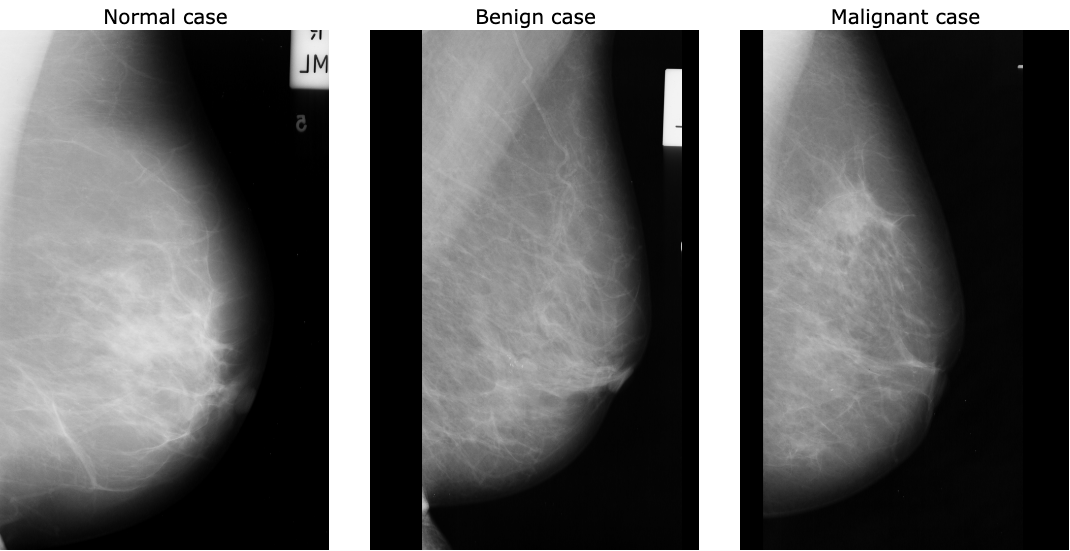
\includegraphics[width=\textwidth]{figures/introduction/mammogram examples.png}}
\caption{\label{fig:introduction-mammogram-examples}Example of three types of mammograms, including normal, benign and malignant cases. Figures extracted from the mini-MIAS dataset (Suckling, 1994). Created using draw.io.}
\end{figure}

Error-prone mammogram interpretations by radiologists can lead to decisions that can ultimately harm the patients. If a mammogram is diagnosed as malignant, breast biopsies (extraction of cells in breast tissue) are usually prescribed. However, 40-60\% of biopsies are diagnosed as benign, clearly betraying the necessity for correct mammography diagnosis to avoid needless operations, anxiety and pain for the patients \citep{Hepsag2017}. On the one hand, breast cancers can be missed altogether, inducing an absence of treatments for sick patients, while on the other hand, an instance of breast cancer can be reported when in reality there is no cancerous tumour, leading to unnecessary treatment being carried out \citep{Elter2009}.\\

To that end, using Computer-Assisted Detection (CAD) software can help minimise the number of wrong interpretations and increase the accuracy of mammography screening \citep{Shen2017}.\\

The motivation behind this project is to explore techniques for implementing a deep learning system that can accurately detect breast cancer in order to prevent late treatments due to false negatives as well as preventing unnecessary treatments in cases of false positives. Ultimately, the long-term target of this project is to combine it with other deep learning algorithms developed across other projects supervised by Dr David Harris-Birtill (past and present). This will allow a general artificial intelligence system capable of detecting multiple forms of cancer with higher accuracies than radiologist diagnoses.\\

%%%%%%%%%%%%%%%%%%%%%%%%%%%%%%%%%%%%%%%%%%%%%%%%%%%%%%%%%%%%%%%%%%%%%%%%%%%%%%%%%%

\section{Problem Description}
\label{sec:problem-description}

CAD systems using deep learning techniques could, in theory, highly increase the accuracy of mammogram screenings for detecting early signs of breast cancers. However, these techniques require large amounts of data to learn the cancer's underlying patterns and adapt to new cases, and require  powerful computing resources to accelerate the process of learning the data, making them very hard to optimise.\\

Parts of the work undertaken during this project will be conducted as a group comprised of two other members, Ashay Patel and Shuen-Jen Chen. Section~\ref{sec:introduction-objectives} covers which tasks will be conducted personally/in a group in more detail. The reasoning behind these common tasks is for a functional pipeline to be reached earlier, eventually allowing each group member to further explore deep learning techniques individually more quickly due to the limited time frame of this project, using the common primary pipeline as a baseline.

%%%%%%%%%%%%%%%%%%%%%%%%%%%%%%%%%%%%%%%%%%%%%%%%%%%%%%%%%%%%%%%%%%%%%%%%%%%%%%%%%%

\section{Objectives}
\label{sec:introduction-objectives}

The main objective of this project consists of implementing a deep learning pipeline that will be able to learn how to detect cases of breast cancer in mammograms. This objective is broken down into two steps:
\begin{itemize}
    \item \textbf{Group work}: a common deep learning pipeline will be initially implemented as part of a group with Ashay Patel and Shuen-Jen Chen over the course of a three-week period, including data cleaning and pre-processing, results output and a basic deep learning model. The distribution of tasks between the group can be found in Appendix~\ref{ch:appendix-team-meeting-summaries}.
    \item \textbf{Individual work}: the pipeline above will then be individually extended and evaluated by using various deep learning techniques.
\end{itemize}

An extensive context survey has to first be conducted to cover the background of deep learning techniques applied to the field of cancer detection and to review existing results. This includes identifying results achieved using different methods (e.g. traditional machine learning techniques). This step is primordial as it will guide the research towards the most promising areas, as well as govern the choice of techniques to implement and explore in further chapters.\\

Finally, the final results achieved individually will be compared with the baseline pipeline created as a group, as well as the results found in papers that used the same datasets.

%%%%%%%%%%%%%%%%%%%%%%%%%%%%%%%%%%%%%%%%%%%%%%%%%%%%%%%%%%%%%%%%%%%%%%%%%%%%%%%%%%

\section{Report Structure}

\tab \textbf{Introduction} \space 
Presents an overview of the subject's background through the problem description and the motivation behind this project, followed by the objectives that the project aims to achieve.\\

\textbf{Context Survey} \space
Explores the literature and background surrounding breast cancer detection techniques, starting from primitive cancer detection systems, followed by traditional machine learning methods, and ending with the deep learning techniques that have been recently used.\\

\textbf{Ethics \& Datasets} \space
Considers the ethical issues taken into account for this project and describes the datasets used.\\

\textbf{Design} \space
Explores high-level design considerations regarding the deep learning pipeline to implement and the software in general.\\

\textbf{Implementation} \space
Comprehensively covers the steps followed when implementing the deep learning pipeline, explaining the practical solutions followed.\\

\textbf{Evaluation} \space
Reviews the different results to assess the efficiency of the different techniques used to train the model and how it compares to other models, including the common pipeline, the baseline and relevant results identified in the context survey.\\

\textbf{Conclusions} \space
Summarises the project's accomplished objectives, its limitations, plans for future work, and a final reflection on the project as a whole.


\chapter{Context Survey}
\label{ch:chapter-litsurvey}
%%%%%%%%%%%%%%%%%%%%%%%%%%%%%%%%%%%%%%%%%%%%%%%%%%%%%%%%%%%%%%%%%%%%%%%%%%%%%%%%%%
% 1
%%%%%%%%%%%%%%%%%%%%%%%%%%%%%%%%%%%%%%%%%%%%%%%%%%%%%%%%%%%%%%%%%%%%%%%%%%%%%%%%%%

\section{Breast Cancer Detection}

\subsection{Medical imagery screening tests \& biopsies}
\label{sec:litreview-bcd-medical-imagery}

Test screenings have been used to detect early signs of breast cancer before the appearance of any symptoms, e.g. lumps that can be felt to the touch of a hand. The main methods used for breast cancer screenings are \textit{mammograms}, which are low-dosage x-rays around the breast area usually  used as initial/regular screening tests. This screening method is followed by \textit{breast ultrasounds} for analysing masses such as lumps or cysts, and by \textit{breasts MRI} (Magnetic Resonance Imaging) for detailed imagery of the breast, usually used when a malignant tumour has been detected to get more information about it, such as its size and location, or to find additional ones \citep{americanCancerSociety2019}. If any of the screenings mentioned earlier raise suspicion or reveal a potential presence of breast cancer, then biopsies can be conducted to confirm the screening tests' results. Biopsies consist of extracting cells or a small part of the breast's tissue that are sent to a lab to be analysed by pathologists to get definite results \citep{martin2019}.\\

Due to the invasive nature of biopsies, it is ideal for patients to use medical imagery tools to detect early signs of breast cancer that can be treated efficiently rather than immediately conducting a biopsy. Mammograms are the primary imagery method used for early breast cancer detection (BCD) \citep{Ramos-Pollan2012}. However, breast cancer detection using mammograms, and any form of cancer using medical imagery, relies on the conventional diagnoses of expert radiologists \citep{Osareh2010}. These diagnoses rest on the correct interpretation of the mammograms, which may be subject to errors due to the difficulty of correctly interpreting them \citep{Elter2009}. Indeed, mammograms are 2D images of 3D breasts that correspond to the superposition of breast tissue, which increases the difficulty for a radiologist to correctly analyse patterns as masses often naturally form due to this superposition \citep{Elter2009}.

\subsection{Early Breast Cancer Detection Systems}
\label{sec:litreview-bcd-early-cad}

To assist radiologists in their interpretations of mammograms, Computer-Assisted Detection/Diagnosis (CAD) software has been employed since the 1970s. However, pre-1990s CAD systems were very primitive and did not offer much more knowledge than the expert radiologists' knowledge. These unsophisticated ``expert'' systems consisted of manually processing and modelling pixels to construct rule-based systems that mainly used \textit{if-else-then} statements \citep{Litjens2017}, highlighting their inadequacy to learn how to recognise patterns that can be used to detect breast cancer.

\subsection{Towards Supervised Machine Learning-based Systems}

Towards the late 1990s, supervised machine learning techniques started replacing these expert systems, allowing hidden patterns in the mammograms' data that could not be perceived by radiologists to now be recognised by these new algorithms \citep{Litjens2017}. Machine learning-based approaches were selected over statistical approaches as they were more performant when dealing with large, complex and high-dimensional datasets \citep{Yue2018}, which is the case of datasets of mammograms. Additionally, machine learning methods were proven to be more suitable for the task of classification than traditional statistics-based approaches such as regression \citep{Paliwal2009}, marking the shift from CAD systems that were fully designed by humans to systems that were trained on datasets of medical imagery \citep{Litjens2017}.\\

However, these machine learning models could not accurately operate on purely raw data such as the full-sized mammogram images. Indeed, all of the machine learning models tested against the task of breast cancer detection required relevant pieces of information to first be extracted from the image to solve the given task, such as k-Nearest Neighbour [kNN], Decision Trees [DT], Naive Bayes [NB] \citep{Asri2016}, Support Vector Machines [SVM] \citep{Ramos-Pollan2012} and Artificial Neural Networks [ANN] \citep{Yue2018}. These crucial bits of information pulled from the mammograms data correspond to features, and need to be extracted by humans before being fed to the aforementioned models for training. These features range from visual information, such as colours, edges, corners, shapes and textures \citep{Geron2019}, to extracted information, such as the cell size, clump thickness, bare  nuclei, etc. \citep{Yue2018}.\\

Logically, the next step in the evolution of breast cancer detection systems is for the model to learn these features on its own directly from the data rather than being fed hand-extracted features \citep{Yala2019}. Deep learning models, which corresponds to neural networks with hundreds of hidden layers, are based on this concept and are covered in Section~\ref{sec:litsurvey-DLtechniques-CNN}. However, these models have not been successfully implemented until recent years as they require powerful computers, usually equipped with Graphical Processing Units (GPU) to be efficiently trained. This means that until recent years, the machine learning models discussed in Section~\ref{sec:litreview-MLmodel-BCDapplications} have led the field of breast cancer detection, with some manual mammogram interpretations still being carried out by radiologists \citep{Litjens2017}, as depicted in Figure~\ref{fig:litsurvey-bcd-timeline}.

\begin{figure}[ht]
\centerline{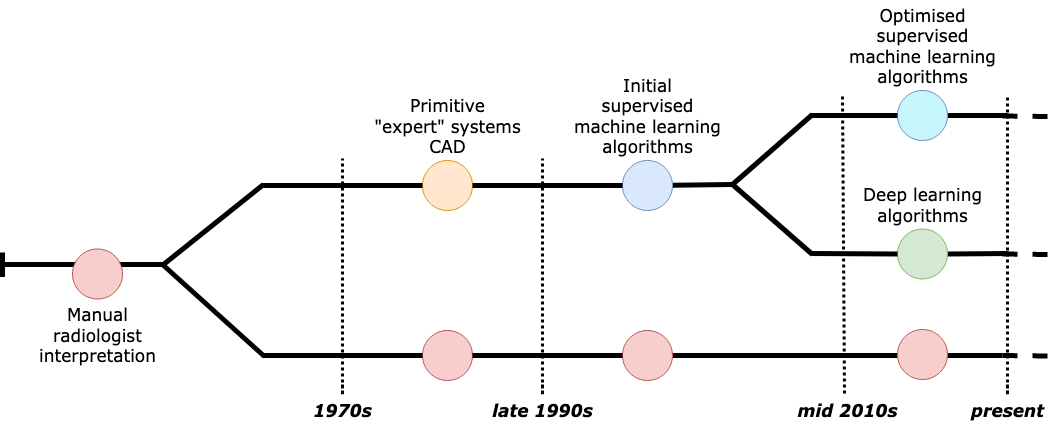
\includegraphics[width=\textwidth]{figures/litsurvey/bcd_timeline.png}}
\caption{\label{fig:litsurvey-bcd-timeline}Timeline of the evolution of breast cancer detection systems synthesising the information described in Sections~\ref{sec:litreview-bcd-medical-imagery}~and~\ref{sec:litreview-bcd-early-cad}.}
\end{figure}

%%%%%%%%%%%%%%%%%%%%%%%%%%%%%%%%%%%%%%%%%%%%%%%%%%%%%%%%%%%%%%%%%%%%%%%%%%%%%%%%%%
% 2
%%%%%%%%%%%%%%%%%%%%%%%%%%%%%%%%%%%%%%%%%%%%%%%%%%%%%%%%%%%%%%%%%%%%%%%%%%%%%%%%%%

\section{Machine Learning Tasks \& Algorithms}
\label{sec:litreview-MLmodel-BCDapplications}

\subsection{Machine Learning Applications to Breast Cancer Detection}

\subsubsection{Types of machine learning algorithms}

Machine learning algorithms fall in different categories based on whether human supervision is required or not. The two main types of machine learning algorithms correspond to supervised and unsupervised learning. On the one hand, in supervised learning, the dataset is labelled, meaning every sample in the dataset includes a solution \citep{Geron2019}. This label, often noted $y$, is used to make a prediction $\hat{y}$ by fitting the input features $\textbf{x}$ from a training dataset. The goal of a supervised learning algorithm is to determine the optimal parameters $\theta$ for the selected algorithm in order to minimise a loss function defined as $L(y,\hat{y})$, which corresponds to the error between the predicted algorithm's output $\hat{y}$ and the real output $y$ \citep{Litjens2017}. A large variety of loss functions can be used such as the general Mean Squared Error (MSE) and Mean Absolute Error (MAE) loss functions, or more specific loss functions such as the Hinge Loss for SVMs \citep{Geron2019}. The main applications of supervised learning are classification and regression, with the former being the most relevant to breast cancer detection.\\

On the other hand, in unsupervised learning, the data is unlabelled, meaning only the input features $\textbf{x}$ are available while the labels $y$ are not \citep{Litjens2017}. This means the algorithm cannot optimise its hyperparameters, which correspond its configurations used to define it before training \citep{Bergstra2013}, by minimising a loss function. Instead, the algorithm needs to automatically create clusters in the dataset in order to separate them into different groups. The main applications of unsupervised learning are clustering, anomaly detection, data visualisation and dimensionality reduction \citep{Geron2019}, rendering them irrelevant to breast cancer detection. Two other categories of machine learning algorithms exist, corresponding to semi-supervised learning and reinforcement learning, but are also irrelevant to the task of detecting breast cancer.\\

Among the two types of machine learning algorithms, the most pertinent one for the task of breast cancer detection is supervised learning as datasets of mammograms need to contain properly labelled data for each sample, indicating the status of the mammogram, i.e. no tumour, benign tumour, malignant tumour \citep{Shen2017}.

\subsubsection{Types of machine learning tasks}

Two types of machine learning tasks are very relevant to medical imagery analysis, including mammogram analysis for breast cancer detection: \textit{detection} (classification) and \textit{segmentation} \citep{Litjens2017}. 

\paragraph{Detection} corresponds to the classification of a medical image or exam, which is an interpretation that used to be entirely carried out by a radiologist before the appearance of CAD systems (see Section~\ref{sec:litreview-bcd-early-cad}). The classification can be either binary or multi-class depending on the data used. With datasets like the ``Curated Breast Imaging Subset of DDSM'' \citep{Lee2017}, the classification is binary as mammograms can only be classified as either ``benign'' or ``malignant''. However, when using datasets like the ``Digital Database for Screening Mammography'' \citep{DDSMdataset2001}, the classification becomes more interesting from a clinical point of  view as mammograms can either be classified as ``normal'', ``benign'' or ``malignant'' \citep{Litjens2017}. An example of classification between benign and malignant mammograms can be found in Figure~\ref{fig:classification_example}, reinforcing the complexity that comes with interpreting mammograms for radiologists and the need for accurate and reliable CAD systems to improve the prediction accuracies.

\begin{figure}[h]
\centering
\begin{subfigure}{.5\textwidth}
  \centering
  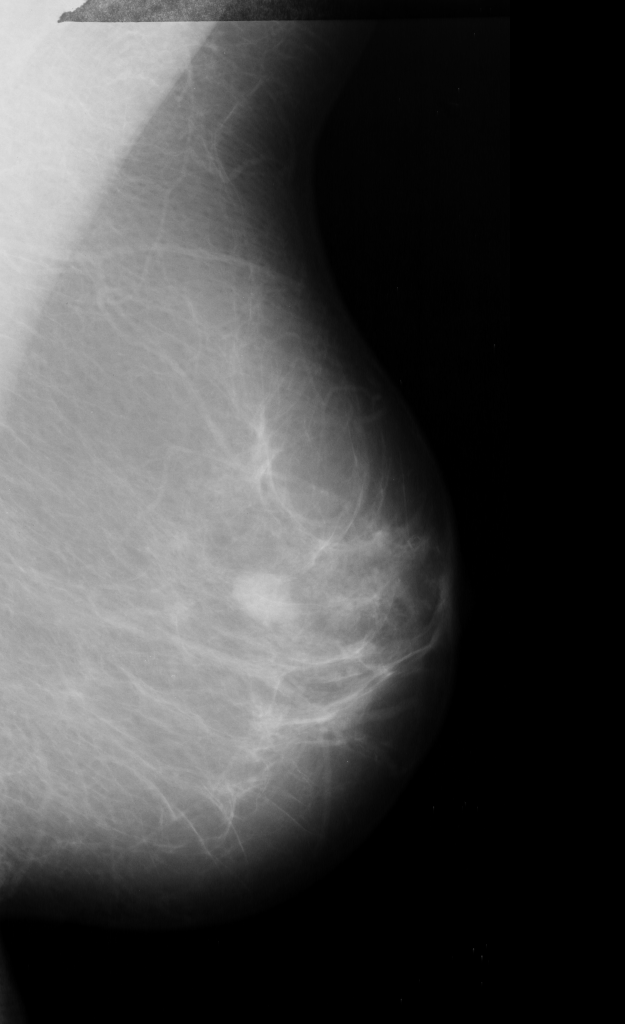
\includegraphics[width=0.5\textwidth]{figures/litsurvey/classification_benign.png}
  \caption{A benign mammogram.}
  \label{fig:classification_benign}
\end{subfigure}%
\begin{subfigure}{.5\textwidth}
  \centering
  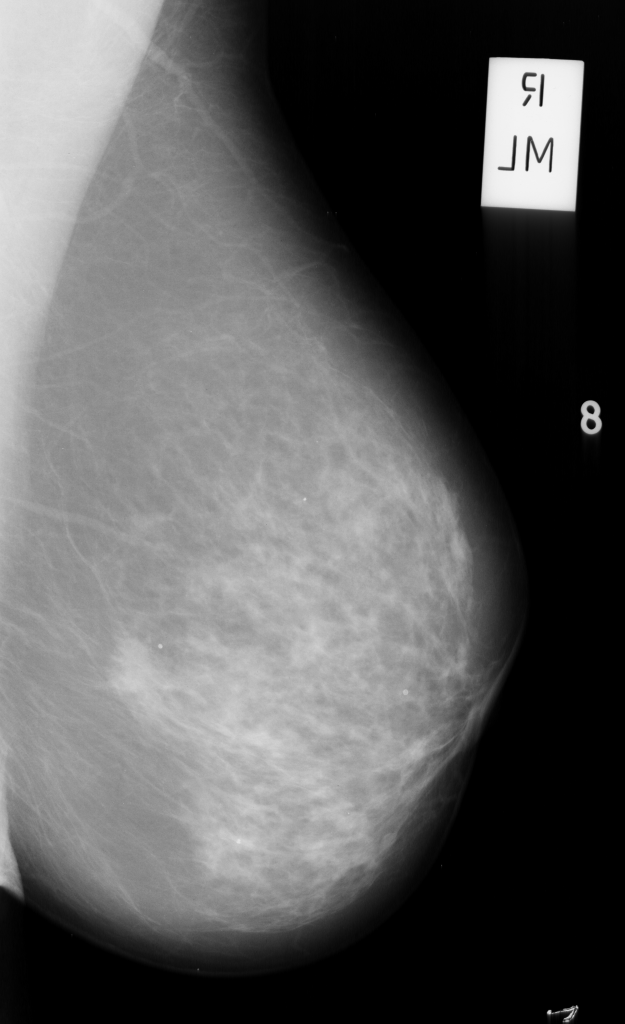
\includegraphics[width=0.5\textwidth]{figures/litsurvey/classification_malignant.png}
  \caption{A malignant mammogram.}
  \label{fig:classification_malignant}
\end{subfigure}
\caption{\label{fig:classification_example}Example of a breast mammogram classification, showing benign (left) and malignant (right) mammograms. Images retrieved from the mini-MIAS dataset (Suckling, 1994).}
\end{figure}

\paragraph{Segmentation} corresponds to the classification of each pixel in the image based on the class of the object the pixels belongs to, without distinguishing objects from the same class. All objects belonging to the same class will be classified in the same grouping of pixels \citep{Geron2019}. In breast cancer detection, segmentation can be used to highlight masses such as calcifications, cysts or fibroadenomas \citep{breastcancerorg2018} in mammograms by separating the masses from the background. An example is shown in Figure~\ref{fig:segmentation_example}, where mammograms are partitioned into non-overlapping segments, revealing potential masses in the image \citep{Punitha2018}.\\

\begin{figure}[h]
\centering
\begin{subfigure}{.5\textwidth}
  \centering
  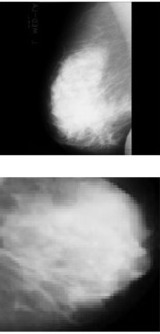
\includegraphics[width=0.52\textwidth]{figures/litsurvey/segmentation_example_original.jpg}
  \caption{Original mammogram images.}
  \label{fig:original-mammogram}
\end{subfigure}%
\begin{subfigure}{.5\textwidth}
  \centering
  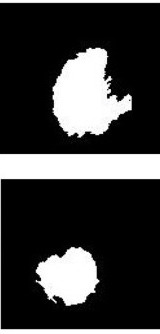
\includegraphics[width=0.52\textwidth]{figures/litsurvey/segmentation_example_segmented.jpg}
  \caption{Segmented mammogram images.}
  \label{fig:segmented-mammogram}
\end{subfigure}
\caption{\label{fig:segmentation_example}Example of a breast mammogram segmentation, showing the original mammogram (left) and the segmented image (right), depicting large masses. Images retrieved from Punithaet al. (2018).}
\end{figure}

Other machine learning tasks that have been used in medical imagery analysis consist of content-based image retrieval (retrieving similar images from a database) or image enhancement (erasing obstructing elements from an image and increasing quality) \citep{Litjens2017}, but will not be further explored as they are not directly relevant to the task of breast cancer detection. Indeed, the task of classification (detection) can be used to interpret whether a breast is affected by cancer through the analysis of databases of mammograms, while the task of segmentation can be used to localise a tumour within a breast by finding regions that may correspond to masses, pinpointing potential danger areas that may lead to cancerous cells.

\subsection{Comparison of BCD Supervised Learning Algorithms}

Since the late 1990s, a rich array of supervised machine learning algorithms have been applied and tested against the task of breast cancer detection, yielding varying results, but ultimately contributing to improving accuracies for detecting breast cancer \citep{Yue2018}. The main types of algorithms used in breast cancer detection, which consist of k-Nearest Neighbour (kNN), Naive Bayes (NB), Support Vector Machines (SVM), Decision Trees (DT) and Artificial Neural Networks (ANN), are briefly explained in the ensuing sections from most simple to most complex. Their performances, when applied to the task of breast cancer detection, are then compared to draw a picture of the advantages and disadvantages that each method brings.

\subsubsection{k-Nearest Neighbours}
\label{sec:litreview-knn}

k-Nearest Neighbours (kNN) is one of the simplest machine learning algorithms and is often used as an initial benchmark when studying a dataset with no prior knowledge \citep{peterson2009k}. It is a non-parametric and lazy model, as it does not learn the data's pattern but rather classifies a test sample by looking at its $k$ nearest neighbours \citep{Yue2018}. The sample data point's nearest neighbours are determined by using distance metrics such as the Euclidian distance, defined by Equation~\ref{eq:euclidian-distance} ($n$-dimensional space between two data points $s$ and $p$) which is the most widely used metric \citep{peterson2009k}. Figure~\ref{fig:litsurvey-knn-example} depicts an example of how a kNN classifier would be used to distinguish between a benign and a malignant tumour using $k=3$.

\begin{equation}
\label{eq:euclidian-distance}
    d(s,p)=\sqrt{\sum_{i=1}^{n}(s_i-p_i)^2}
\end{equation}

\begin{figure}[h]
\centerline{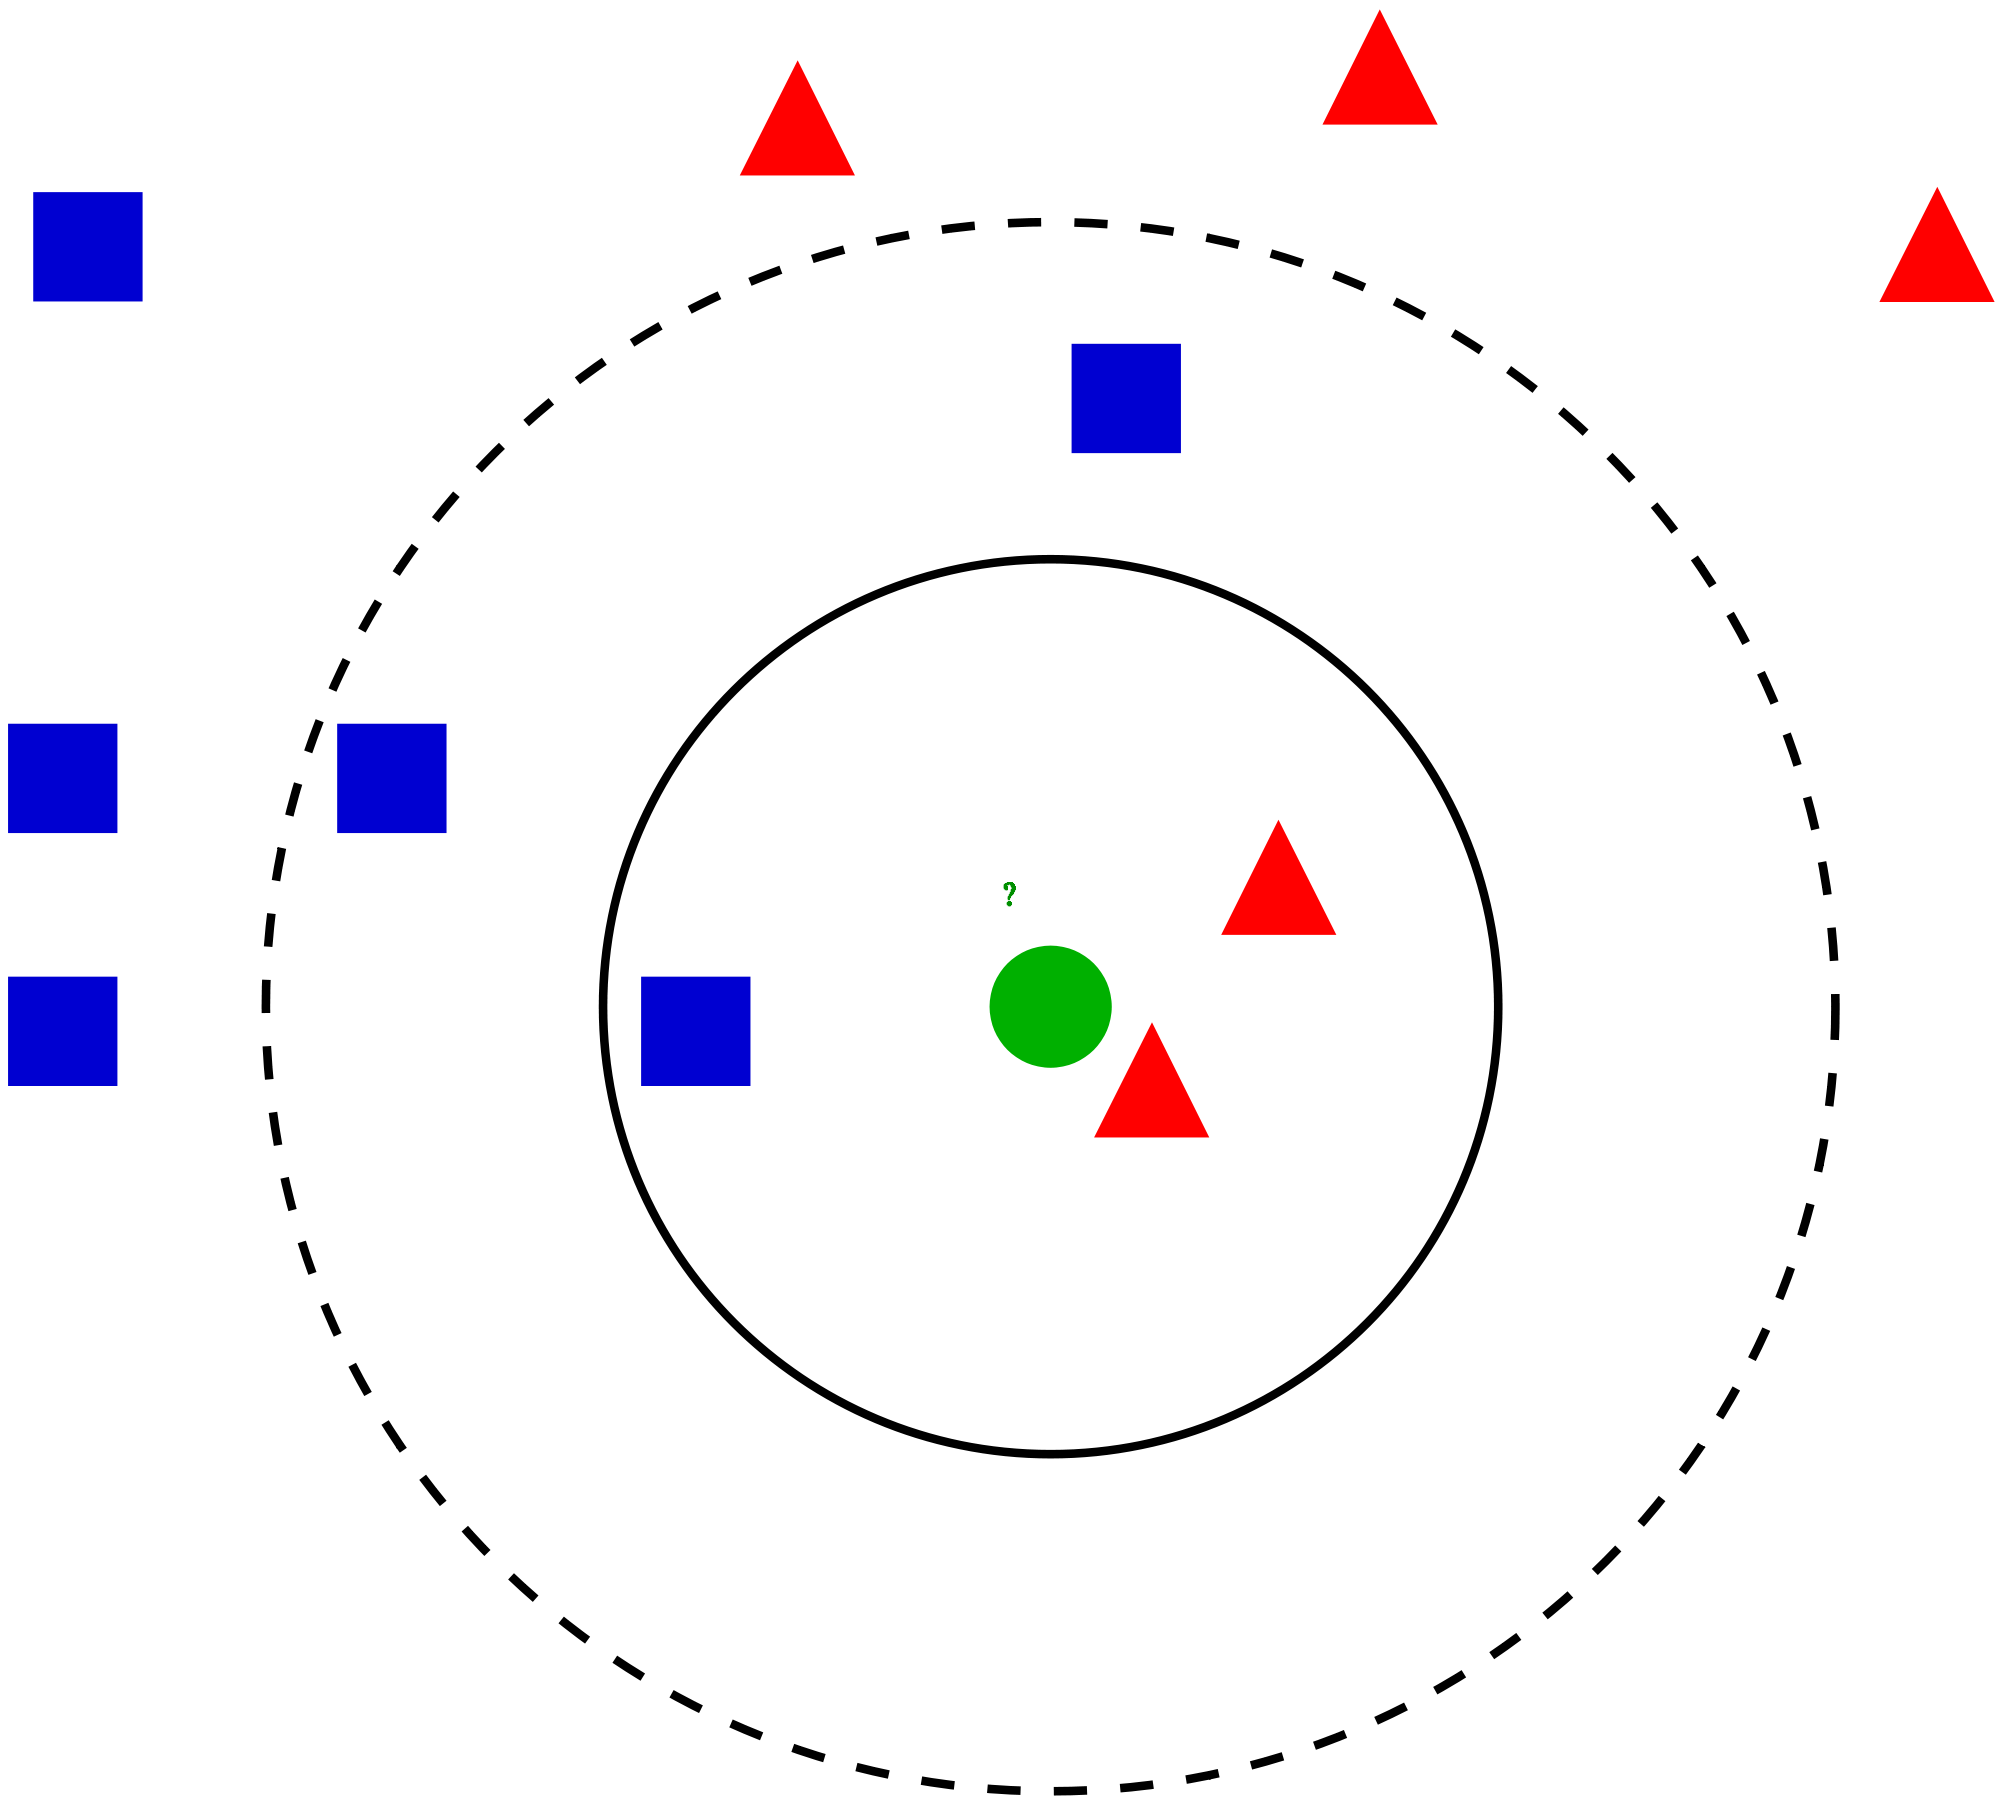
\includegraphics[width=0.4\textwidth]{figures/litsurvey/knn.png}}
\caption{\label{fig:litsurvey-knn-example}Example of a kNN classifier distinguishing between benign (blue square) and malignant (red triangle) tumours for a test data sample (green circle) using $k=3$. The test sample is classified as malignant as there are two red triangles and one blue square amongst the three neighbours. Figure retrieved online from T. Srivastava (\url{https://tinyurl.com/y3jqco49}).}
\end{figure}

Generally used as an initial learning algorithm to experiment with new datasets, the kNN algorithm has been tested on distinctive datasets of mammograms for breast cancer detection such the ``Wisconsin Breast Cancer Wisconsin'' (WBCD) dataset, which contains ten extracted features such as clump thickness, cell size/shape, etc. \citep{Wolberg1995}. kNNs calibrated with $k=1$ and using the Euclidian distance achieved 98.25\% accuracy \citep{Sarkar2000} and 98.70\% accuracy \citep{AhmedMedjahed2013} on the WBCD dataset when compared with other values of $k$ ranging from 1 to 15 and using other distance metrics such Cityblock distance, cosine distance and correlation.\\

Despite Sarkar et al. and Medjahed et al. reporting that a value of $k=1$ seemed to yield the most accuracy, these 1-NN classifiers do not actually learn the data's patterns and often underperform compared to other classifiers mentioned below, especially compared to SVMs and ANNs which can surpass accuracies of 99\% \citep{Yue2018, Asri2016, Montazeri2016}. Nevertheless, the results achieved by kNN remain fruitful when used as a primary benchmark before testing more advanced models, such as the ones described below.

\subsubsection{Naive Bayes}

Naive Bayes uses Bayes' theorem and the assumption that all input features are independent from one another, which can be described as the input features $\textbf{x}=(\textbf{x}_1, ..., \textbf{x}_n)$ being independent given a class label $C$ in Equation~\ref{eq:naive-bayes} \citep{rish2001empirical}.

\begin{equation}
\label{eq:naive-bayes}
    P(\textbf{x}|C)=\prod_{i=1}^{n}P(\textbf{x}_i|C)
\end{equation}

This assumption leads to a naive model that despite not learning the data's underlying pattern (in a similar fashion to kNN), still offers competitive results in practice \citep{russell2002artificial}, notably in the field of medical imagery analysis \citep{rish2001empirical}. Naive Bayes achieves an accuracy of 93\% on the WBCD dataset \citep{Kharya2014}, which is comparable to the aforementioned 1-NN classifiers as it does not learn the data's patterns and use extracted features rather than the original mammograms. NB still remains useful for assessing benchmark classification to compare with more advanced models.

\subsubsection{Decision Trees}
\label{sec:litsurvey-dts}

Unlike kNN and NB, the decision tree algorithm is a simple yet powerful one that fits the data. It works like a flowchart mapping samples' input feature vectors attributes and values, creating a tree made up of different types of nodes. Each non-leaf nodes tests one of the feature vectors attributes, branching out to a deeper node based on the attribute's value. Once a leaf node is reached after multiple tests, a classification decision is made \citep{quinlan2014c4}. An example of a decision tree applied to breast cancer detection can be found in Figure~\ref{fig:litsurvey-dt-example}, illustrating how attributes and their values are used to classify a tumour as benign or malignant.\\

\begin{figure}[ht]
\centerline{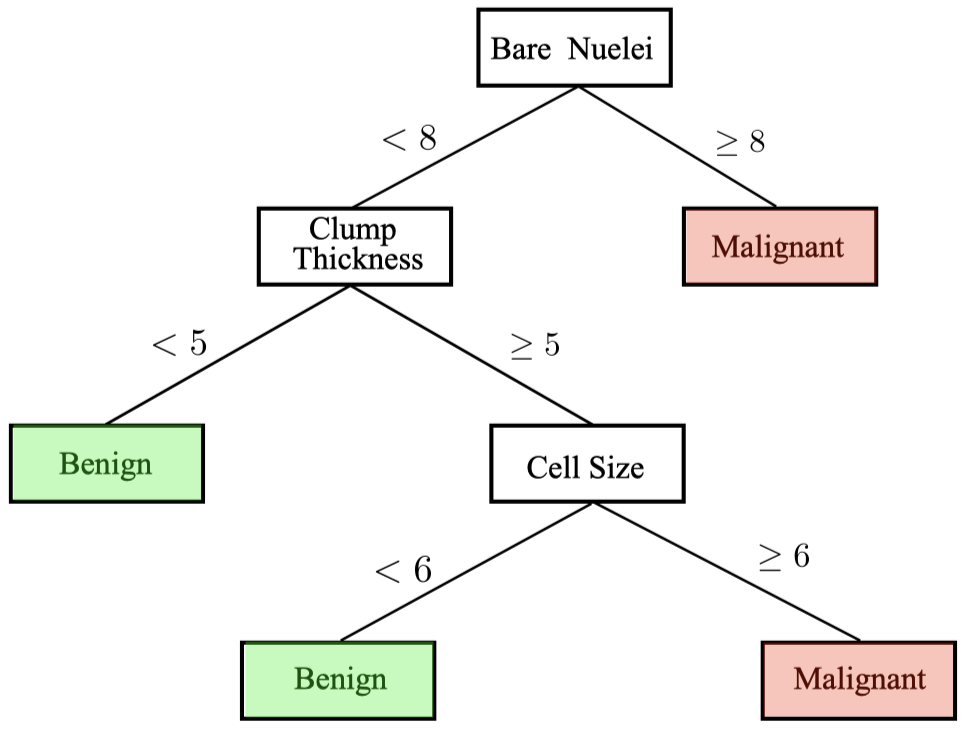
\includegraphics[width=0.65\textwidth]{figures/litsurvey/dt.png}}
\caption{\label{fig:litsurvey-dt-example}Example of a decision tree classifier distinguishing between benign and malignant tumours based on three extracted features from a dataset of mammograms: the size of the bare nuclei, the thickness of the clump and the uniformity of the cell size. Figure created by Yue et al. (2018).}
\end{figure}

The most popular implementations of decision trees use entropy-based impurity metrics to generate the tree, such as the ID3, C4.5 and C5.0 decision tree algorithms \citep{Yue2018}. A node reaches an entropy value of 0 when it is ``pure'', i.e. it contains only instances of one class (either only benign or only malignant data samples) \citep{Geron2019}.\\

The extra complexity offered by decision trees such as the C4.5 classifier does do not offer improved results compared to kNN and NB classifiers, with 94.56\% achieved using J48 (Java implementation of C4.5) on the WBCD dataset \citep{Sumbaly2014}, which is still falling short of the performance achieved by SVMs and ANNs, which can exceed the 99\% threshold \citep{Yue2018}. Nevertheless, inserting decision trees into hybrid systems by combining them with other machine learning algorithms such as SVMs and NBs increases the accuracy to 97.13\% on the WBCD dataset \citep{Kumar2017}, which are closer to those achieved by SVMs and ANNs \citep{Yue2018}. Indeed, these hybrid systems use the advantages of each method, cancelling out the negatives of each, but come at the cost of being complicated to engineer and still requiring handcrafted features to be fed to them as input, which is confirmed by their decision of testing these algorithms on the WBCD dataset rather than datasets containing raw images like DDSM.

\subsubsection{Support Vector Machines}
\label{sec:litsurvey-svms}

An SVM consist of a \textit{maximal margin classifier}, which aims to find the hyperplane that separates two classes the most, and the \textit{kernel trick}, used to separate non-linear data. In Figure~\ref{fig:litsurvey-svm-example}, a visual example of a maximum margin hyperplane to separate linearly separable benign and malignant tumours is shown.\\

\begin{figure}[ht]
\centerline{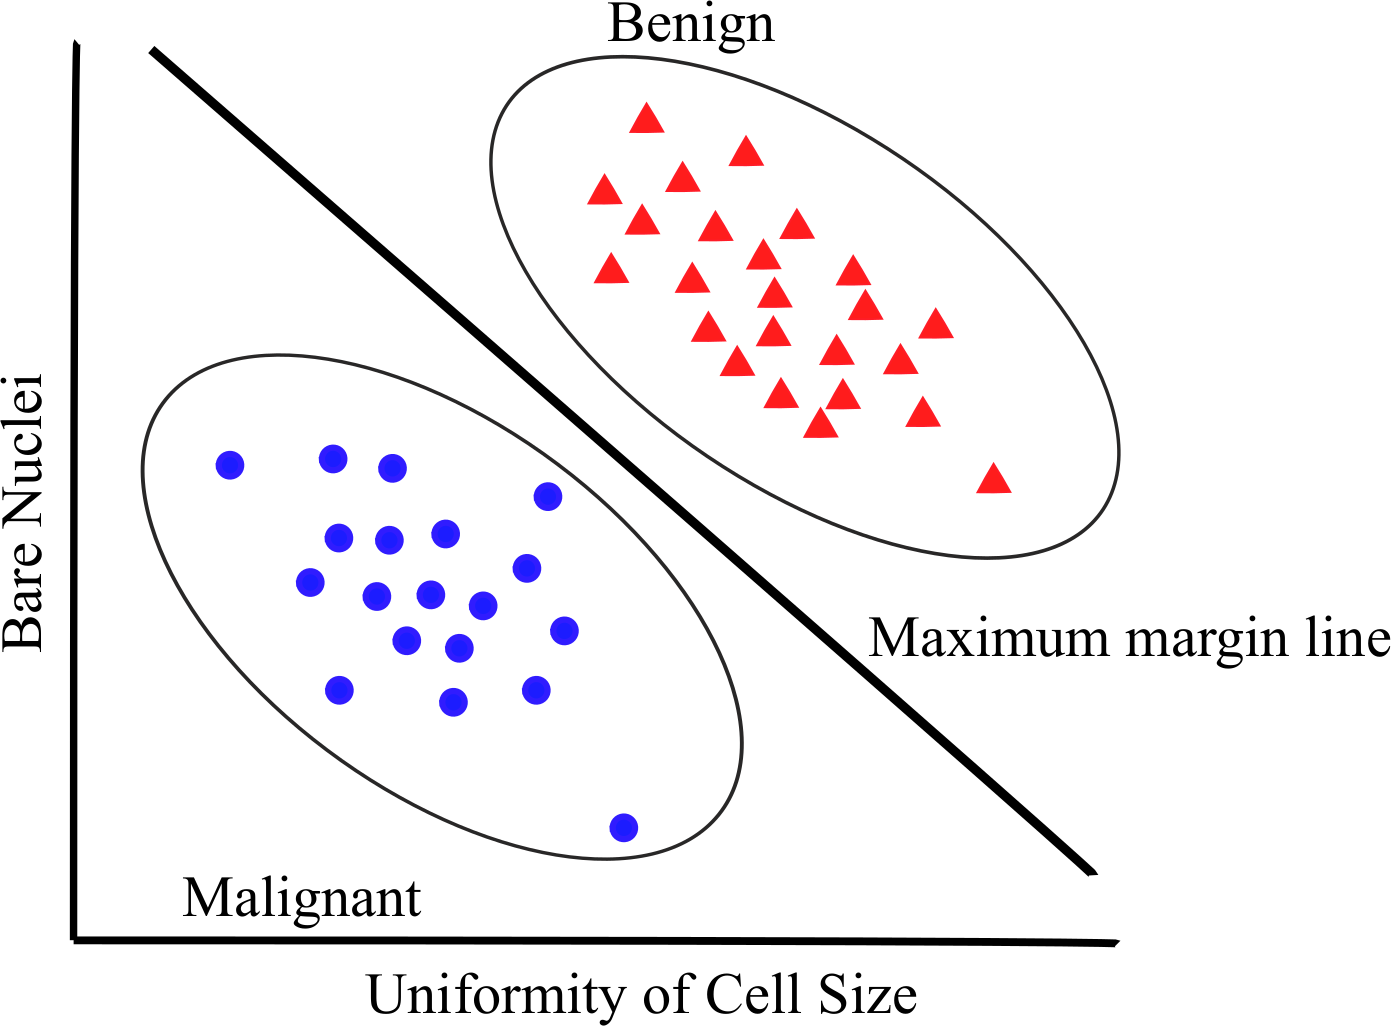
\includegraphics[width=0.6\textwidth]{figures/litsurvey/svm.png}}
\caption{\label{fig:litsurvey-svm-example}Example of a SVM classifier's maximum margin hyperplane found to separate benign and malignant tumours based on two extracted features from a dataset of mammograms: the size of the bare nuclei and the uniformity of the cell size. Figure created by Yue et al. (2018).}
\end{figure}

In the case of non-linear data, the training data is mapped to a higher dimension where they can be linearly separated. This is achieved by using the kernel trick, which maps the input feature vector to a higher dimension by using the dot product, but does not carry out the transformation, which would exponentially increase the size of the feature space and consequently the training time \citep{Geron2019}. This kernel trick is what allowed SVMs to become one of the most widely used machine learning models in many fields, including medical imagery analysis, up until today \citep{Yue2018}.

Many kernels can be chosen for SVM classification ranging from Polynomial kernel for image processing to Radial Basis Function (RBF) or Gaussian kernels for general tasks when there is no prior knowledge of the data), heavily influencing its performance \citep{amari1999improving}. For the task of breast cancer detection, RBF outperformed Polynomial kernels on two small datasets\footnote{``Fine needle aspirate of breast lesions'' (FNAB) dataset and ``gene microarrays'' dataset \citep{Osareh2010}.} containing extracted features, with the RBF kernel managing 98.80\% and 96.33\% accuracies on both datasets while Polynomial reached 97.09\% and 95\% accuracies \citep{Osareh2010}, depicting why RBF is often chosen over other kernels.\\

Compared to the previously mentioned ML methods, SVMs seem to learn the extracted features more efficiently, reaching 97.13\% accuracy on the WBCD, while kNN attained 95.27\%, NB 95.99\% and DT 95.13\% \citep{Asri2016}. When applied to datasets containing raw images such as CBIS-DDSM, SVMs coupled with feature extraction techniques such as grey-level co-occurrence matrices (GLCM) achieved 63.03\% accuracy \citep{Sarosa2018}; while on smaller datasets like  mini-MIAS, SVMs coupled with texture-based features extracted from pre-processed images resulted in 92\% accuracy \citep{Vishrutha2014}. An accuracy of 97.2\% was achieved using the simplest form of SVMs on the WBCD dataset \citep{Bennett1998}, while 99.51\% accuracy was reached with SVMs on the same dataset when selecting the five best features \citep{Akay2009}, clearly characterising the importance of feature selection and image processing techniques for ML algorithms such as SVMs.

\subsubsection{Artificial Neural Networks}
\label{sec:litsurvey-anns}

ANNs form the basis of contemporary deep learning and are at the heart of the techniques mentioned in Section~\ref{sec:litsurvey-DLtechniques-CNN}. Originally inspired by the neuron connections found in the human brain \citep{mcculloch1943logical}, ANNs correspond to a collection of neurons (units) that ``fire'' an output if the linear sum of its weighted inputs tops a threshold. These neurons are placed in hierarchical layers (input, hidden and output layers) which are connected via weighted links, leading to \textit{fully connected} neural network when all the neurons from one layer communicate with all the neurons in the following layer. Input layer neurons accept the feature vectors $\textbf{x}$, hidden layer neurons process the data and output layer neurons represent an outcome for the classification \citep{russell2002artificial}. Figure~\ref{fig:litsurvey-ann-example} depicts an example fully-connected ANN used to classify benign and malignant tumours using six input neurons, eight hidden neurons and one output neuron.\\

\begin{figure}[ht]
\centerline{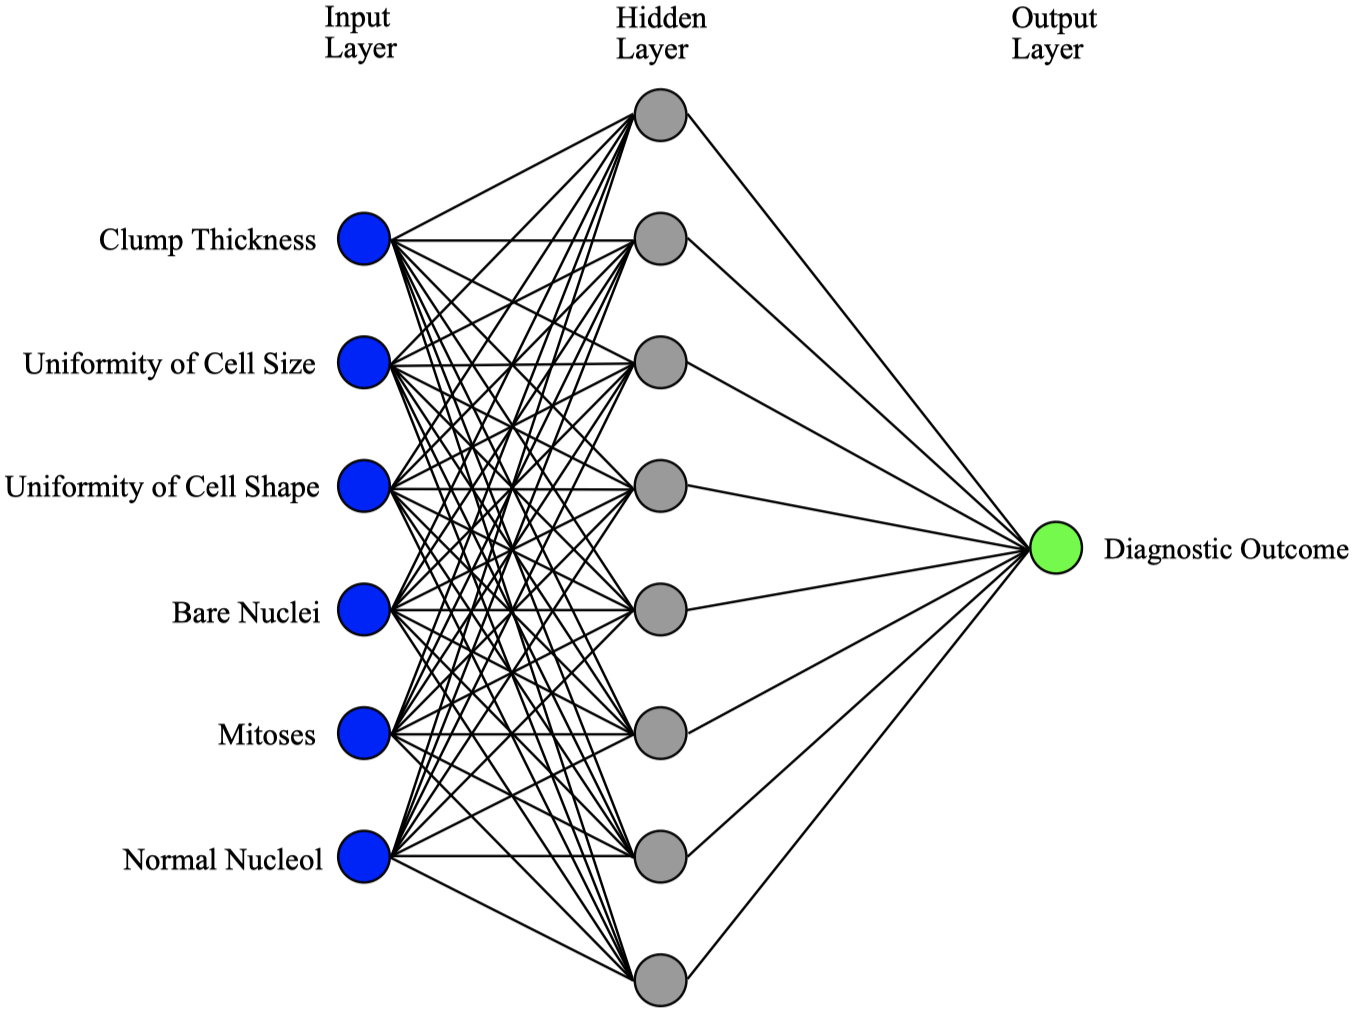
\includegraphics[width=\textwidth]{figures/litsurvey/ann.png}}
\caption{\label{fig:litsurvey-ann-example}Example of an ANN classifier distinguishing between benign and malignant tumours based on eight extracted features from a dataset of mammograms. Figure created by Yue et al. (2018).}
\end{figure}

Like the previous algorithms, neural networks learn by minimising the loss $L$ between the prediction $\hat{y}$ and the labels $y$. This is done via the backpropagation algorithm (BP), which propagates the error from the output layer back to the hidden layers, allowing the links' weights to be adjusted accordingly to minimise that error \citep{russell2002artificial}. The most common way to do this is by using MLE with Stochastic Gradient Descent (SGD) \citep{Litjens2017}. This learning ability found in ANNs is what gives them their potential, but also their complexity due to the large number of hyperparameters used to fine-tune them and their capacity to overfit the data when over-engineered. Indeed, combinations of neural networks hyperparameters may involve the network's structure (number of layers and neurons in each layer), the learning rate and momentum for SGD, the regularisation techniques and parameters, the activation functions and the stopping conditions to name a few \citep{sklearn-MLP-2019}.\\
 
Shallow ANNs, also referred to as Multi-Layer Perceptrons (MLP), immediately showed promising results when first applied to breast cancer detection, reaching 95.2\% accuracy with only a basic 3-layer architecture using BP \citep{Wu1993}, which already surpassed experts' predictions by 3\% to 5\% accuracy \citep{Yue2018}. However, due to computational constraints, deeper ANNs containing more hidden layers could not be efficiently utilised until recent years \citep{Litjens2017}. Instead, innovative variants to basic ANNs have been used to reduce training times, deal with multi-class classification with more ease, and yield predictions  with higher accuracies. Some of these ANN variants include networks such as Probabilistic Neural Networks (PNN) that replace the standard sigmoid activation function with an exponential function to find the training sample that is closest to the testing sample, achieving 97.23\% and 93.39\% accuracies on the two small datasets of extracted features (mentioned in Section~\ref{sec:litsurvey-svms}, which are larger than those achieved by kNN and Polynomial SVMs \citep{Osareh2010}. Another approach consisted of combining ANNs in hybrid systems (similar to those mentioned in Section~\ref{sec:litsurvey-dts}). When combined to Association Rule learning (AR) for reducing the number of features in the WBCD dataset from 9 to 5, ANNs and AR reached 95.6\% accuracy, which is extremely similar to the basic ANN on its own, but in almost half the epochs, converging in 33 epochs rather than 61 epochs, thus considerably reducing training time \citep{Karabatak2009}. Following that mindset of reducing the complexity of the WBCD dataset's features, Genetically Optimised ANNs (GOANN) use genetic programming (an ML technique that evolves towards a solution based on Darwin's theory of evolution) to determine the best features to use from the WBCD dataset and to optimise the network's weights and structure, producing an impressive accuracy of 99.26\% \citep{Bhardwaj2015}.

\subsubsection{Supervised machine learning algorithms comparison}

The five previously explored supervised machine learning algorithms all have one commonality: they heavily rely on the quality of the features extracted from the mammogram images as input to gain performance, and they cannot make use of the raw mammogram image in 2D space as input. This is confirmed by the datasets used for the task of BCD, as only datasets containing extracted features such as WBCD were used.\\

On their own, each algorithm showed limitations that prevent it from performing well. However, combined to form hybrid systems (e.g. DT + SVM + NB or ANN + AR), their performance increased in the form of higher accuracies or shorter training times, but so did their complexity to tune. It is worth noting that the slight differences when using identical algorithms on the same datasets can be due to the diverse training strategies involving unique training/testing/validation splits, image pre-processing steps and number of folds in cross-validation \citep{Yue2018}.\\

The next step for these supervised learning algorithms is to move away from feature extraction and redirect the effort towards new models that can automatically extract features from images rather than optimising and fine-tuning the hyperparameters and training strategies of existing algorithms. The most efficient way nowadays to achieve this is through Convolutional Neural Networks (CNN), which ingest the raw mammogram images in 2D space rather than extracted features or flattened images (transformed from 2D to 1D) where all spatial information is lost.

%%%%%%%%%%%%%%%%%%%%%%%%%%%%%%%%%%%%%%%%%%%%%%%%%%%%%%%%%%%%%%%%%%%%%%%%%%%%%%%%%%
% 3
%%%%%%%%%%%%%%%%%%%%%%%%%%%%%%%%%%%%%%%%%%%%%%%%%%%%%%%%%%%%%%%%%%%%%%%%%%%%%%%%%%

\section{CNNs \& Deep Learning techniques}
\label{sec:litsurvey-DLtechniques-CNN}

\subsection{Convolution Neural Networks}

\subsubsection{Motivation for CNNs over traditional neural networks}

CNNs are a type of neural network inspired by the human visual cortex, where neurons have local receptive fields that only react to visual stimuli originating from a region of the visual field. The combination of all receptive fields covered by overlapping neurons forms the whole visual field \citep{Geron2019}. This architecture makes them very efficient at performing complex visual tasks, marked by the first milestone for CNNs with the LeNet-5 architecture trained to recognise handwritten bank cheque digits \citep{LeCun1998}.\\

CNNs differ from traditional ``shallow'' ANNs as they are not fully connected. Indeed, CNNs are partially connected, with neurons in one layer only connected to a few neurons from the previous layer, meaning that they can work with large images \citep{Geron2019}. In a fully-connected neural network with only 100 neurons in the first layer, a 1,000 x 1,000-pixel image would already have 100,000,000 connections\footnote{$1000 \cdot 1,000 = 1,000,000$ px; $1,000,000$px $\cdot 100$ neurons $= 100,000,000$ connections.} in that first layer alone. CNNs nowadays can work with images thousands of pixel large, including the ones found in mammogram datasets described in Chapter~\ref{ch:chapter-ethics-datasets}, processing them much faster than traditional machine learning methods.

\subsubsection{CNN Structure}

The structure of CNNs builds on top of the concepts of traditional ANNs (see Section~\ref{sec:litsurvey-anns}) by piling stacks of convolutional layers and pooling layers that are followed by a fully connected network for classification (see Figure~\ref{fig:litsurvey-CNN-example}). The goal of the convolutional and pooling layers is to reduce the input images into a form that simple enough to be processed by other algorithms (the fully connected layers), retaining only useful information from the original image \citep{Shen2017}.

\begin{figure}[ht]
\centerline{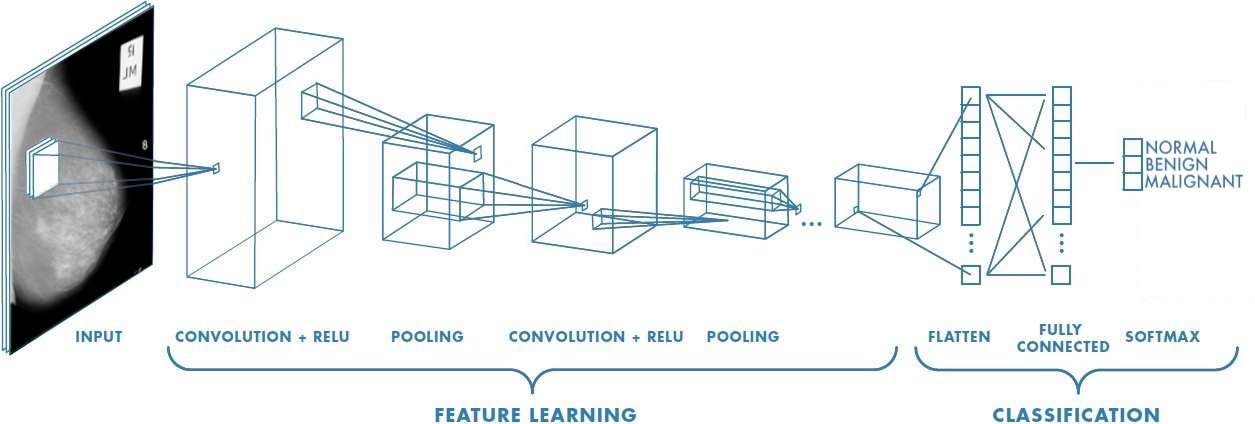
\includegraphics[width=\textwidth]{figures/litsurvey/CNN example.png}}
\caption{\label{fig:litsurvey-CNN-example}Example of a typical CNN adapted for multi-class breast cancer detection. Figure adapted from S. Saha (\url{https://tinyurl.com/y9mmosuq}).}
\end{figure}

\paragraph{Convolution Layers}

Neurons in the first convolutional layers are only connected to pixels in their receptive fields and not connected to every pixel in the image. Similarly, neurons in deeper convolutional layers are only connected to neurons in a small zone from the previous layer. This allows CNNs to first focus on low-level features, which are progressively assembled into high-level features as they get deeper. The more the receptive fields are spaced out (referred to as the stride), the smaller the next layer will be, thus considerably reducing the complexity of the CNN \citep{Geron2019}. Convolution is the mathematical operation that slides a moving a filter $f$ over an image $I$ to calculate a weighted sum (see Equation~\ref{eq:2d-convolution}). This 2D operation is possible in CNNs as layers are represented in 2D space and do not need to be flattened into a 1D array like with traditional neural networks, thus preserving the spatial information of images \citep{szeliski2010computer}.

\begin{equation}
\label{eq:2d-convolution}
    \hat{I}(x,y)=(I*f)(x,y)=\sum_{k}\sum_{l}I(k,l)\cdot f(x-k, y-l)
\end{equation}

The weights of the neurons in convolutional layers correspond to the filters, which are learned during the training phase by using optimisation techniques such as gradient descent. These filters allow a layer of neurons to highlight the areas of the image that activate the filter the most. As each layer has multiple filters, different features can be simultaneously detected in the layer's input. The result of each filter on a convolutional layer's input (the output of the previous layer) corresponds to a feature map. These multiple features maps are all stacked together to form the convolutional layer's output.

\paragraph{Pooling Layers}

Pooling layers are similar to convolutional layers as neurons are only connected to neurons from a small region in the previous layer. The difference is that this layer is not trainable as its neurons have no weights. Indeed, it is only used to downsample the image as it traverses the network to diminish the load on the GPU. It does so by calculating an aggregate of its inputs based on a function, which can either be a maximum or an average function (see Figure~\ref{fig:litsurvey-max-vs-avg-pooling}). \textit{Maximum pooling} returns the maximum value of the covered portion of the image, whereas \textit{average pooling} returns the average of all values. Maximum pooling is the preferred option in CNNs as it retains the most robust features only and acts as a noise suppressant by discarding noisy activations \citep{Geron2019}.\\

\begin{figure}[ht]
\centerline{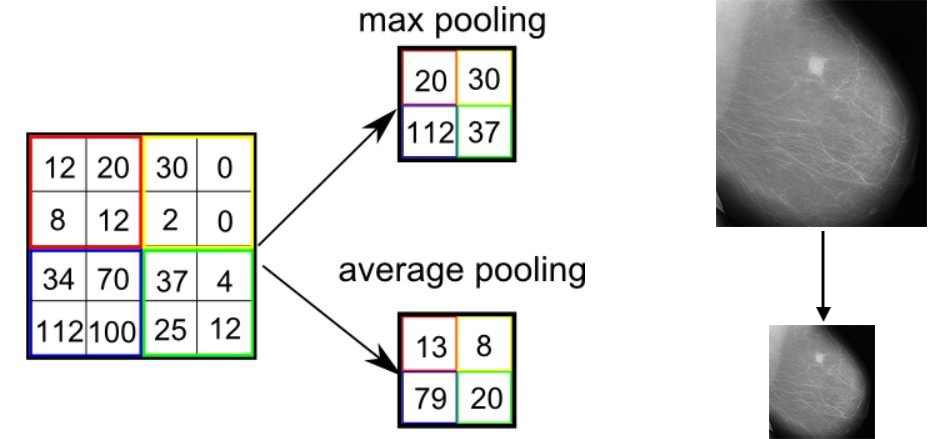
\includegraphics[width=\textwidth]{figures/litsurvey/max-vs-avg-pooling.png}}
\caption{\label{fig:litsurvey-max-vs-avg-pooling}Difference between max pooling and average pooling using a 2x2 window and stride 2 (left) to downsample an image (right). Figure adapted from W. Ong (\url{https://tinyurl.com/y25cke6l}).}
\end{figure}

Other benefits of pooling layers are the lower memory usage and the number of trainable parameters linked to smaller images, and especially the invariance it provides to the CNN as it will not break down when fed images that contain features of different sizes than the ones seen in the training dataset \citep{Shen2017}.

\paragraph{Fully connected layers \& Activation functions}

Similarly to ANNs, activation functions are used to connect the convolutional and spooling layers. The most common activation function used in CNNs is the Rectified Linear Unit (ReLU).\\

At the end of the stack of convolutional and spooling layers, a fully connected MLP is placed. This dense neural network takes the flattened output of the stacked convolutional and spooling layers (which are transformed from 2D to 1D), and performs the classification tasks by using the features learned by the convolutional layers in a condensed format. Depending on the number of classes to predict, a softmax activation can be used for multi-class classification or a sigmoid for binary classification.

\subsubsection{CNN Architectures}

CNN models such as AlexNet and VGG19, which have won the ImageNet challenge in 2012 and 2014, remain very popular nowadays, especially in domains like medical imagery analysis. More complex architectures such as GoogLeNet or ResNet are not worth the minor gains in terms of performance and computing resources usage as these are not important factors in medical data, only the accuracy of the predictions matters \citep{Litjens2017}.

% \begin{itemize}
%     \item Deep Neural Networks
%     \item Convolutional Neural Networks (losing resolution for segmentation due to downsampling layers)
% \end{itemize}

% Explore the techniques used in deep learning (techniques, databases, processing, libraries, output metrics, etc.)\\
% Explore the deep learning model that will be explored by each dissertation

\subsection{Rise of Deep Learning in Breast Cancer Detection}

\subsubsection{Main Challenges}

Implementing deep learning models requires lots of data to achieve acceptable performance levels. However, labelled datasets are not always abundantly available as it requires large amounts of time and computing resources to engineer large datasets with millions of images \citep{Krizhevsky2012} like ImageNet, which contains over 15 million high definition images from 15,000 different classes \citep{Deng2010}. With databases of mammograms barely exceeding 10,000 images, one of the challenges in implementing a deep learning CAD system is to gain access to the computing resources to process the data and implement the model, as well as overcome the problem of small amounts of data while avoiding overfitting it.

\subsubsection{Transfer Learning}

A commonly used deep learning technique when only a little amount of data is available is transfer learning, which makes use of CNN models pre-trained on large general datasets. The knowledge gathered by high-performing CNNs in other general domains that have larger datasets can be transferred to a related domain such as medical imagery \citep{Falconi2019}.\\

These models are designed to classify millions of images across thousands of different classes and can easily be adapted to any classification task by replacing the dense output layer that makes the actual prediction with a layer containing one neuron per class to predict. In the case of breast cancer detection, this would result in an output layer with three neurons, one for normal cases, one for benign cases and the other for malignant cases \citep{Geron2019}. Falconi et al. demonstrated how transfer learning from general domain datasets such as ImageNet could be transferred to the domain of mammograms using datasets  such as CBIS-DDSM, reaching accuracies of 78.4\% with the ResNet-50 model \citep{Falconi2019}.\\

Shen et al. showed how using common CNN architectures such as VGG or ResNet pre-trained on ImageNet resulted in small accuracy increases. For instance, the accuracy improves by 2-27\% based on the number of patches used \citep{Shen2017}, while Diaz et al. demonstrated how two ResNet-50 models were tested with different weight initialisation: one on ImageNet weights and the other with random weights using the CBIS-DDSM dataset. The model using transfer learning achieved  84\% accuracy compared to 75\% accuracy \citep{Diaz2018}, clearly depicting the advantage of using CNNs with pre-trained weights. 

\subsubsection{Regularisation Techniques}

The drawback of the power showcased by deep neural networks such as CNNs is their tendency to overfit. This translated to new regularisation techniques other than the traditional $l_1$ or $l_2$ regularisations to be introduced to prevent overfitting further.

\paragraph{Data Augmentation}
\label{sec:litsurvey-data-augmentation}

Another technique to counter small datasets is data augmentation, often used when attempting to learn a small dataset using complex deep learning models that have a large number of parameters, which may naturally lead to overfitting \citep{Jadoon2017}. The data is ``augmented'' by artificially creating similar realistic variants of the images found in the training set, considerably increasing the training set size. A varying amount of affine transformations can be applied to each image such as translation (shifting), rotation, scaling, shear, horizontal/vertical flips, brightness and contrast increases, etc. \citep{Geron2019}. Chen et al. show how applying data augmentation using affine transformations increases the accuracy from 83.6\% to 88.14\% using a ResNet-50 model \citep{Chen2019}.

\begin{figure}[ht]
\centerline{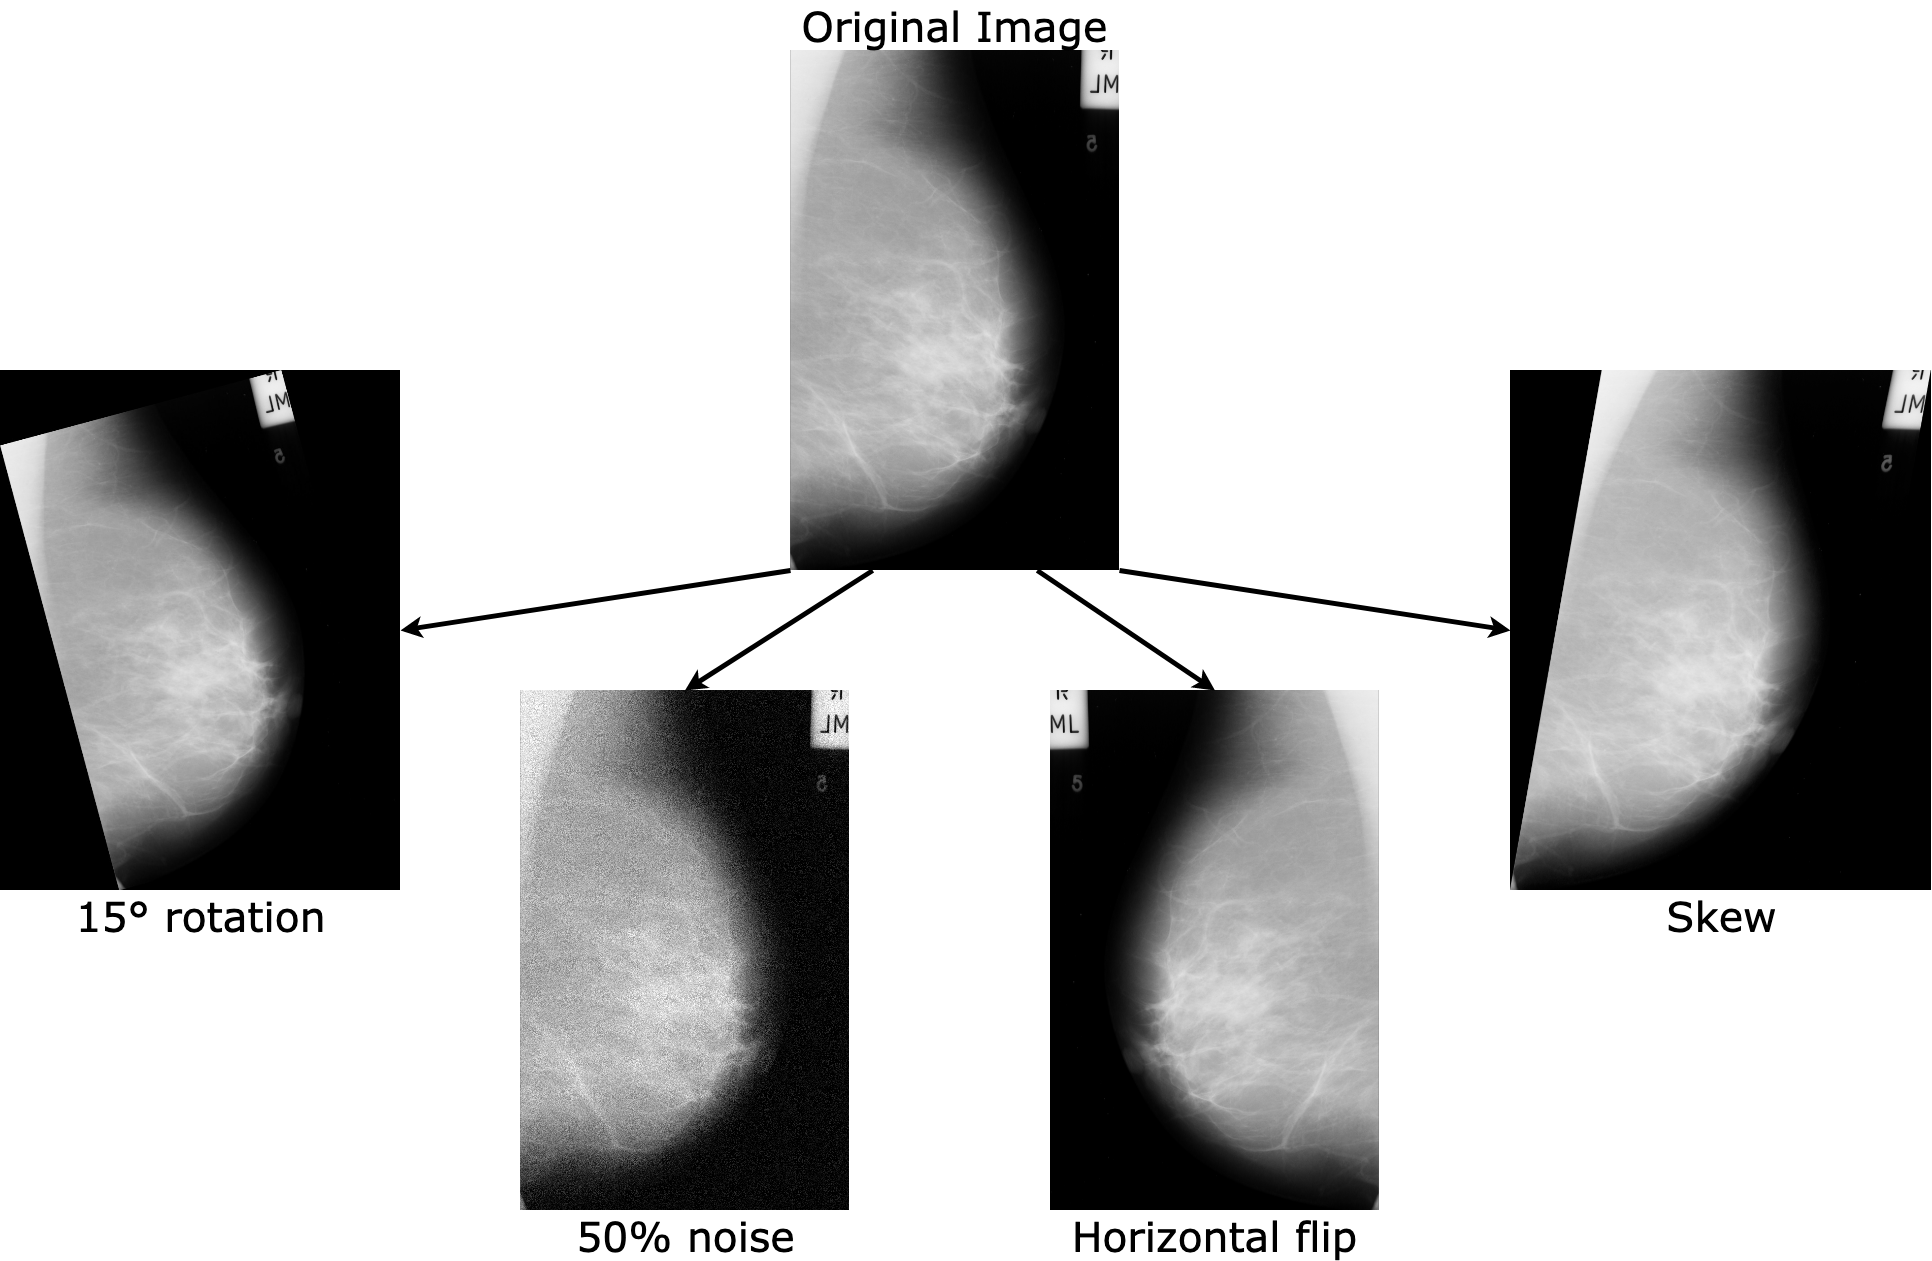
\includegraphics[width=\textwidth]{figures/litsurvey/Data augmentation example.png}}
\caption{\label{fig:litsurvey-Data augmentation example}Example of affine transforms applied to a mammogram to generate new images. Original image retrieved from the mini-MIAS dataset \citep{Suckling1994}, transforms applied in Photoshop and diagram created in Draw.io.}
\end{figure}

\paragraph{Dropout}

Although the previous data augmentation technique can be considered as regularisation as it  helps reduce overfitting, the most common and popular regularisation technique for deep neural networks is dropout. Simply implementing dropout in any CNN has been proven to boost the accuracy by 1 to 2\% \citep{Geron2019} at the cost of training time, even for state-of-the-art neural networks tested on large datasets like ImageNet \citep{Srivastava2014}. Despite training times being increased by 2 to 3 times, the gains in accuracy compensate for the extra time required to train the models implementing dropout.\\

Dropout works by randomly ignoring neurons in any layer (except the output layer) during the forward and backward passes of training, including its input and output connection weights, which helps prevents neurons from co-adapting too much with their neighbours and overfitting the data as they now have to be useful on their own. Essentially, new thinner networks are created at each training step (see Figure~\ref{fig:litsurvey-dropout}), and identical networks will never be sampled in the same training phases as there are $2^N$ possible networks, where $N$ is the number of dropable neurons. The number of neurons dropped in a layer is controlled by the dropout rate hyperparameter $p$, dictating the probability of a neuron being dropped. During testing, the neurons are no longer dropped, and an averaged ensemble of all the thinner trained networks is used. This leads to models that generalise better thanks to neurons that are less sensitive to noise and small changes in the input \citep{Srivastava2014}.

\begin{figure}[ht]
\centerline{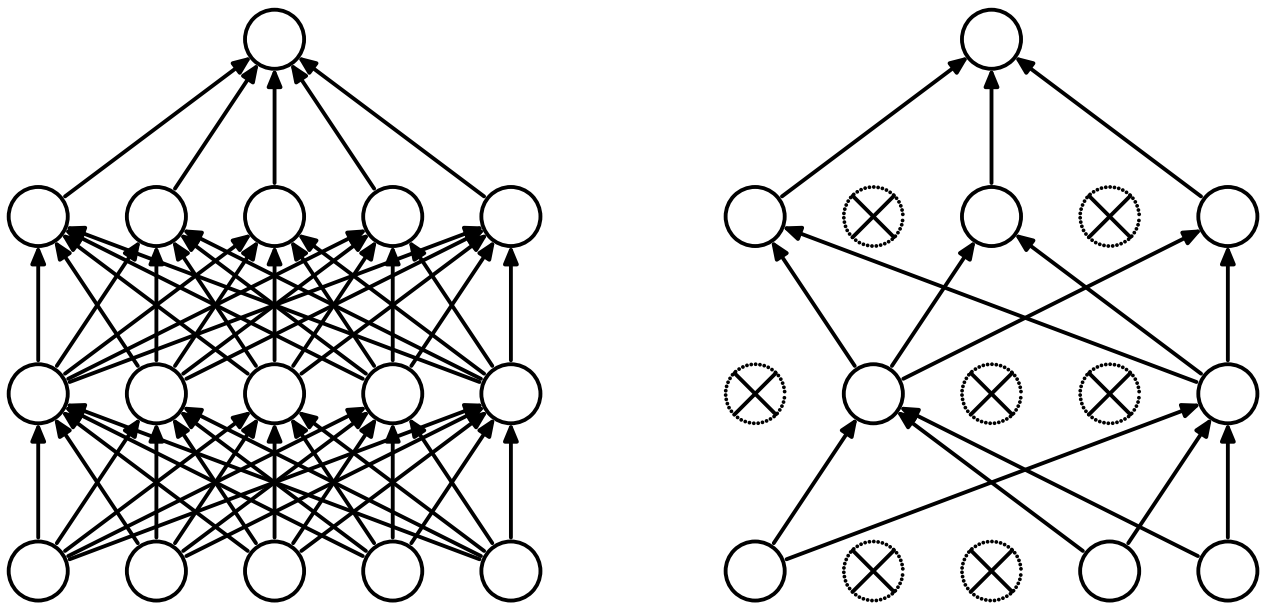
\includegraphics[width=\textwidth]{figures/litsurvey/dropout.png}}
\caption{\label{fig:litsurvey-dropout}Example of standard neural network (left) and a neural network with dropout applied (right). Figure retrieved from Srivastava et al. (2014).}
\end{figure}

\subsubsection{Technological Advances}

The main contributor to the rise of deep learning is linked to the large scale spread and availability of  Graphical Processing Units (GPU) in recent years. GPUs are much more powerful than the general-purpose Central Processing Units (CPU), as they can process large amounts of data in parallel. Initially designed for computer graphics in video games, GPUs are extremely efficient for large-matrix operations, rendering them vital in the field of deep learning \citep{Caulfield2009}. GPU-computing libraries such as CUDA or OpenCL make it possible to use the processing power of GPUs, leading to computing times that are 10 to 30 times faster than CPUs \citep{Litjens2017}.\\

However, GPUs are complicated to use efficiently from a low-level perspective, which is why the collection of open-source software libraries available online is essential for the rise of deep learning. These libraries allow high-level GPU-efficient implementations of the most important deep learning methods and operations, allowing focus to be placed on efficiently implementing deep learning pipelines rather than low-level GPU optimisations \citep{Litjens2017}. The most popular packages nowadays include Tensorflow \citep{tensorflow2015-whitepaper} coupled with Keras \citep{chollet2015keras} and PyTorch \citep{pytorch}.\\

Implementing CNNs entails another drawback linked to the memory requirements (RAM) and the use of GPUs. Indeed, input data, neuron weights and biases all need to be stored in memory as the data propagates through the neural network, especially during training as the data needs to be retained during backpropagation to calculate the error gradients \citep{Geron2019}. For GPU optimisation, this data is formatted as dense vectors for parallel processing optimisations, which can increase local RAM requirements to over 7.5GB for a CNN like ResNet-50 \citep{Hanlon2016}.\\

Without the rise of popularity in GPUs and software libraries to take advantage of the additional processing power offered by GPUs, and the increase in other computing resources such as the amount of GPU and RAM, deep learning would have been successfully applied to fields such as medical imagery analysis nowadays.

%%%%%%%%%%%%%%%%%%%%%%%%%%%%%%%%%%%%%%%%%%%%%%%%%%%%%%%%%%%%%%%%%%%%%%%%%%%%%%%%%%
% SUMMARY
%%%%%%%%%%%%%%%%%%%%%%%%%%%%%%%%%%%%%%%%%%%%%%%%%%%%%%%%%%%%%%%%%%%%%%%%%%%%%%%%%%

\section{Summary}

To complete.

\chapter{Ethics \& Datasets}
\label{ch:chapter-ethics-datasets}
\section{Ethical Considerations}

The deep learning model aimed to be implemented during this project will require real-life data to learn its underlying patterns in order to be able to detect cases of breast cancer in mammograms and to evaluate its performance. Therefore, the main ethical concern when using sensitive medical data such as  mammograms is whether it can be traced back to the original patient. As a result, fully anonymous, open-source and public datasets are used. A full Ethics Application to the University of St Andrew's Teaching and Research Ethics Committee was therefore submitted at the early stages of the project and later approved. The approval letter from the committee can be found in Appendix~\ref{ch:appendix-ethical-approval-letter}.

%%%%%%%%%%%%%%%%%%%%%%%%%%%%%%%%%%%%%%%%%%%%%%%%%%%%%%

\section{Datasets Description}

Three open-sourced anonymised public datasets have been approved by the University of St Andrew's Teaching and Research Ethics Committee for use in this project.

\subsection{DDSM}

todo

\subsection{CBIS-DDSM}

The ``Curated Breast Imaging Subset of DDSM'' (CBIS-DDSM) dataset \citep{Lee2017} is available online from The Cancer Imaging Archive \citep{Clark2013}. The dataset contains a total of 10,239 images in Digital Imaging and Communications in Medicine format (DICOM) gathered from 1,566 patients across 6,775 studies \citep{Lee2017}. This dataset is an updated subset of the older DDSM dataset \citep{DDSMdataset2001}, containing only abnormal cases with benign and malignant tumours (no normal cases).\\

The dataset encloses two different types of mammograms that show different information: calcification VS masses, as well as two different views that are used in most routine mammogram X-ray scans: bilateral craniocaudal (CC) and mediolateral oblique (MLO).

\subsection{mini-MIAS}

The ``mini Mammography Image Analysis Society'' dataset (mini-MIAS) is a smaller dataset of mammograms containing 322 images in greyscale Portable Gray Map (PGM) format with associated ground truth data \citep{Suckling1994} and images all reduced to uniform size of 1024 x 1024 pixels \citep{Vishrutha2014}.

\chapter{Design}
\label{ch:chapter-design}
Based on the machine learning and deep learning applications for the task of breast cancer detection established in Chapter~\ref{ch:chapter-litsurvey}, and the datasets available for this project, design decisions specific to the deep learning pipeline to implement will be covered, along with the reasoning behind the choice of datasets to use and general considerations.

\section{Datasets Decision}

An early design decision taken as a group consisted of electing which datasets to use, as Chapter~\ref{ch:chapter-ethics-datasets} revealed that each dataset has different characteristics. Despite being widely used in existing literature (see Chapter~\ref{ch:chapter-litsurvey}), popular feature-based datasets containing extracted mammogram data such as the WBCD dataset \citep{Wolberg1995} will not be used as the objective of using deep learning models such as CNNs is to learn which features to extract by using the raw image in 2D space rather than data flattened into 1D arrays. If extracted features such as the ones from WBCD were used, then already successful machine learning algorithms such as SVMs or DTs could be used instead of deep learning techniques.\\

From a clinical point of view, the mini-MIAS dataset is interesting as it contains both abnormal cases and normal cases as well, resulting in three classes (normal, benign and malignant cases). Its smaller size makes it useful for initial prototyping but has the downside of requiring more image processing techniques such as data augmentation to generate enough data to feed into the deep learning model. The different types of breast backgrounds (see Section~\ref{sec:ethics-mini-MIAS-dataset-description}) is not considered during training to avoid further splitting the dataset.\\

The CBIS-DDSM dataset was chosen over the DDSM dataset as it is an updated version of the older DDSM dataset, and is curated by a trained mammographer. Additionally, it uses uncompressed images in DICOM format rather than LJPEG format, which is deprecated nowadays, resulting in much higher quality imagery; and is already split into training/testing sets, allowing for accurate performance comparisons with other papers using the same dataset. Indeed, the large uncompressed format offered by DICOM means that the mammograms can be fed into the CNN with larger sizes, allowing the model to potentially learn more low-level features. Despite the CBIS-DDSM dataset containing two different views (CC and MLO), the mammograms in each case are treated as separate individual images due to the limited number of samples available.\\

%%%%%%%%%%%%%%%%%%%%%%%%%%%%%%%%%%%%%%%%%%%%%%%%%%%%%%%%%%%%%%%%%%%%
%%%%%%%%%%%%%%%%%%%%%%%%%%%%%%%%%%%%%%%%%%%%%%%%%%%%%%%%%%%%%%%%%%%%
%%%%%%%%%%%%%%%%%%%%%%%%%%%%%%%%%%%%%%%%%%%%%%%%%%%%%%%%%%%%%%%%%%%%

\section{Deep Learning Pipeline Design Analysis}

The deep learning pipeline implemented for the task of breast cancer detection can be broken down in four distinct phases condensed in Figure~\ref{fig:design-flowchart}:

\begin{itemize}
    \item \textbf{Data pre-processing}: loading a dataset in memory and processing it to gather the pair of images and labels for the classification task.
    \item \textbf{Model training}: creating a CNN model that can fit the data to learn the training set samples. Predictions are carried out once the model finished training on the validation and test sets.
    \item \textbf{Result visualisation}: The model's performance is evaluated by calculating various metrics and plotting predictions.
\end{itemize}

\begin{figure}[ht]
\centerline{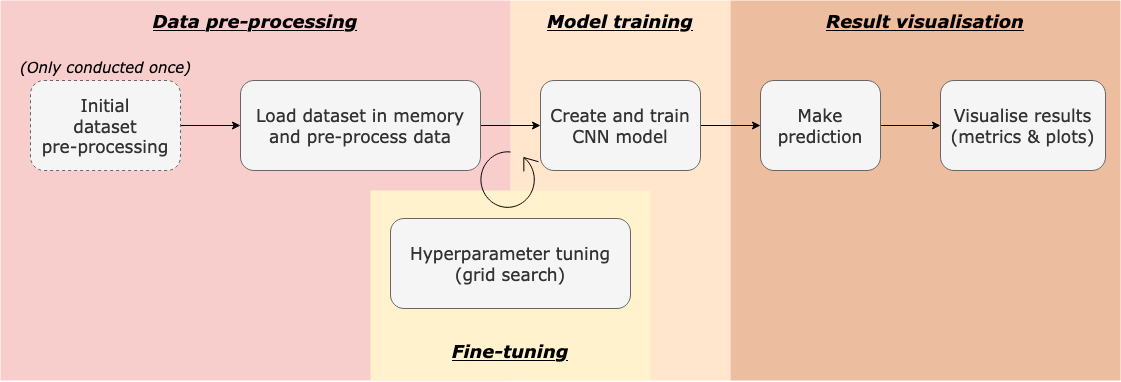
\includegraphics[width=\textwidth]{figures/design/design flowchart.png}}
\caption{\label{fig:design-flowchart}A high-level flowchart of the breast cancer detection deep learning pipeline to implement, separated between data pre-processing, model training, results visualisation and fine-tuning.}
\end{figure}

%%%%%%%%%%%%%%%%%%%%

\subsection{Data pre-processing}

\subsubsection{Dataset balance}
\label{sec:design-dataset-balance}

As this is a classification task, it is essential to visualise the distribution of classes in the datasets to determine whether the data balance is skewed or not (whether some classes are much more frequent than other classes \citep{Geron2019}). The class distributions are plotted in Figure~\ref{fig:design-datasets-balance}.

\begin{figure}[h]
\centering
\begin{subfigure}{.5\textwidth}
  \centering
  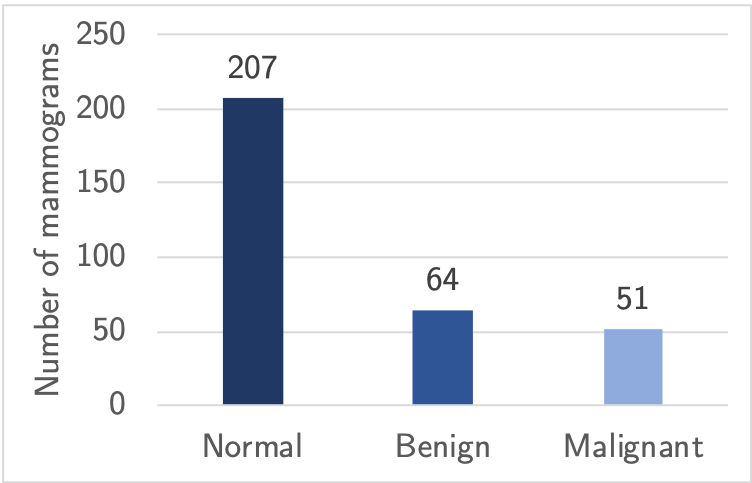
\includegraphics[width=0.94\textwidth]{figures/design/mini-mias-balance.png}
  \caption{mini-MIAS class distribution.}
  \label{fig:design-mini-mias-balance}
\end{subfigure}%
\begin{subfigure}{.5\textwidth}
  \centering
  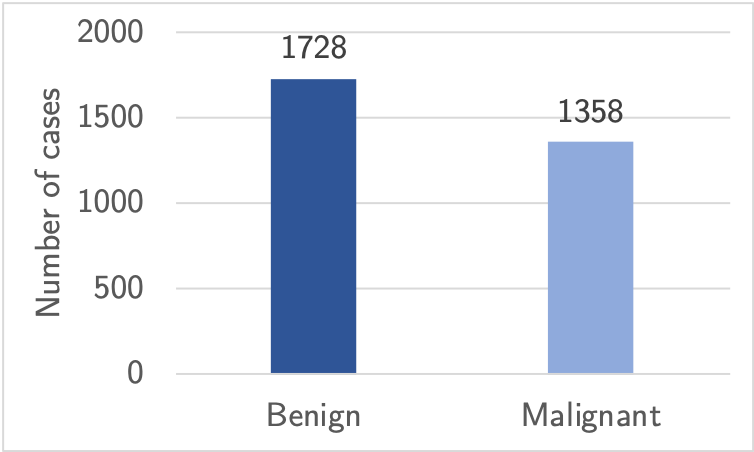
\includegraphics[width=\textwidth]{figures/design/cbis-ddsm-balance.png}
  \caption{CBIS-DDSM class distribution.}
  \label{fig:cbis-ddsm-balance}
\end{subfigure}
\caption{\label{fig:design-datasets-balance}Class distribution for the mini-MIAS and the CBIS-DDSM datasets.}
\end{figure}

These bar charts reveal that the mini-MIAS dataset is heavily imbalanced as the distribution is not uniform, which must be taken into account to avoid training a biased CNN model. Potential solutions to counter this imbalance would be to either:
\begin{itemize}
    \item \textit{undersample} the dataset by dropping images altogether;
    \item \textit{oversample} the dataset, which can be achieved via data augmentation,
    \item include \textit{class weights} to give more importance to under-represented classes. 
    %https://datascience.stackexchange.com/questions/13490/how-to-set-class-weights-for-imbalanced-classes-in-keras 
    %https://www.tensorflow.org/tutorials/structured_data/imbalanced_data#class_weights
\end{itemize}

Undersampling the dataset can be considered as inefficient as it will diminish the number of samples the model could learn from by dropping samples from the majority class \citep{Liu2009}. As the datasets are already very small (maximum of 10,239 images in CBIS-DDSM), undersampling would be a poor strategy as it may discard useful features that could be learned. Consequently, oversampling by creating new artificial images resembling the original data is a viable solution as it was proven to increase accuracies (see Section~\ref{sec:litsurvey-data-augmentation}). Alternatively, a cheaper option in terms of computing power that does not require the dataset to be touched would be to add class weights, which will cause the loss to become a weighted average giving more importance to less frequent classes \citep{Zhu2018}.

\subsubsection{Dataset split}

The dataset is immediately split between a training and a testing set to avoid any form of data snooping, which corresponds to the poor practice of making design decisions (either voluntary or involuntary) after having viewed the data and detecting patterns that could lead to favouring certain models or hyperparameters above others. Due to the small size of the datasets used and to avoid causing further imbalance to the datasets, the splits are not randomly sampled. Instead, stratified sampling is used, which consists of maintaining representative samples from the data in both the training and the testing sets to avoid introducing sampling bias.\\

An 80\%/20\% split, often used in machine learning and seen in breast cancer detection papers \citep{Yue2018}, is used to split the mini-MIAS dataset. The CBIS-DDSM does not need to be manually divided as it was already split with the appropriate stratification when it was built \citep{Lee2017}.\\

After this step, only the training set is considered until the final results evaluations, while the testing set is set aside and forgotten about. The assumption that the data never changes during the development of the project is made, as not using the random generator with a fixed seed would cause different samples to be extracted into the training and testing sets, thus neglecting the results. 

\subsubsection{Data loading}

The mini-MIAS dataset is very small in size (339 Mb before pre-processing, 202 Mb after pre-processing), containing only 322 images. It can therefore be loaded into memory without any data loading optimisation techniques. However, the CBIS-DDSM dataset is much larger, containing 10,239 images that cover 163.6 Gb of disk space. The dataset therefore cannot be loaded in memory in a single import and needs to be loaded in batches to be fed into the CNN sequentially. % mention batches and caching

\subsubsection{Data normalisation}

Images are resized to a target size during import to scale them down (CBIS-DDSM images are larger than 3000 x 5000 pixels)  and to avoid having inconsistent inputs. Observing the pixel intensities of the images found in the datasets reveal that they correspond to integers ranging from 0 to 255. However, because the weights in neural networks are small, having such large input values can disrupt and slow down the training process, ultimately leading to lower accuracies. Therefore, normalising the pixel intensities to values in the range of 0 to 1 can help fight this problem by ensuring all values are small. An example of the pixel values before and after normalisation can be seen in Figure~\ref{fig:design-Normalisation example}.

\begin{figure}[ht]
\centerline{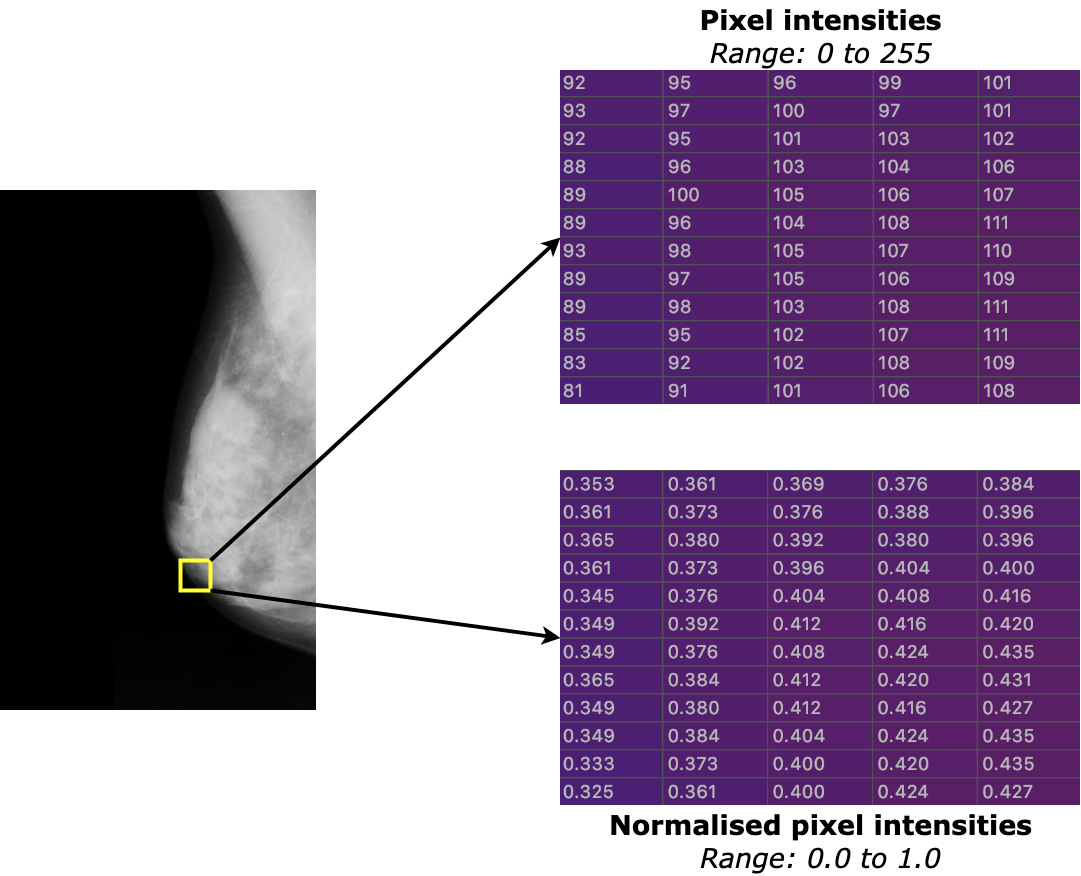
\includegraphics[width=0.9\textwidth]{figures/design/Normalisation example.png}}
\caption{\label{fig:design-Normalisation example}Example of the pixels values that make up a mammogram before and after normalisation.}
\end{figure}

\subsubsection{Label encoding}

As the labels for each mammogram are in categorical string format, they must be encoded into a numerical format. On the one hand, due to the sparse nature of the labels (only three categories), one-hot encoding is chosen for the mini-MIAS dataset, where a single digit may have the value 1 while the others remain at value 0 to tell apart the different labels. The one-hot encodings of the labels can be seen in Table~\ref{tab:one-hot-encoding-example}.

% The data must be fed to the neural network in binary form. One-hot encoding is therefore chosen as it suits the sparse representation of the data, which is made up of only five target categories. Only a single digit may have the value 1 in one-hot encoding, while the others remain at value 0 \cite{lec16}. The one-hot encodings of the target categories can be seen in Figure \ref{fig:one_hot_encoding}.

\begin{table}[h]
\centering
\begin{tabular}{|c|c|}
\hline
\textbf{Categorical format} & \textbf{One-hot encoding} \\ \hline
\textit{Normal}             & 1 0 0            \\ \hline
\textit{Benign}             & 0 1 0            \\ \hline
\textit{Malignant}          & 0 0 1            \\ \hline
\end{tabular}
\caption{Conversion from string (categorical) format to one-hot encoding.}
\label{tab:one-hot-encoding-example}
\end{table}

On the other hand, in the case of binary datasets like CBIS-DDSM, binary encoding can be used instead of one-hot encoding, as seen in Table~\ref{tab:binary-encoding-example}.

\begin{table}[h]
\centering
\begin{tabular}{|c|c|}
\hline
\textbf{Categorical format} & \textbf{Binary encoding} \\ \hline
\textit{Benign}             & 0                        \\ \hline
\textit{Malignant}          & 1                        \\ \hline
\end{tabular}
\caption{Conversion from string (categorical) format to binary encoding.}
\label{tab:binary-encoding-example}
\end{table}

%%%%%%%%%%%%%%%%%%%%

\subsection{Model training}

At this stage, the training data is ready to be fed into the CNN model. The classification models will learn the processed images from the training set loaded in memory before making their predictions, which will be compared with the ground truth labels for evaluation.

\subsubsection{CNN model}
\label{sec:design-cnn-model-decision}

Due to the small nature of the CBIS-DDSM and mini-MIAS datasets used, state-of-the-art CNN models pre-trained on large general datasets like ImageNet are used rather than creating a CNN from scratch, a technique known as transfer learning that is proven to work on breast cancer detection tasks \citep{Shen2017, Falconi2019}.\\

Different CNN architectures can be used as the base of a custom CNN model tailored for breast cancer detection. This is achieved by using popular CNN architectures available with Keras such as VGG19, ResNet50, InceptionV3, DenseNet121 and MobileNetV2 as the base of the CNN \citep{kerasApplications}. The fully connected layers of these models, which are designed for general classification of natural images into 1,000 different categories \citep{Krizhevsky2012}, are dropped from the model and replaced with a custom MLP. The fully-connected MLP contains hidden layers and an output layer with different activation functions based on the dataset used.\\

If large images are used, then additional convolutional and spooling layers are added before the base model to downsample the image to smaller sizes and learn low-level features, followed by the pre-trained base model, a flatten layer to convert the output from 2D to 1D, and finally the MLP which will make the final prediction. Dropout layers are added in the MLP to avoid over-fitting.

\begin{figure}[ht]
\centerline{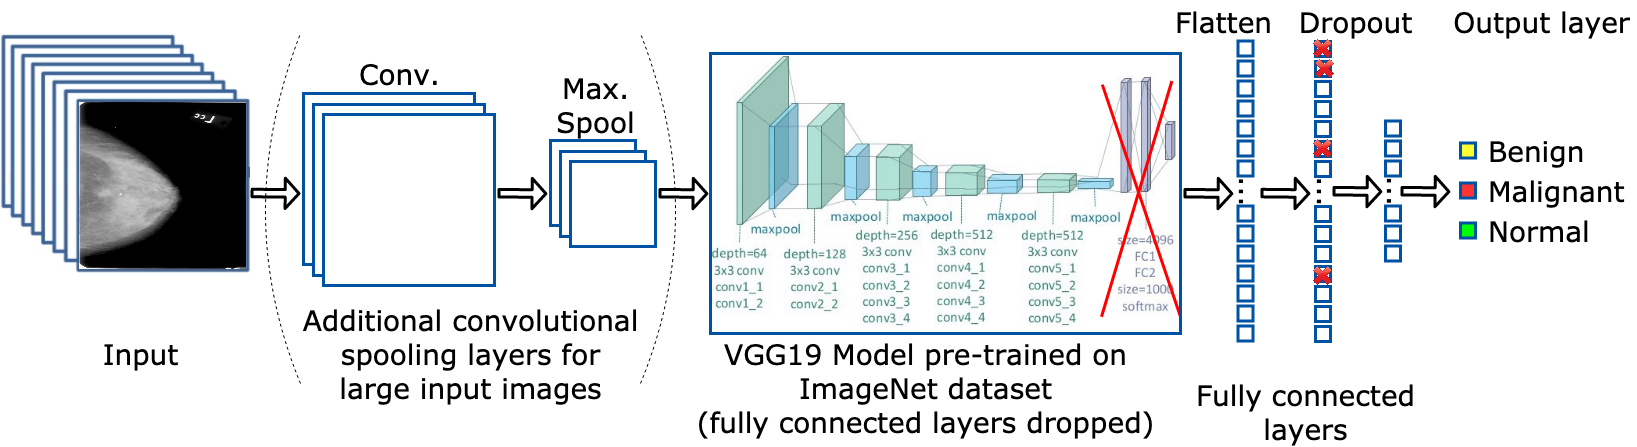
\includegraphics[width=1.1\textwidth]{figures/design/CNN architecture.png}}
\caption{\label{fig:design-CNN architecture}CNN architecture used. VGG19 image retrieved from \url{https://tinyurl.com/rpp49oc}.}
\end{figure}

\subsubsection{Model fitting}

\paragraph{Activation functions}

Different activation functions can be used in the output layer of the CNN (see Figure~\ref{fig:design-activation functions}). Typically, a single neuron with a sigmoid activation function is used for binary problems as it outputs an independent value between 0 and 1 that can be interpreted as a probability of the positive class. Inversely, a softmax activation function transforms the output of the last hidden layer into probabilities for each class that sum up to 1. These probabilities are dependent of each other, as each sample must belong to one class only, making it perfect for multi-class classification of breast mammograms (each sample can only be either normal, benign or malignant, so to increase the probability of one class, it must decrease it for another).

\begin{figure}[ht]
\centerline{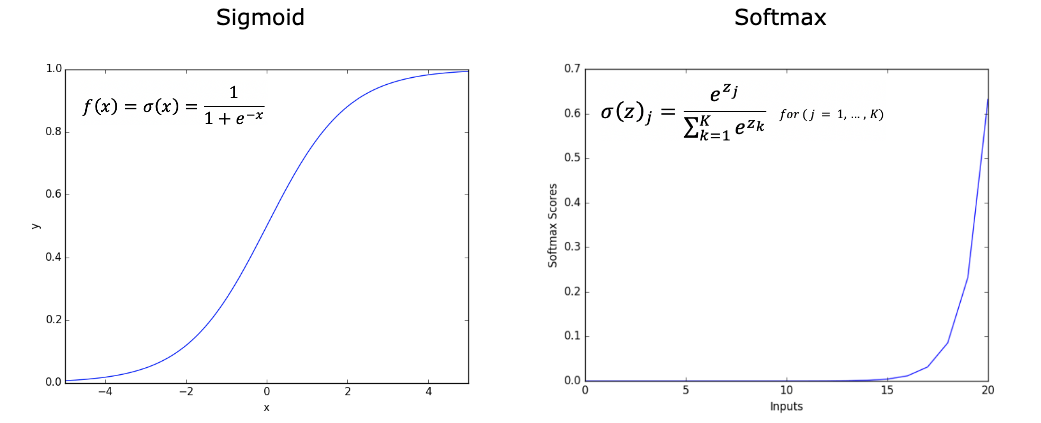
\includegraphics[width=1.1\textwidth]{figures/design/activation functions.png}}
\caption{\label{fig:design-activation functions}Visualisation of the sigmoid and softmax activation functions.}
\end{figure}
% https://glassboxmedicine.com/2019/05/26/classification-sigmoid-vs-softmax/

Therefore, the output layer will use a sigmoid with the CBIS-DDSM dataset, and a softmax with the mini-MIAS dataset.

\paragraph{Loss function}

Cross entropy is one of the most commonly used loss functions as it can be used for both binary and multi-class tasks \citep{Litjens2017}. Because probabilities are being estimated through the sigmoid and softmax activation functions, cross entropy is the ideal loss function as it heavily penalises the model when a low probability is predicted for the target class \citep{Geron2019}.
% https://www.machinecurve.com/index.php/2019/10/22/how-to-use-binary-categorical-crossentropy-with-keras/
%https://gombru.github.io/2018/05/23/cross_entropy_loss/

\paragraph{Optimiser}

Due to the deep nature of the model, it is important to minimise the number of hyperparameters to control. Adaptive learning rate algorithms usually generalise better than traditional optimisers like Stochastic Gradient Descent (SGD) or momentum, which are slow to converge and require more fine-tuning. The most general adaptive optimiser is \textit{adaptive moment estimation} (Adam), which combines both momentum for more significant steps in the direction of the steepest gradient and Root Mean Square Prop (RMSProp) for accelerating more on steep slopes than small slopes, making it the best choice for this model.
%https://towardsdatascience.com/full-review-on-optimizing-neural-network-training-with-optimizer-9c1acc4dbe78

\paragraph{Transfer learning}
\label{sec:design-transfer-learning-training-phase}

To best make use of the transfer learning technique with the base model's weights instantiated using ImageNet weights, training is separated into two phases:
\begin{enumerate}
    \item All the layers from the base model are frozen, enabling only the custom MLP with fully connected layers to fit the mammogram images. The initial training phase ends once the maximum number of epochs is reached, or the early stopping condition is met.
    \item All the layers are unfrozen, and training is resumed with a smaller learning rate $\alpha = 0.00001$, allowing the base model to slightly alter its weights to adapt to the mammogram dataset while not forgetting the ImageNet knowledge.
\end{enumerate}

\paragraph{Validation set \& early stopping}
\label{sec:design-validation-early-stopping}

To ensure that the model generalises well to unseen  data from the testing set, the training set is further split to form a validation set using a 75\%25\% split on training set; resulting in a 60\%/20\%/20\% of the full dataset. The validation set is used to make predictions at the end of each epoch by calculating the loss and accuracy. These values are then monitored to stop the training before the maximum number of epochs is reached if the validation accuracy or loss do not improve after a certain number of epochs, preventing the model from overfitting the data too much.\\

Due to time constraints, k-fold cross-validation, which divides the training set into $K$ subsets and evaluates the model $K$ times, cannot be used as training the model on the CBIS-DDSM dataset can take anywhere from 1h15m to 8h49 (see Chapter~\ref{ch:chapter-evaluation}), which would be multiplied by a factor of $K$. Therefore, a validation set is used instead.

\paragraph{Fine-tuning}
\label{sec:design-fine-tuning-bagoftricks}

Traditionally, a grid search approach would have been preferred to fine-tune the model's hyperparameters. However, due to the significant training runtime and the number of hyperparameters to fine-tune, a grid search would have been unrealistic given the time frame of the project. Additionally, two attempts at implementing grid search were unsuccessful, as a known bug on the Keras wrapper for Scikit-Learn prevented the use of the \textit{GridSearch class}, and Optuna was incompatible with the current version of Tensorflow I/O being used.\\

Instead, a bag-of-tricks approach is selected, manually trying different deep learning techniques mentioned in this chapter such as using different pre-trained CNN models, amounts of transfer learning, amounts of data augmentation, dropout values, input image sizes.
% over a genetic algorithm to naturally find best hyperparameters.

%%%%%%%%%%%%%%%%%%%%

\subsection{Result visualisation}
\label{sec:design-results-visualisation}

The following terminology is used to define the metrics used below:
\begin{itemize}
    \item TP: True Positives (positive case correctly predicted as positive);
    \item TN: True Negatives (negative case correctly predicted as negative);
    \item FP: False Positives (negative case incorrectly predicted as positive);
    \item FN: False Negatives (positive case incorrectly predicted as negative).
\end{itemize}

\subsubsection{Overall accuracy}

The imbalanced class distributions (see Section~\ref{sec:design-dataset-balance}) must be taken into account when analysing the classifiers' scores. Indeed, using an evaluation metric such as overall accuracy (see Equation~\ref{eq:accuracy}, \cite{Falconi2019}) would be misleading as it would not be representative of how well the classifier fitted the data.

\begin{equation}
\label{eq:accuracy}
    Accuracy = \frac{TP + TN}{P + N}
\end{equation}

For instance, if a dumb classifier that always classifies an image as ``normal'' is created, it would achieve 64.28\% accuracy on the mini-MIAS dataset despite  never picking up abnormal cases. Therefore, a mixture of additional metrics should be used to assess how well the model learns the mammograms data and generalises to unseen cases.

\subsubsection{Precision \& Recall}

Precision corresponds to the number of correct positive predictions (see Equation~\ref{eq:precision}, CITE), showing the model's ability to avoid labelling negative instances as positive. 

\begin{equation}
\label{eq:precision}
    Precision = \frac{TP}{TP+FP}
\end{equation}

Recall is the number of positive instances that are correctly predicted (see Equation~\ref{eq:recall}, CITE), showing how well the model can find all positive instances.

\begin{equation}
\label{eq:recall}
    Recall = \frac{TP}{TP+FN}
\end{equation}

\subsubsection{F1 Score}

Together, precision and recall can be combined into a more concise metric, the \textit{F1 score}, which corresponds to the harmonic mean of precision and recall (see Equation \ref{eq:f1-score}). To achieve a high F1 score, both precision and recall must be high (unlike a regular mean) because as the precision goes down, the recall goes up, and vice versa, making the F1 score a reliable metric for evaluating a classifier since a balance between precision and recall must be found \citep{Geron2019}.

\begin{equation}
\label{eq:f1-score}
    F_{1} = \frac{2}{\frac{1}{precision} + \frac{1}{recall}} = \frac{TP}{TP+\frac{FN + FP}{2}}
\end{equation}

\subsubsection{Confusion matrix} 

This visual metric plots the number of predictions made for each class for each possible class in a table, with each row corresponding to the actual labels and each column corresponding to a prediction. It is beneficial for detecting which actual classes are being detected the most, and what predicted classes are misclassified as. To further highlight the misclassifications and compare predictions with other classifiers, the confusion matrices are normalised to show a percentage rather than a count \citep{Geron2019}.

%%%%%%%%%%%%%%%%%%%%%%%%%%%%%%%%%%%%%%%%%%%%%%%%%%%%%%%%%%%%%%%%%%%%
%%%%%%%%%%%%%%%%%%%%%%%%%%%%%%%%%%%%%%%%%%%%%%%%%%%%%%%%%%%%%%%%%%%%
%%%%%%%%%%%%%%%%%%%%%%%%%%%%%%%%%%%%%%%%%%%%%%%%%%%%%%%%%%%%%%%%%%%%

\section{General Design Decisions}

\subsection{Programming Language}

% Choosing a programming language is one of the most essential aspects to take into account as it is the medium used to transform the system from design to implementation. However, choosing from over 250 different programming languages \citep{tiobe} can be tricky, which is why multiple views have to be evaluated before choosing a programming language. Four popular programming languages are considered for this project: Python, Java, R and  Javascript.\\
% https://becominghuman.ai/best-languages-for-machine-learning-in-2020-6034732dd242

The first element to consider when choosing a programming language is the availability of third-party libraries used for implementing common machine learning functionalities, as well as data pre-processing, manipulation and visualisation techniques found in deep learning systems to avoid manually implementing them. The most commonly used machine learning libraries nowadays are all available in Python \citep{raschka2017python}, including SciKit-Learn \citep{scikit-learn}, Pandas \citep{reback2020pandas}, Matplotlib \citep{Hunter:2007}, NumPy \citep{numpy} and Seaborn \citep{seaborn}. In terms of deep learning libraries, Tensorflow (available in Python, R and Javascript) and PyTorch (available in Python) are  the most popular ones (Appendix~\ref{sec:appendix-keras_vs_pytorch}).\\

In terms of speed, compiled languages are quicker than interpreted languages, but because the main bottleneck in a deep learning system is the training phase of the model, which mainly relies on the library used rather than the language itself, speed is not taken into account. Finally, of all the programming languages mentioned, Python is the favoured one in terms of personal preference, familiarity, and experience, especially when applied to machine learning projects, making it the apparent programming language candidate for this project. For a complete review of the main pros and cons considered between when deciding between Python, Java, R and Javascript, refer to Appendix~\ref{sec:appendix-programming-languages-comparison}.

\subsection{Deep Learning Framework}

Due to the vast nature of the datasets and complexity of the deep learning models to implement, powerful computing resources will be used in the form of Graphical Processing Units (GPU). A GeForce GTX 1060 6GB is provided by the School of Computer Science and remotely accessed via SSH to a lab machine equipped with the GPU in question running on CentOS.\\

To make use of the GPU's computing capabilities, deep learning frameworks with CUDA support (for parallel computing and GPU optimisations), CNN support and pre-trained models should be used. The two most popular deep learning frameworks nowadays are Tensorflow coupled with Keras, and PyTorch. Tensorflow/Keras being relatively older than PyTorch, have got more online support, which is confirmed by the number of daily downloads Keras has compared to PyTorch (ten times more), as well as the number of mentions in academic papers (see figures  in Appendix~\ref{sec:appendix-keras_vs_pytorch}), making them the selected deep learning library.

\subsection{Interface}

A Command-Line Interface (CLI) is selected, allowing arguments and flags to be passed to execute different sections of the code. Arguments control the dataset to use, the CNN model, and the mode to run in (training or testing). Flags control the verbose mode to print more statements in the terminal for debugging purposes. The full set of instructions to run the code can be found in Appendix~\ref{ch:appendix-usage-instructions}.

%%%%%%%%%%%%%%%%%%%%%%%%%%%%%%%%%%%%%%%%%%%%%%%%%%%%%%%%%%%%%%%%%%%%
%%%%%%%%%%%%%%%%%%%%%%%%%%%%%%%%%%%%%%%%%%%%%%%%%%%%%%%%%%%%%%%%%%%%
%%%%%%%%%%%%%%%%%%%%%%%%%%%%%%%%%%%%%%%%%%%%%%%%%%%%%%%%%%%%%%%%%%%%

\section{Design Decisions Summary}

\begin{enumerate}
    \item Datasets:
    \begin{itemize}
        \item CBIS-DDSM (binary classification)
        \item mini-MIAS (multi-class classification)
    \end{itemize}
    
    \item Data pre-processing steps:
    \begin{itemize}
        \item 60/20/20\% train/test/validation splits
        \item Data augmentation
        \item Image normalisation
        \item One-hot encoding (CBIS-DDSM) and binary encoding (mini-MIAS)
    \end{itemize}
    
    \item Model training:
     \begin{enumerate}
        \item Base model: VGG19, ResNet50, InceptionV3, DenseNet121 and MobileNetV2 
        \item Output layer activation function: softmax (CBIS-DDSM) and sigmoid (mini-MIAS)
        \item Optimiser: Adam
        \item Loss function: Cross entropy
        \item Transfer learning
        \item Generalisation to unseen data: validation loss and accuracy early stopping
        \item Fine-tuning: bag-of-tricks approach
    \end{enumerate}
    
    \item Evaluation Metrics:
    \begin{enumerate}
        \item Numerical metrics:
        \begin{itemize}
            \item Overall accuracy
            \item Precision \& recall
            \item F1 score
        \end{itemize}
        \item Visual metrics:
        \begin{itemize}
            \item Confusion matrices (counts)
            \item Normalised confusion matrices
        \end{itemize}
    \end{enumerate}
    
    \item Programming language:
    \begin{enumerate}
        \item Python 3.7
        \item Open-source frameworks:
        \begin{itemize}
            \item Tensorflow \& Keras
            \item Scikit-Learn
            \item NumPy, Pandas, MatplotLib \& Seaborn
        \end{itemize}
    \end{enumerate}
    
    \item Interface: Command-Line Interface
\end{enumerate}


\chapter{Implementation}
\label{ch:chapter-implementation}
The implementation of the breast cancer detection system was conducted in two parts. The first part corresponds to a common pipeline developed in group, and the second part to individual implementations using the common pipeline as a baseline. The distribution of work during the implementation of the common pipeline can be found in Appendix~\ref{ch:appendix-team-meeting-summaries}.

%%%%%%%%%%%%%%%%%%%%%%%%%%%%%%%%%%%%%%%%%%%%%
%%%%%%%%%%%%%%%%%%%%%%%%%%%%%%%%%%%%%%%%%%%%%
%%%%%%%%%%%%%%%%%%%%%%%%%%%%%%%%%%%%%%%%%%%%%

\section{Code Design}

The code is designed by splitting essential code into functions spread across multiple python modules, which are all organised into different directories based on what task they accomplish.

The entry point is in the ``main.py'' module, which parses command line arguments used to execute different parts (e.g. which dataset to use). It contains the main flow of execution with calls to functions for processing the data, creating the CNN models and evaluating the results.\\

Functions linked to data pre-processing, such as retrieving image paths and labels, processing images, encoding labels, loading the data into memory and transforming images for data augmentation, are all located in the \textit{data\_operations} directory. One-time scripts for parsing the images' paths and labels for each dataset are in the \textit{dataset\_processing\_scripts} directory.\\

All CNN-related code, such as creating the model, compiling it, fitting, making predictions or evaluating it is placed in a custom \textit{CNN\_Model} class, which can be found in the \textit{cnn\_models.py} module. Separate models, such as VGG or InceptionV3, are individually placed the \textit{cnn\_models} directory.\\

Functions handling result visualisations in the form of plots and CSV reports are all situated in the \textit{data\_visualisation} directory.\\

General functions for printing information in the terminal and common operations are all located in the \textit{utils.py} module, while global command line arguments used throughout the code are all stored in the \textit{config.py} module.


%%%%%%%%%%%%%%%%%%%%%%%%%%%%%%%%%%%%%%%%%%%%%
%%%%%%%%%%%%%%%%%%%%%%%%%%%%%%%%%%%%%%%%%%%%%
%%%%%%%%%%%%%%%%%%%%%%%%%%%%%%%%%%%%%%%%%%%%%

\section{Common Deep Learning Pipeline}

A detailed flowchart of the deep learning pipeline implemented can be found in  Figure~\ref{fig:implementation-detailed-flowchart}.

\begin{figure}[ht]
\centerline{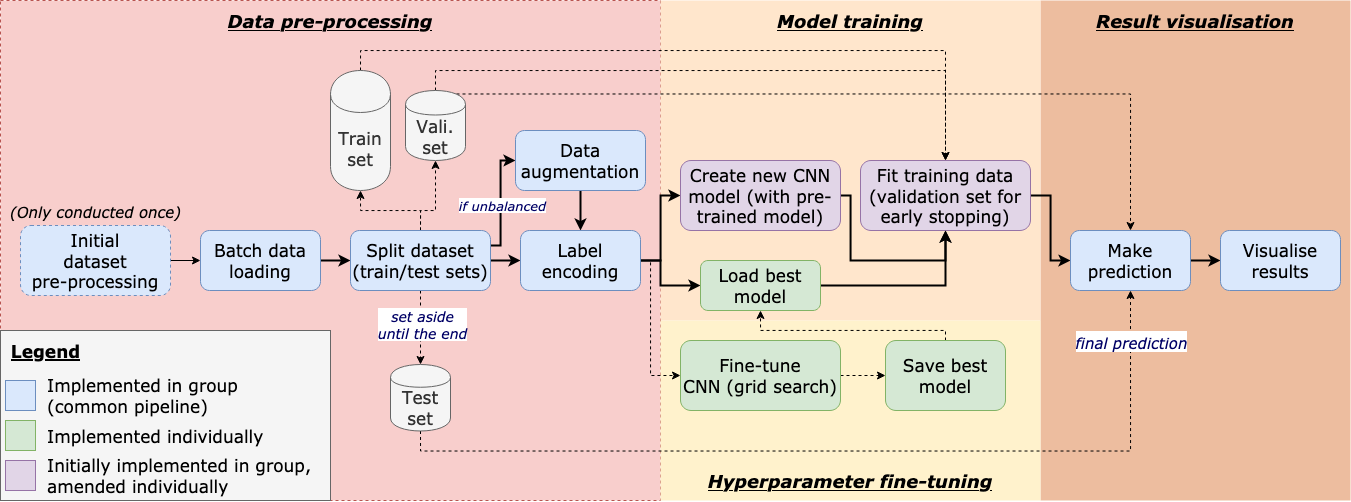
\includegraphics[width=1.25\textwidth]{figures/implementation/detailed flowchart.png}}
\caption{\label{fig:implementation-detailed-flowchart}Flowchart. Created using draw.io.}
\end{figure}

%%%%%%%%%%%%%%%%%%%%%%%%%%%%%%%%%%%%%%%%%%%%%

\subsection{Data pre-processing}

\subsubsection{Initial dataset processing}

Two Python scripts written to initially parse CSV files mapping image paths and their labels in order to reorganise the images in labelled folders for classification.\\

File formats: PGM and DICOM files converted to arrays to be readable by the CNNs as input.\\

%%%%%%%%%%%

\subsubsection{Data loading}

Processed CSV files containing image paths are parsed to generate a list of all images and a list of all labels.\\

Tensorflow cache and batch functions used to load the CBIS-DDSM dataset.\\

No optimisations used for the smaller mini-MIAS dataset (just the Keras \textit{img\_to\_array} and \textit{load\_img} functions).\\

%%%%%%%%%%%

\subsubsection{Image processing}

For mini-MIAS, images are loaded, resized to a target size (1024x1024 or 224x224 pixels), converted to an array format and normalised.\\

Images resized on import to match the input size of the pre-trained model. For instance, VGG19 takes 224x224px images.\\

Normalising images to fit in [0-1] float range rather than [0-255] integer range.\\

Scikit-Learn's \textit{LabelEncoder} class is used to one-hot encode labels and Keras' \textit{to\_categorical}  function is used to convert to a binary class matrix usable by the CNN models.\\

A 60/20/20\% shuffled stratified split (maintain class balance across split sets) is used for the mini-MIAS dataset. A default 80/20\% train test split is already done for CBIS-DDSM dataset, and the training set is further split into 75/25\% for a total 60/20/20\% split.\\

Class weights are calculated automatically using sklearn's \textit{class\_weight}.\\

For the mini-MIAS dataset, images are cropped around a ROI (Region of Interest) sized 224x224 pixels if there is one, otherwise around a 224x224 region around the centre of the image.\\

Data augmentation for the mini-MIAS  dataset images to balance the class distribution. Rotations, noise, shears and rotation flips are randomly added to existing images to create new images and to balance classes. These are then shuffled to ensure that newly generated images are not grouped together.

%%%%%%%%%%%%%%%%%%%%%%%%%%%%%%%%%%%%%%%%%%%%%

\subsection{Model training}

A VGG19 pre-trained model (using ImageNet weights) is used through the Keras API. The fully connected layers are replaced with new fully connected layers to accommodate the breast cancer detection classes (benign and malignant for CBIS-DDSM, and normal as well for mini-MIAS).\\

Training is conducted in two phases:
\begin{itemize}
    \item During the first phase, the VGG19 layers are frozen (weights are not updated during training) and only the fully connected layers are being updated. This is done by setting the \textit{trainable} attribute for the layers in question to False.
    \item Once the first training phase is stopped (using early stopping when the validation loss does not improve after 8 epochs), all the layers are unfrozen and training is resumed at a lower learning rate for the VGG19 models to adapt to the mammograms images.
\end{itemize}

Additional convolution and spooling layers are added before the pre-trained model to accommodate larger images. These are slowly reduced in size as they go through the spooling layers, allowing lower-level features to be learned before passing through the VGG19 model.\\

Once the CNN model is finished training model is saved in HDF5 format in order to save the model's architecture, the layers' hyperparameters, all the connection weights and biases that were learned during training \citep{Geron2019} and the optimiser used.

%%%%%%%%%%%%%%%%%%%%%%%%%%%%%%%%%%%%%%%%%%%%%

\subsection{Results visualisation}

Scikit-Learn's \textit{classification\_report} and \textit{accuracy\_score} functions used to get numerical result metrics.\\

Matplotlib used to plot the ROC curve and seaborn for the confusion matrices.

%%%%%%%%%%%%%%%%%%%%%%%%%%%%%%%%%%%%%%%%%%%%%

\subsection{General}

Python's \textit{argparse} is used to implement the CLI application, accepting different arguments such as the dataset to use, the CNN model to use, whether to train or test the model, etc. (see Appendix~\ref{sec:appendix-common-pipeline-instructions}).

The runtime is always measured in seconds to know how long it took to load the data and train the model.

%%%%%%%%%%%%%%%%%%%%%%%%%%%%%%%%%%%%%%%%%%%%%
%%%%%%%%%%%%%%%%%%%%%%%%%%%%%%%%%%%%%%%%%%%%%
%%%%%%%%%%%%%%%%%%%%%%%%%%%%%%%%%%%%%%%%%%%%%

\section{Individual Optimisations}

Regularisation implemented by adding Dropout layers between convolutional layers and fully connected layers.\\

Image sizes of 1024x1024px large used and downscaled using convolutional layers. This size was chosen as it is the size of the mini-MIAS dataset images, which will be used to initially train the CNN before training on the large CBIS-DDSM dataset.\\

Heavy code refactoring, moving every CNN-related code to a custom \textit{CNN\_Model} class for more ease of use and less unnecessary code duplication.\\

Results reproducibability:
random seed generator fixed for numpy, TF and dropout layers. Train/test/validation splits one with the random number generator’s seed set to a constant to ensure that it always generates the same shuffle indices when running the code multiple times to ultimately ensure reproducibility


%%%%%%%%%%%%%%%%%%%%%%%%%%%%%%%%%%%%%%%%%%%%%
%%%%%%%%%%%%%%%%%%%%%%%%%%%%%%%%%%%%%%%%%%%%%
%%%%%%%%%%%%%%%%%%%%%%%%%%%%%%%%%%%%%%%%%%%%%

% \section{Code Structure}

% This section covers the project structure of the code implemented individually, detailing what each directory and file represents. The code can be found online on GitHub: \url{https://github.com/Adamouization/Breast-Cancer-Detection-and-Segmentation}.

% \begin{itemize}
%     \item \textit{``src''} directory: contains all the Python code used to implement the deep learning pipeline.
%     \begin{itemize}
%         \item \textit{``main.py''} file: the starting point of the program. Parses command line arguments to determine whether to run the off-line feature extraction phase, the on-line retrieval phase, or the database pre-processing phase.
%         \item \textit{``histogram.py''} file: contains the \textit{HistogramGenerator} class with functions to generate, average, store and compare greyscale, RGB and HSV histograms.
%         \item \textit{``video\_operations.py''} file: contains classes for video-related operations. The \textit{ClickAndDrop} class is used for manually selecting the Region of Interest and the \textit{VideoStabiliser} is used to stabilise the query video.
%         \item \textit{``helpers.py''} file: contains multiple general-use functions such as retrieving file names, removing file extensions from filenames, displaying the final results in the form of plots or console outputs, parsing command line input and getting video information. The code for the various functions in this module can be found in Appendix \ref{sec:code-helpers-module}.
%         \item \textit{``config.py''} file: contains global variables whose values are set by the command line arguments.
%         \item \textit{``\_\_init\_\_.py''} file: default file required in any python package (cannot be deleted without causing errors).
%     \end{itemize}
%     \item \textit{``footage''} directory: where all the database of videos is located. A greyscale, RGB and HSV histogram is generated for each video in this directory. The query's histograms are then compared to each video's histograms from this directory.
%     \item \textit{``histogram\_data''} directory: where the averaged greyscale, RGB and HSV histograms are stored as plain text files.
%     \item \textit{``recordings''} directory: where all the pre-recorded query videos used to test the system are placed.
%     \item \textit{``results''} directory: where general result-related files such as CSV and PNG files are placed.
%     \item \textit{``requirements.txt''} file: the different technologies and third-party libraries required to run the code. The file is used by the Pip\footnote{PyPi: \url{https://pypi.org/}} system to install everything in a single installation.
%     \item \textit{``README.md''} file: the instructions on how to setup and run the program locally.
% \end{itemize}

\chapter{Results \& Evaluation}
\label{ch:chapter-evaluation}
% \section{Common Pipeline Results}

% All results from the common pipeline were tested on the validation sets to avoid using the test set too early.

% \subsection{Multi-class Classification}

% On the mini-MIAS dataset (multi-class classification problem), an accuracy of 50\% was achieved, with a confusion matrix (see Figure~\ref{fig:evaluation-common-CM-norm_basic-model_mini-MIAS-dataset}) indicating that the CNN is confusing cancerous cases together (benign and malignant), but can tell normal cases apart.

% \begin{figure}[ht]
% \centerline{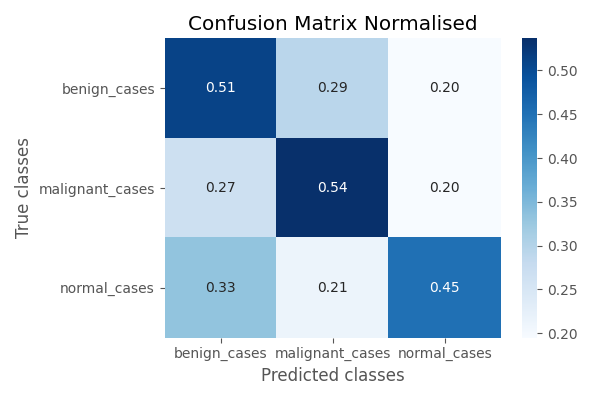
\includegraphics[width=0.8\textwidth]{figures/evaluation/common/CM-norm_basic-model_mini-MIAS-dataset.png}}
% \caption{\label{fig:evaluation-common-CM-norm_basic-model_mini-MIAS-dataset}Normalised confusion matrix of the classification results after training on the mini-MIAS dataset.}
% \end{figure}

% \subsection{Binary Classification}

% On the CBIS-DDSM dataset (binary classification problem), an accuracy of 65.36\% was initially achieved. Separating the types of mammograms between calcifications and masses revealed that higher accuracies could be achieved. Indeed, an accuracy of 70.36\% was reached when using only mammograms with masses, and 68.2\%  using only mammograms with calcifications (see Figure~\ref{fig:evaluation-cbisddsm-common-mass-vs-calc}).

% \begin{figure}[h]
% \centering
% \begin{subfigure}{.5\textwidth}
%   \centering
%   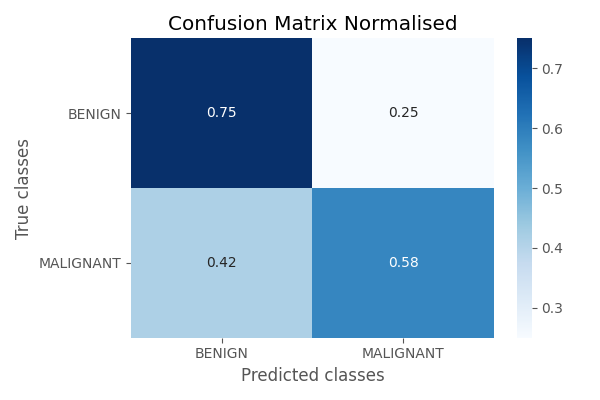
\includegraphics[width=\textwidth]{figures/evaluation/common/CM-norm_basic-model_CBIS-DDSM-dataset-Calc.png}
%   \caption{Mammograms with calcifications (70.36\%).}
%   \label{fig:evaluation-cbisddsm-common-calc}
% \end{subfigure}%
% \begin{subfigure}{.5\textwidth}
%   \centering
%   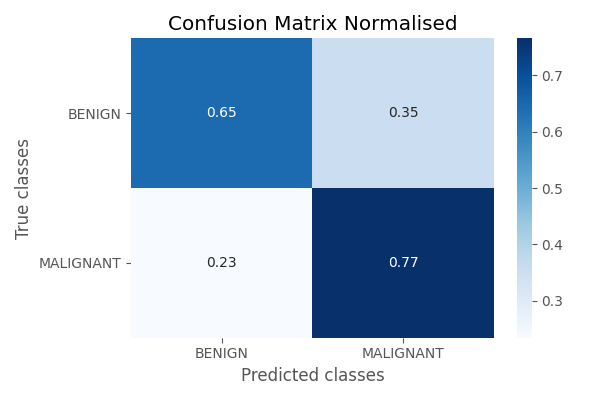
\includegraphics[width=\textwidth]{figures/evaluation/common/CM-norm_basic-model_CBIS-DDSM-dataset-Mass.png}
%   \caption{Mammograms with masses (68.2\%).}
%   \label{fig:evaluation-cbisddsm-common-mass}
% \end{subfigure}
% \caption{\label{fig:evaluation-cbisddsm-common-mass-vs-calc}Normalised confusion matrices between mammograms with calcifications and masses on the CBIS-DDSM dataset.}
% \end{figure}

% Minor optimisation attempts such as adding additional convolutional layers between the pre-trained VGG19 model and the fully connected layers lowered the accuracy to 55.07\%. Adding more convolutional and spooling layers before the VGG19 pre-trained model slightly increased the accuracy from 65.03\% to 65.36\%, but was much slower to train due to the increased number of trainable parameters that originated from the additional layers.

This section covers the bag-of-tricks approach mentioned in Section~\ref{sec:design-fine-tuning-bagoftricks}, where multiple deep learning techniques covered throughout Chapters~\ref{ch:chapter-litsurvey} \& \ref{ch:chapter-design} are experimented with to determine which improve the performance of the model.

%%%%%%%%%%%%%%%%%%%%%%%%%%%%%%%%%%%%%%%%%%%%%

\section{Model Used}

The model described in Section~\ref{sec:design-cnn-model-decision} is used across all the experiments below, using both VGG19 and MobileNetV2 as the base model (except for Section~\ref{sec:evaluation-cnn-model-experiment}), a fully connected MLP with 512, 32, 2 neurons, a dropout layer using $p=0.2$, the Adam optimiser and resized whole images. Only the dataset, batch size, input size, learning rate (0.001 or 0.0001), class weights, weight initialisation and type of mammograms vary across the experiments.

%%%%%%%%%%%%%%%%%%%%%%%%%%%%%%%%%%%%%%%%%%%%%

\section{Base CNN Architectures}
\label{sec:evaluation-cnn-model-experiment}

Five different CNN model architectures (VGG19, ResNet50, InceptionV3, DenseNet121 and MobileNetV2) are tested out as the model's base (pre-trained on ImageNet) using the model described in Section~\ref{sec:design-cnn-model-decision}. For this test, the CBIS-DDSM dataset is used with whole images resized to 512 x 512 pixels, a batch size of 2 and a learning rate of 0.0001.

\begin{table}[h]
\centering
\begin{tabular}{@{}lcccc@{}}
\toprule
\textbf{CNN Architecture} &
  \multicolumn{1}{l}{\textbf{Overall Accuracy}} &
  \multicolumn{1}{l}{\textbf{Precision}} &
  \multicolumn{1}{l}{\textbf{Recall}} &
  \multicolumn{1}{l}{\textbf{F1 Score}} \\ \midrule
\textit{\textbf{VGG19}}       & 63.96\%          & 63.73\%          & 63.96\%          & 63.83\%          \\
\textit{\textbf{ResNet50}}    & 61.00\%          & 64.23\%          & 61.00\%          & 61.23\%          \\
\textit{\textbf{InceptionV3}} & 62.71\%          & 62.52\%          & 62.71\%          & 62.60\%          \\
\textit{\textbf{DenseNet121}} & 64.74\%          & 65.81\%          & 64.74\%          & 65.03\%          \\
\textit{\textbf{MobileNetV2}} & \textbf{66.46\%} & \textbf{66.25\%} & \textbf{66.46\%} & \textbf{66.33\%} \\ \bottomrule
\end{tabular}
\caption{Results achieved on the test set when using different CNN architectures as the base model pre-trained on ImageNet weights.}
\label{tab:evaluation-cnn-models}
\end{table}

The results found in Table~\ref{tab:evaluation-cnn-models} clearly reveal that MobileNetV2 unlocks more performance than the others CNN architectures with a higher accuracy and F1 score. The original VGG19 architecture used during the development of the common pipeline is outperformed by more efficient models like DenseNet121 or MobileNetV2, but outperforms the ResNet50 and InceptionV3.\\

However, observing the training and testing runtimes in Figure~\ref{fig:evaluation-CNN_models_experiment-runtimes} reveals that VGG19 takes the longest time to train with 3h50m, whereas the more efficient MobileNetV2 architecture takes 2h46. Additionally, prediction runtime is 2.3 times faster with MobileNetV2 compared to VGG19, which is more useful for clinics as mammogram diagnosis results can be returned faster.

\begin{figure}[h]
\centerline{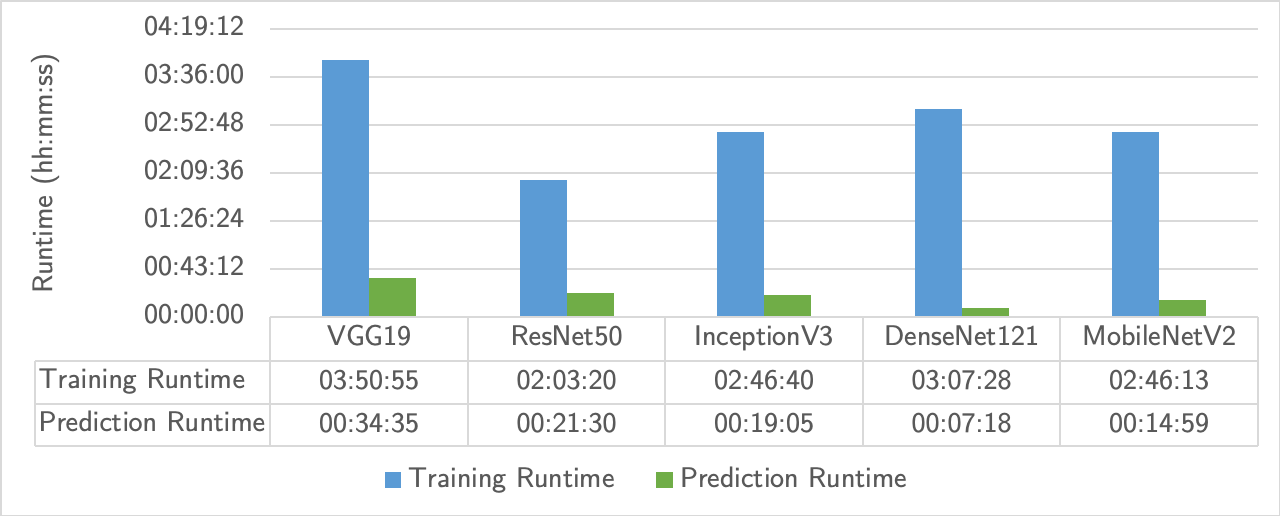
\includegraphics[width=\textwidth]{figures/evaluation/CNN_models_experiment/runtimes.png}}
\caption{\label{fig:evaluation-CNN_models_experiment-runtimes}Training and prediction runtimes when using different CNN architectures as the base model pre-trained on ImageNet.}
\end{figure}

%%%%%%%%%%%%%%%%%%%%%%%%%%%%%%%%%%%%%%%%%%%%%

\section{Class Weights}

Distinct variations of class weights are used on the CBIS-DDSM dataset to attempt to rectify the negative effects that can be introduced by imbalanced datasets without going through the process of data augmentation, which would considerably slow down the training time by a factor equal to the number of new images generated. Table~\ref{tab:evaluation-class-weights} reports the three class weight values that were tested using the imbalanced CBIS-DDSM dataset with whole images resized to 512 x 512 pixels, a batch size of 2 and a learning rate of 0.0001:
\begin{itemize}
    \item No class weights (dataset remains imbalanced);
    \item Balanced class weights:
    \begin{itemize}
        \item 0.907 for majority class (benign),
        \item 1.113 for minority class (malignant);
    \end{itemize}
    \item +50\% class weight for minority class:
    \begin{itemize}
        \item 1.0 for benign samples,
        \item 1.5 for malignant samples.
    \end{itemize}
\end{itemize}

\begin{table}[h]
\centering
\resizebox{\textwidth}{!}{%
\begin{tabular}{@{}llcccc@{}}
\toprule
\textbf{\begin{tabular}[c]{@{}l@{}}Base \\ model\end{tabular}} &
  \textbf{\begin{tabular}[c]{@{}l@{}}Class\\ weights\end{tabular}} &
  \multicolumn{1}{l}{\textbf{\begin{tabular}[c]{@{}l@{}}Overall \\ Accuracy\end{tabular}}} &
  \multicolumn{1}{l}{\textbf{Precision}} &
  \multicolumn{1}{l}{\textbf{Recall}} &
  \multicolumn{1}{l}{\textbf{F1 Score}} \\ \midrule
\multirow{3}{*}{\textit{\textbf{VGG19}}} &
  \textit{\textbf{None}} &
  62.25\% &
  63.66\% &
  62.25\% &
  62.58\% \\
 &
  \textit{\textbf{Balanced}} &
  63.96\% &
  63.94\% &
  63.96\% &
  63.95\% \\
 &
  \textit{\textbf{\begin{tabular}[c]{@{}l@{}}+50\%\\ minority\end{tabular}}} &
  61.15\% &
  62.16\% &
  61.15\% &
  61.45\% \\ \cmidrule(r){1-1}
\multirow{3}{*}{\textit{\textbf{MobileNetV2}}} &
  \textit{\textbf{None}} &
  65.83\% &
  66.33\% &
  65.83\% &
  66.01\% \\
 &
  \textit{\textbf{Balanced}} &
  \textbf{67.08\%} &
  \textbf{66.50\%} &
  \textbf{67.08\%} &
  \textbf{66.48\%} \\
 &
  \textit{\textbf{\begin{tabular}[c]{@{}l@{}}+50\%\\ minority\end{tabular}}} &
  65.05\% &
  65.19\% &
  65.05\% &
  65.12\% \\ \bottomrule
\end{tabular}%
}
\caption{Results achieved on the CBIS-DDSM test set when using different class weights (none, balanced and +50\% minority class) with VGG19 and MobileNet architectures as base model.}
\label{tab:evaluation-class-weights}
\end{table}

These results clearly depict how including balanced weights to the samples increases the accuracy across different base CNN models by 1.25-1.71\%. However, a manual weight increase for the minority class decreases the accuracy by 0.78-1.1\%, revealing the complexity of finding the right parameters for balancing datasets as the 50\% weight increase for malignant samples made the dataset even more unbalanced. The normalised confusion matrices found in Figures~\ref{fig:evaluation-class_weights_experiment-none} and \ref{fig:evaluation-class_weights_experiment-balanced} expose how including class weights leads to the model being more confused as many malignant samples are classified as benign.

\begin{figure}[h]
\centerline{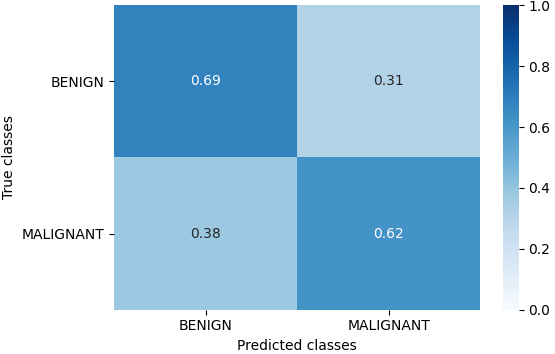
\includegraphics[width=0.75\textwidth]{figures/evaluation/class_weights_experiment/none.png}}
\caption{\label{fig:evaluation-class_weights_experiment-none}Normalised confusion matrix when no class weights are used with MobileNetV2 as the base model on the CBIS-DDSM dataset.}
\end{figure}

\begin{figure}[h]
\centerline{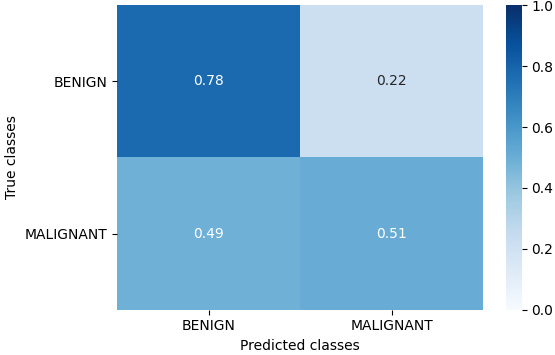
\includegraphics[width=0.75\textwidth]{figures/evaluation/class_weights_experiment/balanced.png}}
\caption{\label{fig:evaluation-class_weights_experiment-balanced}Normalised confusion matrix when balanced class weights are used with MobileNetV2 as the base model on the CBIS-DDSM dataset.}
\end{figure}

%%%%%%%%%%%%%%%%%%%%%%%%%%%%%%%%%%%%%%%%%%%%%

\section{Input Image Size}

Different image sizes are explored to determine their effect on the model's performance on the CBIS-DDSM dataset. For the smaller image sizes, larger batch sizes are used, whereas for the larger image sizes, smaller batch numbers are defined along with the extra convolutional and spooling layers mentioned in Section~\ref{sec:implementation-sequential-cnn-model} to make use of the larger image size as an attempt to learn lower-level features. The following image sizes are used:
\begin{itemize}
    \item 224 x 224 pixels (chosen as most CNNs pre-trained on ImageNet use this size) with batch size of 8;
    \item 512 x 512 pixels with batch size of 2;
    \item 1024 x 1024 pixels (with additional convolutional/spooling layers) with batch size of 2.
\end{itemize}

\begin{table}[h]
\centering
\resizebox{\textwidth}{!}{%
\begin{tabular}{@{}llccccc@{}}
\toprule
\textbf{\begin{tabular}[c]{@{}l@{}}Base\\ Model\end{tabular}} &
  \textbf{\begin{tabular}[c]{@{}l@{}}Whole \\ Image \\ Size \\ (pixels)\end{tabular}} &
  \multicolumn{1}{l}{\textbf{\begin{tabular}[c]{@{}l@{}}Extra \\ conv/\\ pool \\ layers\end{tabular}}} &
  \multicolumn{1}{l}{\textbf{\begin{tabular}[c]{@{}l@{}}Overall\\ Accuracy\end{tabular}}} &
  \multicolumn{1}{l}{\textbf{Precision}} &
  \multicolumn{1}{l}{\textbf{Recall}} &
  \multicolumn{1}{l}{\textbf{F1 Score}} \\ \midrule
\multirow{3}{*}{\textbf{VGG19}}       & \textit{\textbf{224 x 224}}   & No  & 63.96\%          & 65.33\%          & 63.96\%          & 64.28\%          \\
                                      & \textit{\textbf{512 x 512}}   & No  & 64.59\%          & 64.44\%          & 64.59\%          & 64.51\%          \\
                                      & \textit{\textbf{1024 x 1024}} & Yes & 59.28\%          & \textbf{66.94\%} & 59.28\%          & 58.43\%          \\ \cmidrule(r){1-1}
\multirow{3}{*}{\textbf{MobileNetV2}} & \textit{\textbf{224 x 224}}   & No  & 62.56\%          & 62.38\%          & 62.56\%          & 62.46\%          \\
                                      & \textit{\textbf{512 x 512}}   & No  & \textbf{67.08\%} & 66.50\%          & \textbf{67.08\%} & \textbf{66.48\%} \\
                                      & \textit{\textbf{1024 x 1024}} & Yes & OOM              & OOM              & OOM              & OOM              \\ \bottomrule
\end{tabular}%
}
\caption{Results achieved on the test set when using different input image sizes on the CBIS-DDSM dataset.}
\label{tab:evaluation-image-size}
\end{table}

The results in Table~\ref{tab:evaluation-image-size} clearly expose the accuracy increase by using 512 pixels-wide input size rather than 224, with a 0.63\% increase on VGG19 and 4.52\% increase on MobileNetV2. However, further increasing the input size to 1024 pixels has no positive effect as the accuracy drops by 4.52\% on VGG19 and leads to an Out Of Memory (OOM) error on MobileNetV2 despite lowering the batch size to 1.\\

\begin{figure}[H]
\centerline{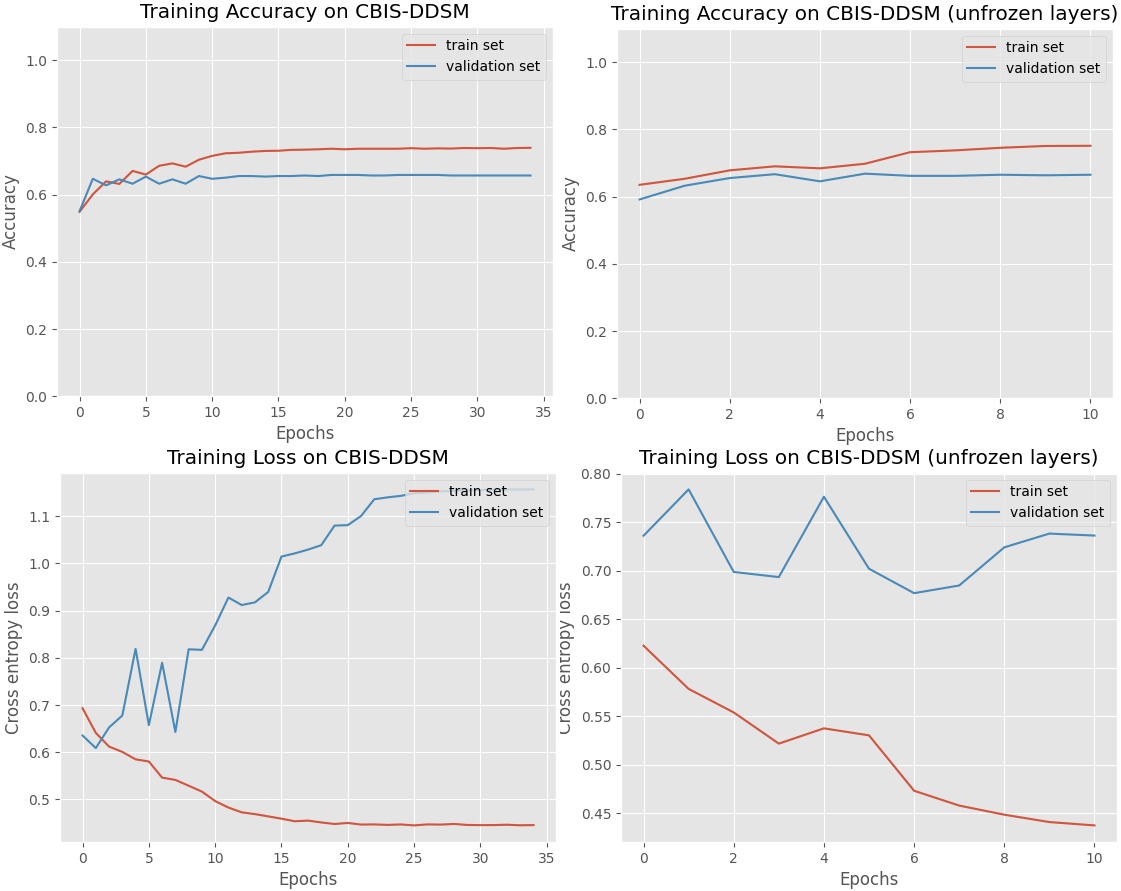
\includegraphics[width=1.2\textwidth]{figures/evaluation/image_size_experiment/training_summary.png}}
\caption{\label{fig:evaluation-image_size_experiment-training_summary}Evolution of the accuracy and loss during both training phases when testing 1024x1024 input size on VGG19.}
\end{figure}

Observing the evolution of the training accuracy and loss when using 1024 x 1024 pixels input size on VGG19 (see Figure~\ref{fig:evaluation-image_size_experiment-training_summary}), it can be seen that the validation loss increases while the training loss decreases and that both sets' training accuracies are increasing as well; which is a typical pattern of a model overfitting the data. Because the model is overfitting the data, a very high precision (66.94\%) but low recall (59.28\%) is witnessed in Table~\ref{tab:evaluation-image-size} for 1024x1024 input size, which is extremely bad as a BCD system that detects malignant cases as benign could lead to the death of the patient.\\

As expected, increasing the image size also increases the training runtime (see Figure~\ref{fig:evaluation-image_size_experiment-runtimes}), which is boosted by a factor of 2.4 when increasing from 224 to 512 pixels, and a factor of 2.8 from 512 to 1024 pixels on VGG19. However, another advantage of MobileNetV2 over VGG19 is that it scales better to larger input sizes as increasing the input from 224 to 512 pixels only raises the runtime by a factor of 1.54, and prediction times are quicker than VGG19 predictions (13.5 minutes on average for MobileNetV2 compared to 21.3 minutes for VGG19).

\begin{figure}[h]
\centerline{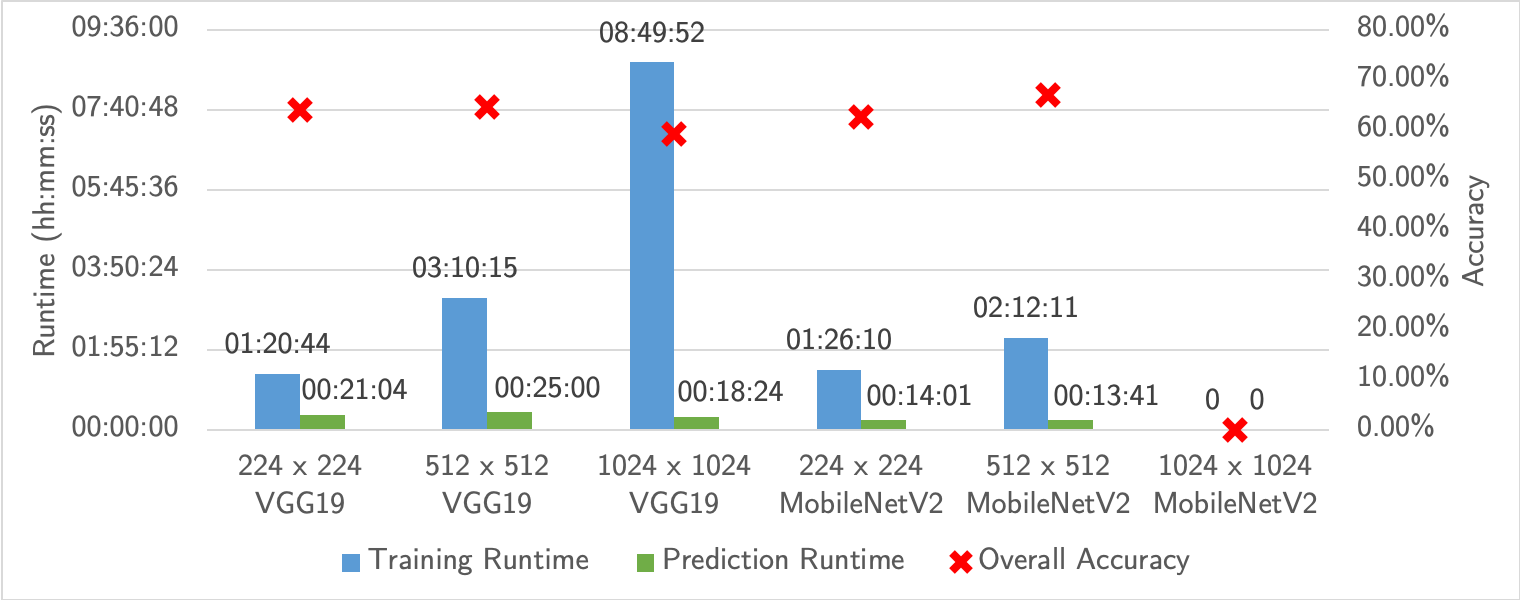
\includegraphics[width=\textwidth]{figures/evaluation/image_size_experiment/runtimes.png}}
\caption{\label{fig:evaluation-image_size_experiment-runtimes}Training and prediction runtimes when using different input image sizes.}
\end{figure}

Nevertheless, the accuracy/ training runtime trade-off is not primordial in breast cancer detection as the goal is to develop a system that can correctly diagnose early forms of cancers in mammograms as accurately as possible, regardless of the runtime. Ultimately, prediction runtimes will matter when used in clinics.

%%%%%%%%%%%%%%%%%%%%%%%%%%%%%%%%%%%%%%%%%%%%%

\section{Varying Amounts of Transfer Learning}
\label{sec:evaluation-transfer-learning}

This experiment consists of expanding upon the concept of transfer learning. Instead of using a CNN pre-trained on ImageNet, weights of a model trained on a \textit{binarised} mini-MIAS dataset are transferred to the CBIS-DDSM dataset. To binarise the mini-MIAS dataset, the normal cases are dropped altogether, resulting in a very small dataset of 115 abnormal images (64 benign and 51 malignant). The model is then trained on the binary mini-MIAS dataset and its final weights are saved. Four different experiments using an identical CNN architecture are tested to assess the effect of transfer learning from the binarised mini-MIAS dataset to the larger CBIS-DDSM dataset:
\begin{itemize}
    \item Transfer learning of all layer weights (Base CNN and fully connected layers instantiated with binary mini-MIAS weights);
    \item Transfer learning of fully connected layer weights (fully connected layers instantiated with binary mini-MIAS weights, base CNN layers instantiated with ImageNet weights);
    \item Transfer learning of ImageNet weights only (fully connected layers instantiated with random weights, base CNN layers instantiated with ImageNet weights);
    \item No transfer learning (Base CNN and fully connected layers instantiated with random weights).
\end{itemize}

\begin{table}[h]
\centering
\resizebox{\textwidth}{!}{%
\begin{tabular}{@{}lcccc@{}}
\toprule
\textbf{Transfer Learning} &
  \multicolumn{1}{l}{\textbf{Overall Accuracy}} &
  \multicolumn{1}{l}{\textbf{Precision}} &
  \multicolumn{1}{l}{\textbf{Recall}} &
  \multicolumn{1}{l}{\textbf{F1 Score}} \\ \midrule
\textit{\textbf{\begin{tabular}[c]{@{}l@{}}Full\\ mini-MIAS-binary\\ transfer learning\end{tabular}}}     & 63.18\% & 64.07\% & 63.18\% & 63.45\% \\ \cmidrule(r){1-1}
\textit{\textbf{\begin{tabular}[c]{@{}l@{}}MLP layers\\ mini-MIAS-binary \\ transfer learning\end{tabular}}} &
  \textbf{67.08\%} &
  \textbf{67.28\%} &
  \textbf{67.08\%} &
  \textbf{67.17\%} \\ \cmidrule(r){1-1}
\textit{\textbf{\begin{tabular}[c]{@{}l@{}}MobileNet layers\\ ImageNet\\ transfer learning\end{tabular}}} & 67.08\% & 66.50\% & 67.08\% & 66.48\% \\ \cmidrule(r){1-1}
\textit{\textbf{\begin{tabular}[c]{@{}l@{}}No transfer learning \\ (random weights)\end{tabular}}}        & 61.62\% & 61.00\% & 61.62\% & 61.17\% \\ \bottomrule
\end{tabular}%
}
\caption{Results achieved on the test set when using different amounts of transfer learning on the CBIS-DDSM dataset with the MobileNetV2 base model.}
\label{tab:evaluation-transfer-learning}
\end{table}

% \begin{table}[h]
% \centering
% \resizebox{\textwidth}{!}{%
% \begin{tabular}{@{}llcccc@{}}
% \toprule
% \textbf{\begin{tabular}[c]{@{}l@{}}Base\\ Model\end{tabular}} &
%   \textbf{\begin{tabular}[c]{@{}l@{}}Transfer\\ Learning\end{tabular}} &
%   \multicolumn{1}{l}{\textbf{\begin{tabular}[c]{@{}l@{}}Overall \\ Accuracy\end{tabular}}} &
%   \multicolumn{1}{l}{\textbf{Precision}} &
%   \multicolumn{1}{l}{\textbf{Recall}} &
%   \multicolumn{1}{l}{\textbf{F1 Score}} \\ \midrule
% \multirow{4}{*}{\textbf{VGG19 Common}} &
%   \textit{\textbf{\begin{tabular}[c]{@{}l@{}}Full \\ mini-MIAS-binary \\ transfer learning\end{tabular}}} &
%   57.87\% &
%   62.41\% &
%   57.88\% &
%   57.81\% \\ \cmidrule(lr){2-2}
%  &
%   \textit{\textbf{\begin{tabular}[c]{@{}l@{}}Fully \\ connected layers \\ mini-MIAS-binary \\ transfer learning\end{tabular}}} &
%   58.97\% &
%   60.43\% &
%   58.97\% &
%   59.33\% \\ \cmidrule(lr){2-2}
%  &
%   \textit{\textbf{\begin{tabular}[c]{@{}l@{}}ImageNet \\ transfer learning\end{tabular}}} &
%   59.44\% &
%   35.33\% &
%   59.44\% &
%   44.32\% \\ \cmidrule(lr){2-2}
%  &
%   \textit{\textbf{\begin{tabular}[c]{@{}l@{}}No transfer learning\\ (random weights)\end{tabular}}} &
%   60.37\% &
%   61.00\% &
%   60.37\% &
%   60.60\% \\ \cmidrule(r){1-2}
% \multirow{4}{*}{\textbf{MobileNetV2}} &
%   \textit{\textbf{\begin{tabular}[c]{@{}l@{}}Full \\ mini-MIAS-binary \\ transfer learning\end{tabular}}} &
%   63.18\% &
%   64.07\% &
%   63.18\% &
%   63.45\% \\ \cmidrule(lr){2-2}
%  &
%   \textit{\textbf{\begin{tabular}[c]{@{}l@{}}Fully \\ connected layers \\ mini-MIAS-binary \\ transfer learning\end{tabular}}} &
%   \textbf{67.08\%} &
%   \textbf{67.28\%} &
%   \textbf{67.08\%} &
%   \textbf{67.17\%} \\ \cmidrule(lr){2-2}
%  &
%   \textit{\textbf{\begin{tabular}[c]{@{}l@{}}ImageNet \\ transfer learning\end{tabular}}} &
%   \textbf{67.08\%} &
%   66.50\% &
%   \textbf{67.08\%} &
%   66.48\% \\ \cmidrule(lr){2-2}
%  &
%   \textit{\textbf{\begin{tabular}[c]{@{}l@{}}No transfer learning\\ (random weights)\end{tabular}}} &
%   61.62\% &
%   61.00\% &
%   61.62\% &
%   61.17\% \\ \cmidrule(r){1-2}
% \end{tabular}%
% }
% \caption{Results achieved on the test set when using different amounts of transfer learning on the CBIS-DDSM dataset using the custom MobileNetV2 and VGG19 models.}
% \label{tab:evaluation-transfer-learning}
% \end{table}

The results clearly indicate that the closer the weight initialisation were to the binary mini-MIAS dataset, the lower the test accuracy was, clearly indicating that the model did not generalise well to CBIS-DDSM mammograms. This could be linked to the advantages of random weight initialisations that give a better chance to the model to explore new combinations of weights rather than immediately converging towards a known solution. Indeed, Figure~\ref{fig:evaluation-individual-TL-training} shows how quickly the loss drops when using binary mini-MIAS weights, whereas the model slowly converges towards a lower loss when using random weight initialisations (no transfer learning).

\begin{figure}[h]
\centering
\begin{subfigure}{.5\textwidth}
  \centering
  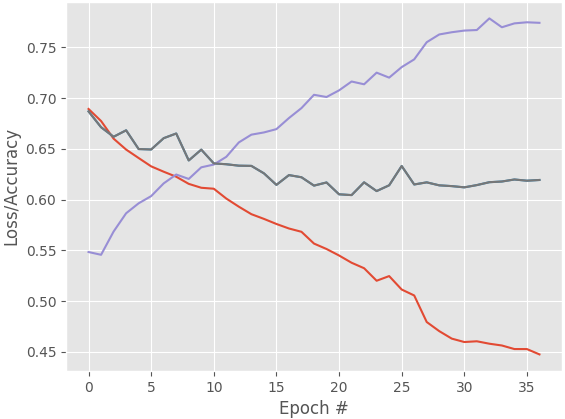
\includegraphics[width=\textwidth]{figures/evaluation/individual/TL-none.png}
  \caption{No transfer learning.}
  \label{fig:evaluation-individual-TL-none}
\end{subfigure}%
\begin{subfigure}{.5\textwidth}
  \centering
  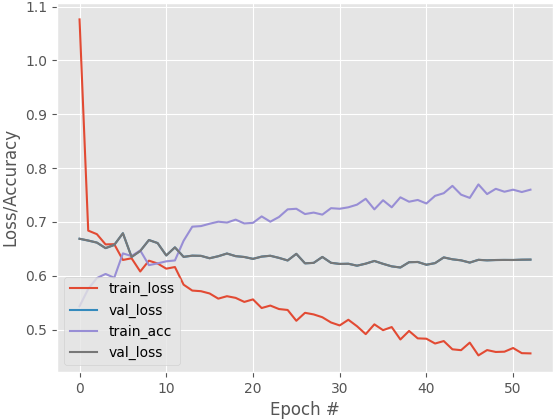
\includegraphics[width=\textwidth]{figures/evaluation/individual/TL-all.png}
  \caption{Binary mini-MIAS on all layers.}
  \label{fig:evaluation-individual-TL-all}
\end{subfigure}
\caption{\label{fig:evaluation-individual-TL-training}Evolution of the training accuracy and the training/validation losses across epochs with a learning rate of 0.001.}
\end{figure}

Additionally, it is worth noting that the training runtimes are similar across all tests, as it is the early stopping conditions (validation loss not decreasing) that dictates the stopping conditions.

% \section{Individual Optimisation Results}

% Using more advanced models than VGG19, which is a sequential CNN, such as InceptionV3, yielded poor results and required much longer training times. Indeed, the evolution of the validation loss visualised in Figure~\ref{fig:evaluation-individual-inceptionv3-poor-training}  confirms that  the InceptionV3 model highly overfits the data, suggested an urgent need for regularisation techniques such as Dropout.\\

% \begin{figure}[ht]
% \centerline{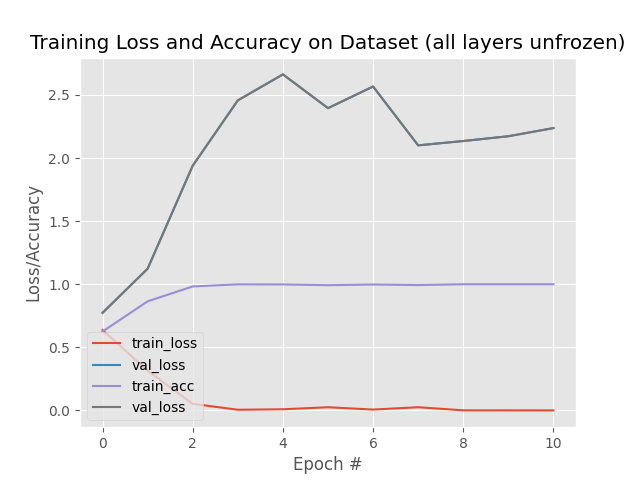
\includegraphics[width=0.8\textwidth]{figures/evaluation/individual/InceptionV3-poor-training.png}}
% \caption{\label{fig:evaluation-individual-inceptionv3-poor-training}Evolution of validation loss during training of the InceptionV3 model on the CBIS-DDSM dataset.}
% \end{figure}

% Potential future comparisons:
% \begin{itemize}
%     \item Different CNN models (VGG19, ResNet50V2, InceptionV3, Xception)
%     \item Using transfer learning (pre-trained model on ImageNet)
%     \item Using different types of mammograms (calcifications only, masses only, both)
% \end{itemize}

%%%%%%%%

\section{Mammogram Types}

To assess how the model would react to being fed only specific samples of a single mammogram type, the CBIS-DDSM dataset was separated into only masses samples and only calcifications samples. Three different experiments using identical an CNN architecture were tested:
\begin{itemize}
    \item All types of mammograms (masses + calcifications);
    \item Mass mammograms only;
    \item Calcification mammograms only.
\end{itemize}

\begin{table}[h]
\centering
\resizebox{\textwidth}{!}{%
\begin{tabular}{@{}llcccc@{}}
\toprule
\textbf{\begin{tabular}[c]{@{}l@{}}Base \\ Model\end{tabular}} &
  \textbf{\begin{tabular}[c]{@{}l@{}}Mammogram\\ type\end{tabular}} &
  \multicolumn{1}{l}{\textbf{\begin{tabular}[c]{@{}l@{}}Overall \\ Accuracy\end{tabular}}} &
  \multicolumn{1}{l}{\textbf{Precision}} &
  \multicolumn{1}{l}{\textbf{Recall}} &
  \multicolumn{1}{l}{\textbf{F1 Score}} \\ \midrule
\multirow{3}{*}{\textbf{VGG19}}       & \textit{\textbf{All}}            & 59.44\%          & 35.33\%          & 59.44\%          & 44.32\%          \\
                                      & \textit{\textbf{Masses}}         & 64.35\%          & 63.70\%          & 64.35\%          & 63.86\%          \\
                                      & \textit{\textbf{Calcifications}} & \textbf{66.67\%} & \textbf{67.05\%} & \textbf{66.67\%} & \textbf{66.80\%} \\ \midrule
\multirow{3}{*}{\textbf{MobileNetV2}} & \textit{\textbf{All}}            & \textbf{67.08\%} & \textbf{66.50\%} & \textbf{67.08\%} & \textbf{66.48\%} \\
                                      & \textit{\textbf{Masses}}         & 63.23\%          & 63.23\%          & 63.23\%          & 63.23\%          \\
                                      & \textit{\textbf{Calcifications}} & 63.12\%          & 64.57\%          & 63.12\%          & 63.39\%          \\ \bottomrule
\end{tabular}%
}
\caption{Results achieved on the test set when using different types of mammograms from the CBIS-DDSM dataset.}
\label{tab:evaluation-mammogram-types}
\end{table}

\begin{figure}[ht]
\centerline{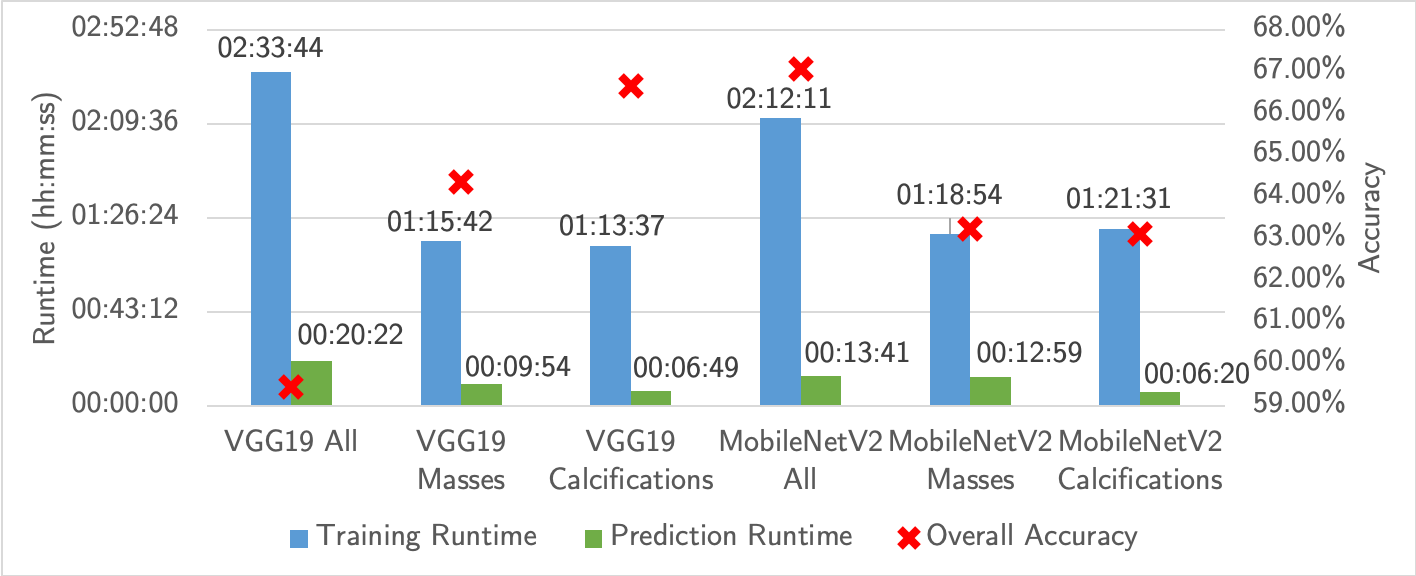
\includegraphics[width=\textwidth]{figures/evaluation/mammogram_type_experiment/runtimes.png}}
\caption{\label{fig:evaluation-mammogram_type_experiment-runtimes.png}Training and prediction runtimes when using different mammogram types.}
\end{figure}

These results show that the model learns the data much better when masses and calcifications are separated, reaching 64.35\% and 66.67\% accuracy respectively on the test set, but only managing 59.44\% when using the full CBIS-DDSM dataset. Indeed, the normalised confusion matrix indicates that all instances are classified as ``benign'' using the full dataset containing both types, which could indicate that the model gets confused when dealing with multiple views.\\

Harder to detect masses than calcifications \citep{Elter2009}.


\chapter{Conclusions}
\label{ch:chapter-conclusions}
To complete.

%%%%%%%%%%%%%%%%%%%%%%%%%%%%%%%%%%%%%%%%%%%%%%%%%%%%%%%%%%%%%%%%%%%%
%%%%%%%%%%%%%%%%%%%%%%%%%%%%%%%%%%%%%%%%%%%%%%%%%%%%%%%%%%%%%%%%%%%%
%%%%%%%%%%%%%%%%%%%%%%%%%%%%%%%%%%%%%%%%%%%%%%%%%%%%%%%%%%%%%%%%%%%%

\section{Achievements}

To complete.
    
%%%%%%%%%%%%%%%%%%%%%%%%%%%%%%%%%%%%%%%%%%%%%%%%%%%%%%%%%%%%%%%%%%%%
%%%%%%%%%%%%%%%%%%%%%%%%%%%%%%%%%%%%%%%%%%%%%%%%%%%%%%%%%%%%%%%%%%%%
%%%%%%%%%%%%%%%%%%%%%%%%%%%%%%%%%%%%%%%%%%%%%%%%%%%%%%%%%%%%%%%%%%%%

\section{Future Work}

Artefact removal (e.g. tags on the mammogram images).\\

More advanced image processing, as it is often an area where a large performance gains can be found \citep{Litjens2017}, by using techniques such as global contrast normalisation (GCN), local contrast normalisation, and Otsu’s threshold segmentation.\\

A lot of overfitting, better model training.

%%%%%%%%%%%%%%%%%%%%%%%%%%%%%%%%%%%%%%%%%%%%%%%%%%%%%%%%%%%%%%%%%%%%
%%%%%%%%%%%%%%%%%%%%%%%%%%%%%%%%%%%%%%%%%%%%%%%%%%%%%%%%%%%%%%%%%%%%
%%%%%%%%%%%%%%%%%%%%%%%%%%%%%%%%%%%%%%%%%%%%%%%%%%%%%%%%%%%%%%%%%%%%

\section{Limitations}
\label{sec:conclusions-limitations}

Data bias (dataset mainly white, different manifestations of breast cancer amongst different people)?\\

GPU size limited to 6GB (can  train on larger image sizes with large GPUs) \citep{Shen2017}.\\

When given new instances from the test dataset, the model predicts class labels. However, these do not indicate the confidence of the prediction, as it can be anywhere between the limit of  the decision boundary to the extreme opposite. Therefore, from a clinical point of view, it is hard to make a decision based on the  predictions made by the system. Ideally, a confidence metric in the form of a probability or a percentage would be coupled with the predictions  to  motivate the next  step after the diagnosis. For example, if the confidence of  a malignant tumour is high,  then a breast conserving surgery or chemotherapy can be recommended, whereas if the confidence is low, then further tests such as biopsies  can be recommended. % https://www.cancerresearchuk.org/about-cancer/breast-cancer/treatment/surgery/remove-just-area-cancer
    
%%%%%%%%%%%%%%%%%%%%%%%%%%%%%%%%%%%%%%%%%%%%%%%%%%%%%%%%%%%%%%%%%%%%
%%%%%%%%%%%%%%%%%%%%%%%%%%%%%%%%%%%%%%%%%%%%%%%%%%%%%%%%%%%%%%%%%%%%
%%%%%%%%%%%%%%%%%%%%%%%%%%%%%%%%%%%%%%%%%%%%%%%%%%%%%%%%%%%%%%%%%%%%

\section{Project Summary \& Reflections}

To complete.

The individual code developed for this dissertation can be found online at the following URL: \url{https://github.com/Adamouization/Breast-Cancer-Detection-and-Segmentation}. The code developed in common as a group at the beginning of the dissertation can be found online at the following URL: \url{https://github.com/Adamouization/Breast-Cancer-Detection-Code}.

\bibliography{Bibliography}

% \let\cleardoublepage\clearpage % don't automatically start appendix chapters on odd pages
\appendix

\chapter{Ethical Application Approval Letter}
\label{ch:appendix-ethical-approval-letter}
%%TC:ignore
Approval letter received on 18/06/2020 from the University of St Andrew's Teaching and Research Ethics Committee concerning the ethical application submitted on 03/06/2020 for this research project.

\clearpage

\includepdf[
    pages=1, 
    scale=0.85, 
    pagecommand=\label{sec:appendix-ethical-approval-letter-pdf}
]{figures/appendix/Approval Letter.pdf}
%%TC:endignore

\chapter{Languages \& Frameworks Comparison}
\section{Programming Languages}
\label{sec:appendix-programming-languages-comparison}

\begin{table}[h]
\centering
\resizebox{\textwidth}{!}{%
\begin{tabular}{l|l|l|l|l|}
\cline{2-5}
\multicolumn{1}{c|}{} &
  \multicolumn{1}{c|}{\textbf{Python}} &
  \multicolumn{1}{c|}{\textbf{Java}} &
  \multicolumn{1}{c|}{\textbf{R}} &
  \multicolumn{1}{c|}{\textbf{Javascript}} \\ \hline
\multicolumn{1}{|l|}{\textbf{Familiarity}} &
  Extremely familiar &
  Familiar &
  Unfamiliar &
  Familiar \\ \hline
\multicolumn{1}{|l|}{\textbf{\begin{tabular}[c]{@{}l@{}}Deep Learning \\ Libraries support\end{tabular}}} &
  \begin{tabular}[c]{@{}l@{}}Tensorflow, Keras, \\ PyTorch + ML suite \\ (NumPy, Pandas, \\ MatplotLib, Pandas)\end{tabular} &
  \begin{tabular}[c]{@{}l@{}}DL4J \\ \\ (Deeplearning4j)\end{tabular} &
  \begin{tabular}[c]{@{}l@{}}Tensorflow, \\ \\ Keras\end{tabular} &
  Tensorflow \\ \hline
\multicolumn{1}{|l|}{\textbf{\begin{tabular}[c]{@{}l@{}}Third-party\\ CUDA support\end{tabular}}} &
  Yes &
  Yes &
  Yes &
  Yes \\ \hline
\multicolumn{1}{|l|}{\textbf{\begin{tabular}[c]{@{}l@{}}Pre-trained\\ models support\end{tabular}}} &
  Yes &
  Yes &
  Yes &
  Yes \\ \hline
\multicolumn{1}{|l|}{\textbf{CNN support}} &
  Yes &
  Yes &
  Yes &
  Yes \\ \hline
\multicolumn{1}{|l|}{\textbf{Speed}} &
  Slow (interpreted) &
  Fast (compiled) &
  Fast (compiled) &
  Slow (interpreted) \\ \hline
\end{tabular}%
}
\caption{Table comparing the pros and cons of different programming languages when implementing a deep learning system.}
\label{tab:programming_languages_comparison}
\end{table}

\section{Deep Learning Frameworks}
\label{sec:appendix-keras_vs_pytorch}

Figures source: \url{https://keras.io/why_keras/}.

\begin{figure}[ht]
\centerline{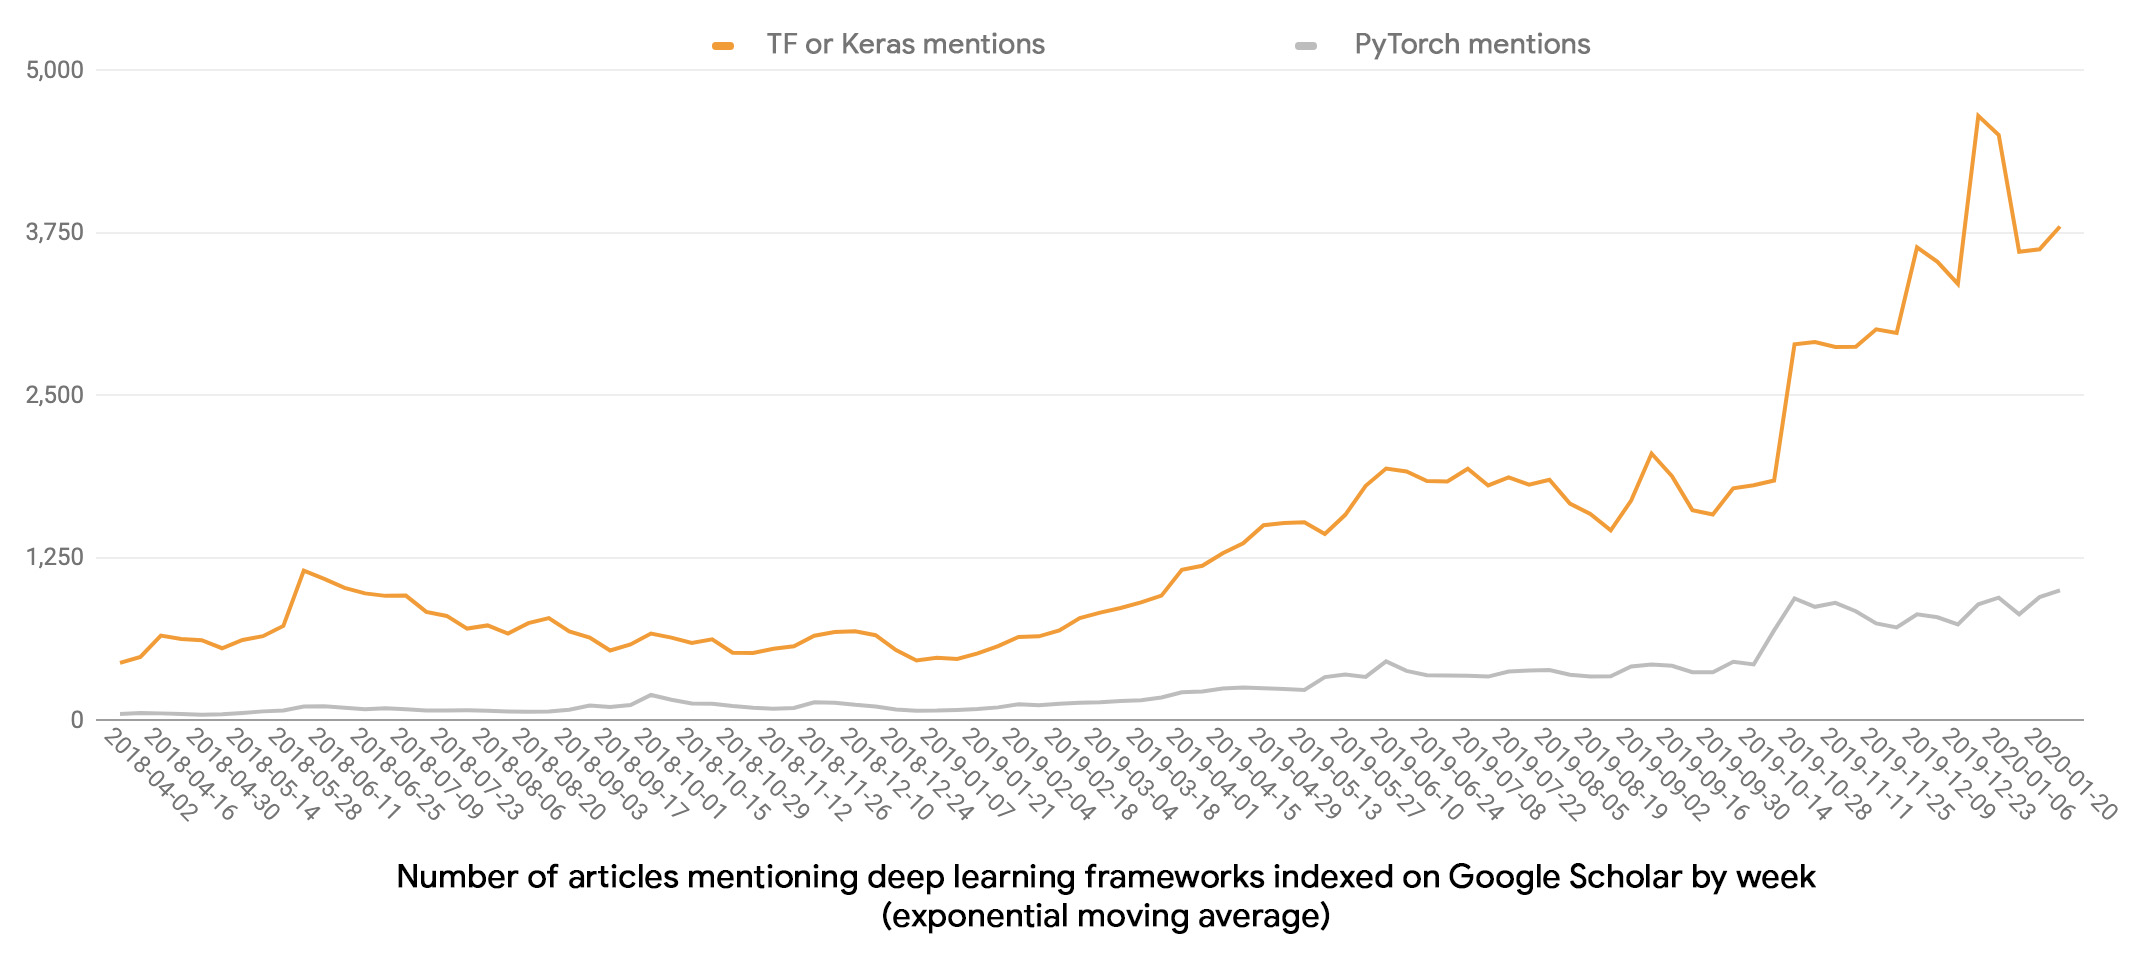
\includegraphics[width=1.1\textwidth]{figures/appendix/keras_vs_pytorch_mentions.jpeg}}
\caption{Chart highlighting the number of articles mentioning Keras and PyTorch. Figure downloaded from Keras website.}
\end{figure}

\begin{figure}[ht]
\centerline{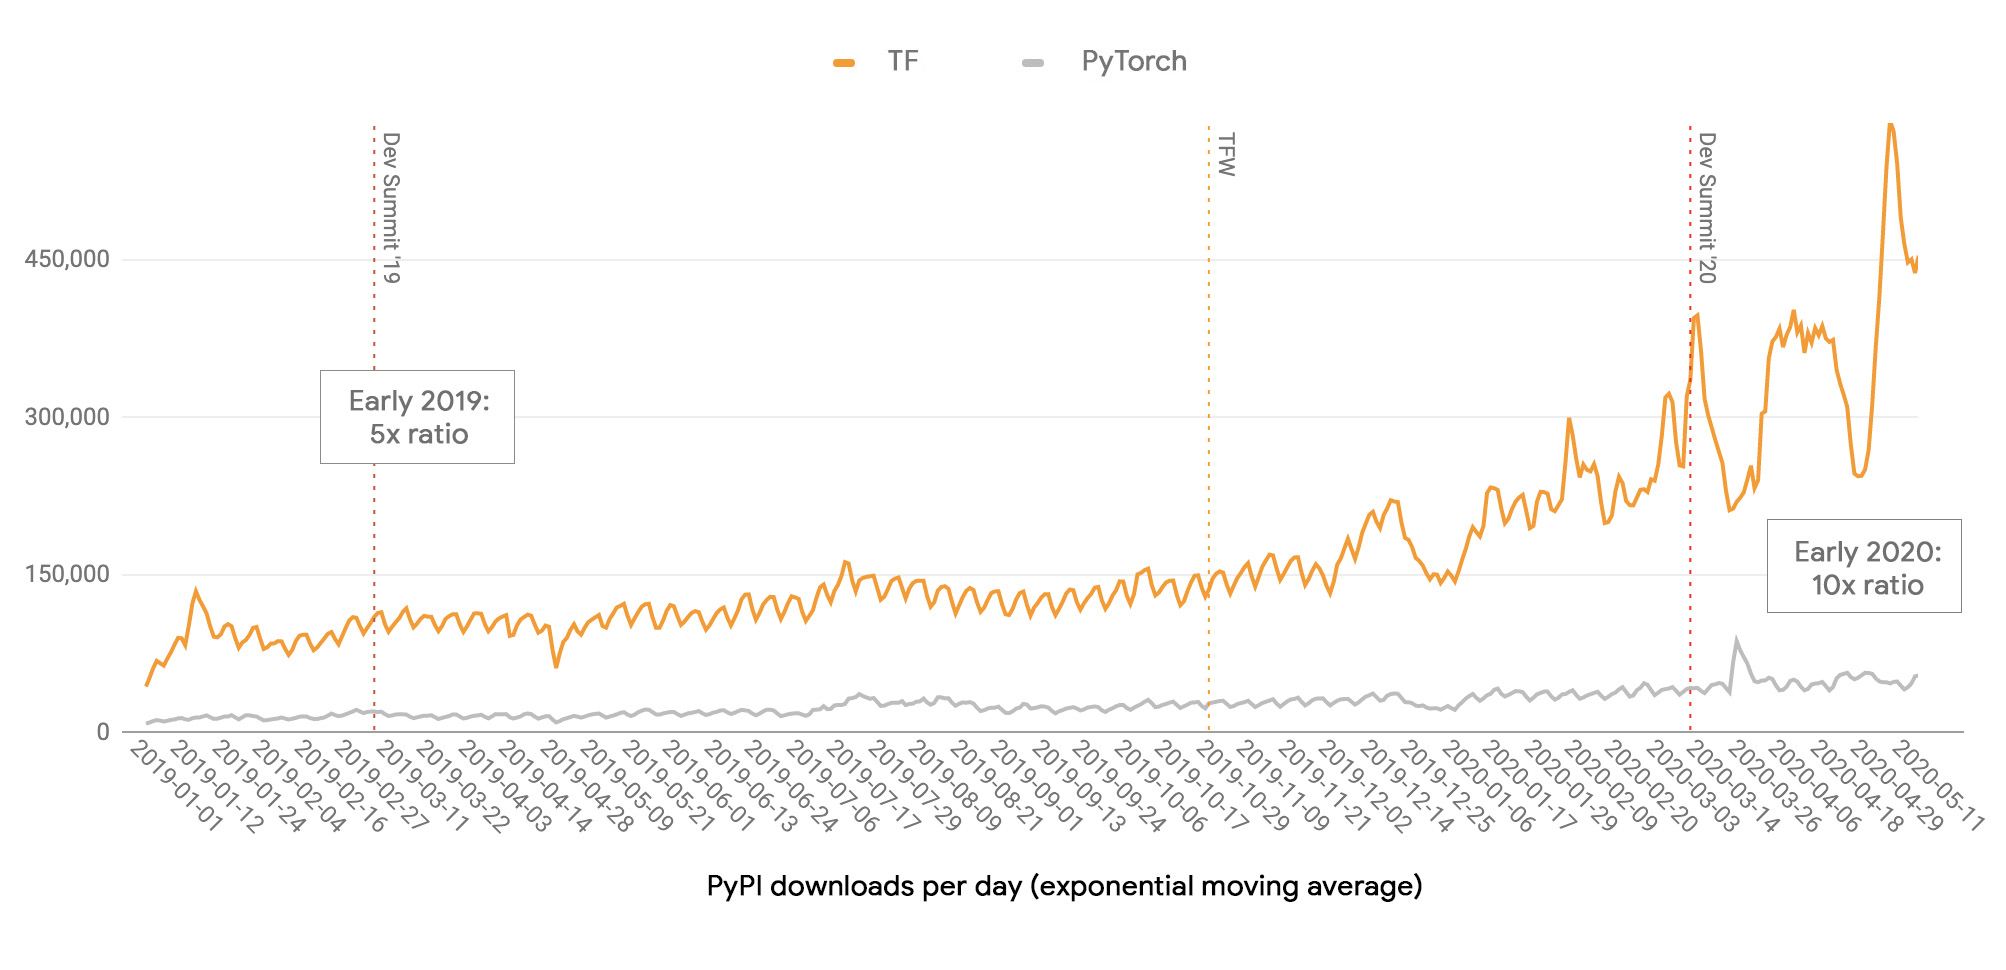
\includegraphics[width=1.1\textwidth]{figures/appendix/keras_vs_pytorch_downloads.jpg}}
\caption{Chart depicting the number of PyPI downloads for Keras and PyTorch. Figure downloaded from Keras website.}
\end{figure}

\chapter{Usage Instructions}
\label{ch:appendix-usage-instructions}
\section{Installation Instructions}

Start by cloning the GitHub repository (either the common or the individual code):

\begin{lstlisting}
cd ~/Projects
git clone https://github.com/Adamouization/Breast-Cancer-Detection-Code
\end{lstlisting}

Create a repository that will be used to install Tensorflow 2 with CUDA 10 for Python and activate the virtual environment for GPU usage:

\begin{lstlisting}
cd libraries/tf2
tar xvzf tensorflow2-cuda-10-1-e5bd53b3b5e6.tar.gz
sh build.sh
\end{lstlisting}

Activate the virtual environment:

\begin{lstlisting}
source /Breast-Cancer-Detection-Code/tf2/venv/bin/activate
\end{lstlisting}

`cd` into the `src` directory and run the code:

%%%%%%%%%%%%%%%%%%%%%%%%%%%%%%%%%%%%%%%%%%%%%%%%%%%%%%

\section{Individual Code Instructions}
\label{sec:appendix-individual-pipeline-instructions}

Run the code:

\begin{lstlisting}
main.py [-h] -d DATASET [-mt MAMMOGRAMTYPE] -m MODEL [-r RUNMODE] [-lr LEARNING_RATE] [-b BATCHSIZE] [-e1 MAX_EPOCH_FROZEN] [-e2 MAX_EPOCH_UNFROZEN] [-gs] [-roi] [-v]
\end{lstlisting}

where:
\begin{itemize}
    \item \textit{-h} is a  flag for help on how to run the code.
    \item \textit{DATASET} is the dataset to use. Must be either \textit{mini-MIAS}, \textit{mini-MIAS-binary} or \textit{CBIS-DDMS}.
    \item \textit{MAMMOGRAMTYPE} is the type of mammogram to use. Can be either \textit{calc}, \textit{mass} or \textit{all}.
    \item \textit{MODEL} is the model to use. Must be either \textit{VGG}, \textit{VGG-common}, \textit{Inception} or \textit{CNN}. Default value is \textit{VGG-common}.
    \item \textit{RUNMODE} is the learning rate used for the all the non-pre-trained ImageNet layers. Defaults to 1e-3. Must be a float.
    \item \textit{LEARNING\_RATE} is the batch size to use when training the model. Defaults to \textit{2}. Must be a positive integer.
    \item \textit{BATCHSIZE} is the batch size to use when training the model. Defaults to \textit{2}. Must be a positive integer.
    \item \textit{MAXEPOCHFROZEN} is the maximum number of epochs in the first training phrase (with frozen layers). Defaults to \textit{100}. Must be a positive integer.
    \item \textit{MAXEPOCHUNFROZEN} is the maximum number of epochs in the second training phrase (with unfrozen layers). Defaults to \textit{50}. Must be a positive integer.
    \item \textit{-gs} is a flag to run the grid search algorithm to determine the optimal hyperparameters for the CNN model. Defaults to \textit{False}.
    \item \textit{-roi} is a flag to use only cropped versions of the images around the ROI. Only usable with mini-MIAS dataset. Defaults to \textit{False}.
    \item \textit{-v} is a flag controlling verbose mode, which prints additional statements for debugging purposes. Defaults to \textit{False}.
\end{itemize}

Set the \textit{PYTHONHASHSEED} environment variable to 0 before the program starts for reproducible results (e.g. when using hash-based operations):

\begin{lstlisting}
PYTHONHASHSEED=0 main.py [...]
\end{lstlisting}

%%%%%%%%%%%%%%%%%%%%%%%%%%%%%%%%%%%%%%%%%%%%%%%%%%%%%%

\section{Common Pipeline Code Instructions}
\label{sec:appendix-common-pipeline-instructions}

Run the code:

\begin{lstlisting}
python main.py [-h] -d DATASET -m MODEL [-r RUNMODE] [-i IMAGESIZE] [-v]
\end{lstlisting}

where:
\begin{itemize}
    \item \textit{-h} is a  flag for help on how to run the code.
    \item \textit{DATASET} is the dataset to use. Must be either \textit{mini-MIAS} or \textit{CBIS-DDMS}.
    \item \textit{MODEL} is the model to use. Must be either \textit{basic} or \textit{advanced}.
    \item \textit{RUNMODE} is the mode to run in (\textit{train} or \textit{test}). Default value is \textit{train}.
    \item \textit{IMAGESIZE} is the image size to feed into the CNN model (\textit{small} - 512x512px; or \textit{large} - 2048x2048px). Default value is \textit{small}.
    \item \textit{-v} is a flag controlling verbose mode, which prints additional statements for debugging purposes.
\end{itemize}

%%%%%%%%%%%%%%%%%%%%%%%%%%%%%%%%%%%%%%%%%%%%%%%%%%%%%%

\section{Dataset Installation Instructions}

\subsection{mini-MIAS dataset}

This example will use the mini-MIAS dataset\footnote{mini-MIAS dataset: \url{http://peipa.essex.ac.uk/info/mias.html}}. After cloning the project, travel to the \textit{data/mini-MIAS} directory (there should be 3 files in it).\\

Create \textit{images\_original} and \textit{images\_processed} directories in this directory: 

\begin{lstlisting}
cd data/mini-MIAS/
mkdir images_original
mkdir images_processed
\end{lstlisting}

Move to the \textit{images\_original} directory and download the raw un-processed images:

\begin{lstlisting}
cd images_original
wget http://peipa.essex.ac.uk/pix/mias/all-mias.tar.gz
\end{lstlisting}

Unzip the dataset then delete all non-image files:

\begin{lstlisting}
tar xvzf all-mias.tar.gz
rm -rf *.txt 
rm -rf README 
\end{lstlisting}

Move back up one level and move to the \textit{images\_processed} directory. Create 3 new directories there (\textit{benign\_cases}, \textit{malignant\_cases} and \textit{normal\_cases}):

\begin{lstlisting}
cd ../images_processed
mkdir benign_cases
mkdir malignant_cases
mkdir normal_cases
\end{lstlisting}

Now run the python script for processing the dataset and render it usable with Tensorflow and Keras:

\begin{lstlisting}
python3 ../../../src/data_manipulations/mini-MIAS-initial-pre-processing.py
\end{lstlisting}

\subsection{CBIS-DDSM dataset}

These datasets are very large (exceeding 160GB) and more complex than the mini-MIAS dataset to use. They were downloaded by the University of St Andrews School of Computer Science computing officers onto \textit{BigTMP}, a 15TB filesystem that is mounted on the Centos 7 computer lab clients with NVIDIA GPUs, and that is usually used for storing large working data sets. Therefore, the download process of these datasets will not be covered in these instructions.\\

Our generated CSV files to use these datasets can be found in the \textit{/data/CBIS-DDSM} directory, but the mammograms will have to be downloaded separately directly from the source. The CBIS-DDSM dataset can be downloaded here: \url{https://wiki.cancerimagingarchive.net/display/Public/CBIS-DDSM#5e40bd1f79d64f04b40cac57ceca9272}.


\chapter{Remote Work Environment}
\label{ch:appendix-remote-work-environment}
Due to the corona virus pandemic that started on March 2020, and has been ongoing since the beginning of this research project (June 2020 to August 2020), work had to be conducted remotely.

\section{Coding environment}

Due to the physical lab machines equipped with the GPUs being inaccessible during the pandemic, these machines had to be remotely accessed through SSH. As it is not efficient to implement an entire deep learning pipeline through a command line interface, a \textit{Jupyter Lab} session is created on a lab computer port and forwarded back to a local personal computer.\\

This is done by first logging onto the lab machine via SSH, activating the virtual environment and launching the Jupyter Lab session (these instructions are added into a bash script to be quickly executed):

\begin{lstlisting}
ssh agj6@agj6.host.cs.st-andrews.ac.uk -t ssh agj6@pc5-026-l.cs.st-andrews.ac.uk
source /cs/scratch/agj6/tf2/venv/bin/activate
cd ~/Projects/Breast-Cancer-Detection-and-Segmentation
jupyter lab --no-browser --port=8888
\end{lstlisting}

Keeping the first SSH session alive, a second terminal session is opened, and the port forwarding from the lab machine  to the personal computer is carried out using  the following command:

\begin{lstlisting}
nohup ssh -J agj6@agj6.host.cs.st-andrews.ac.uk agj6@pc5-026-l.cs.st-andrews.ac.uk -L 8888:localhost:8888 -N
\end{lstlisting}

To prevent the two SSH sessions from being automatically killed, some SSH settings are added to the ``\textit{/etc/ssh/ssh\_config}'' file, making the personal computer send a null packet to the lab machine every 5 minutes:

\begin{lstlisting}
Host *
    ServerAliveInterval 300
    ServerAliveCountMax 2
\end{lstlisting}

Finally, \url{http://localhost:8888}  is visited on a web browser to gain access to  the Jupyter Lab interface, containing a menu bar, a file explorer, code editor and command line for running python files (see Figure~\ref{fig:appendix-jupyter_interface}).

\begin{figure}[ht]
\centerline{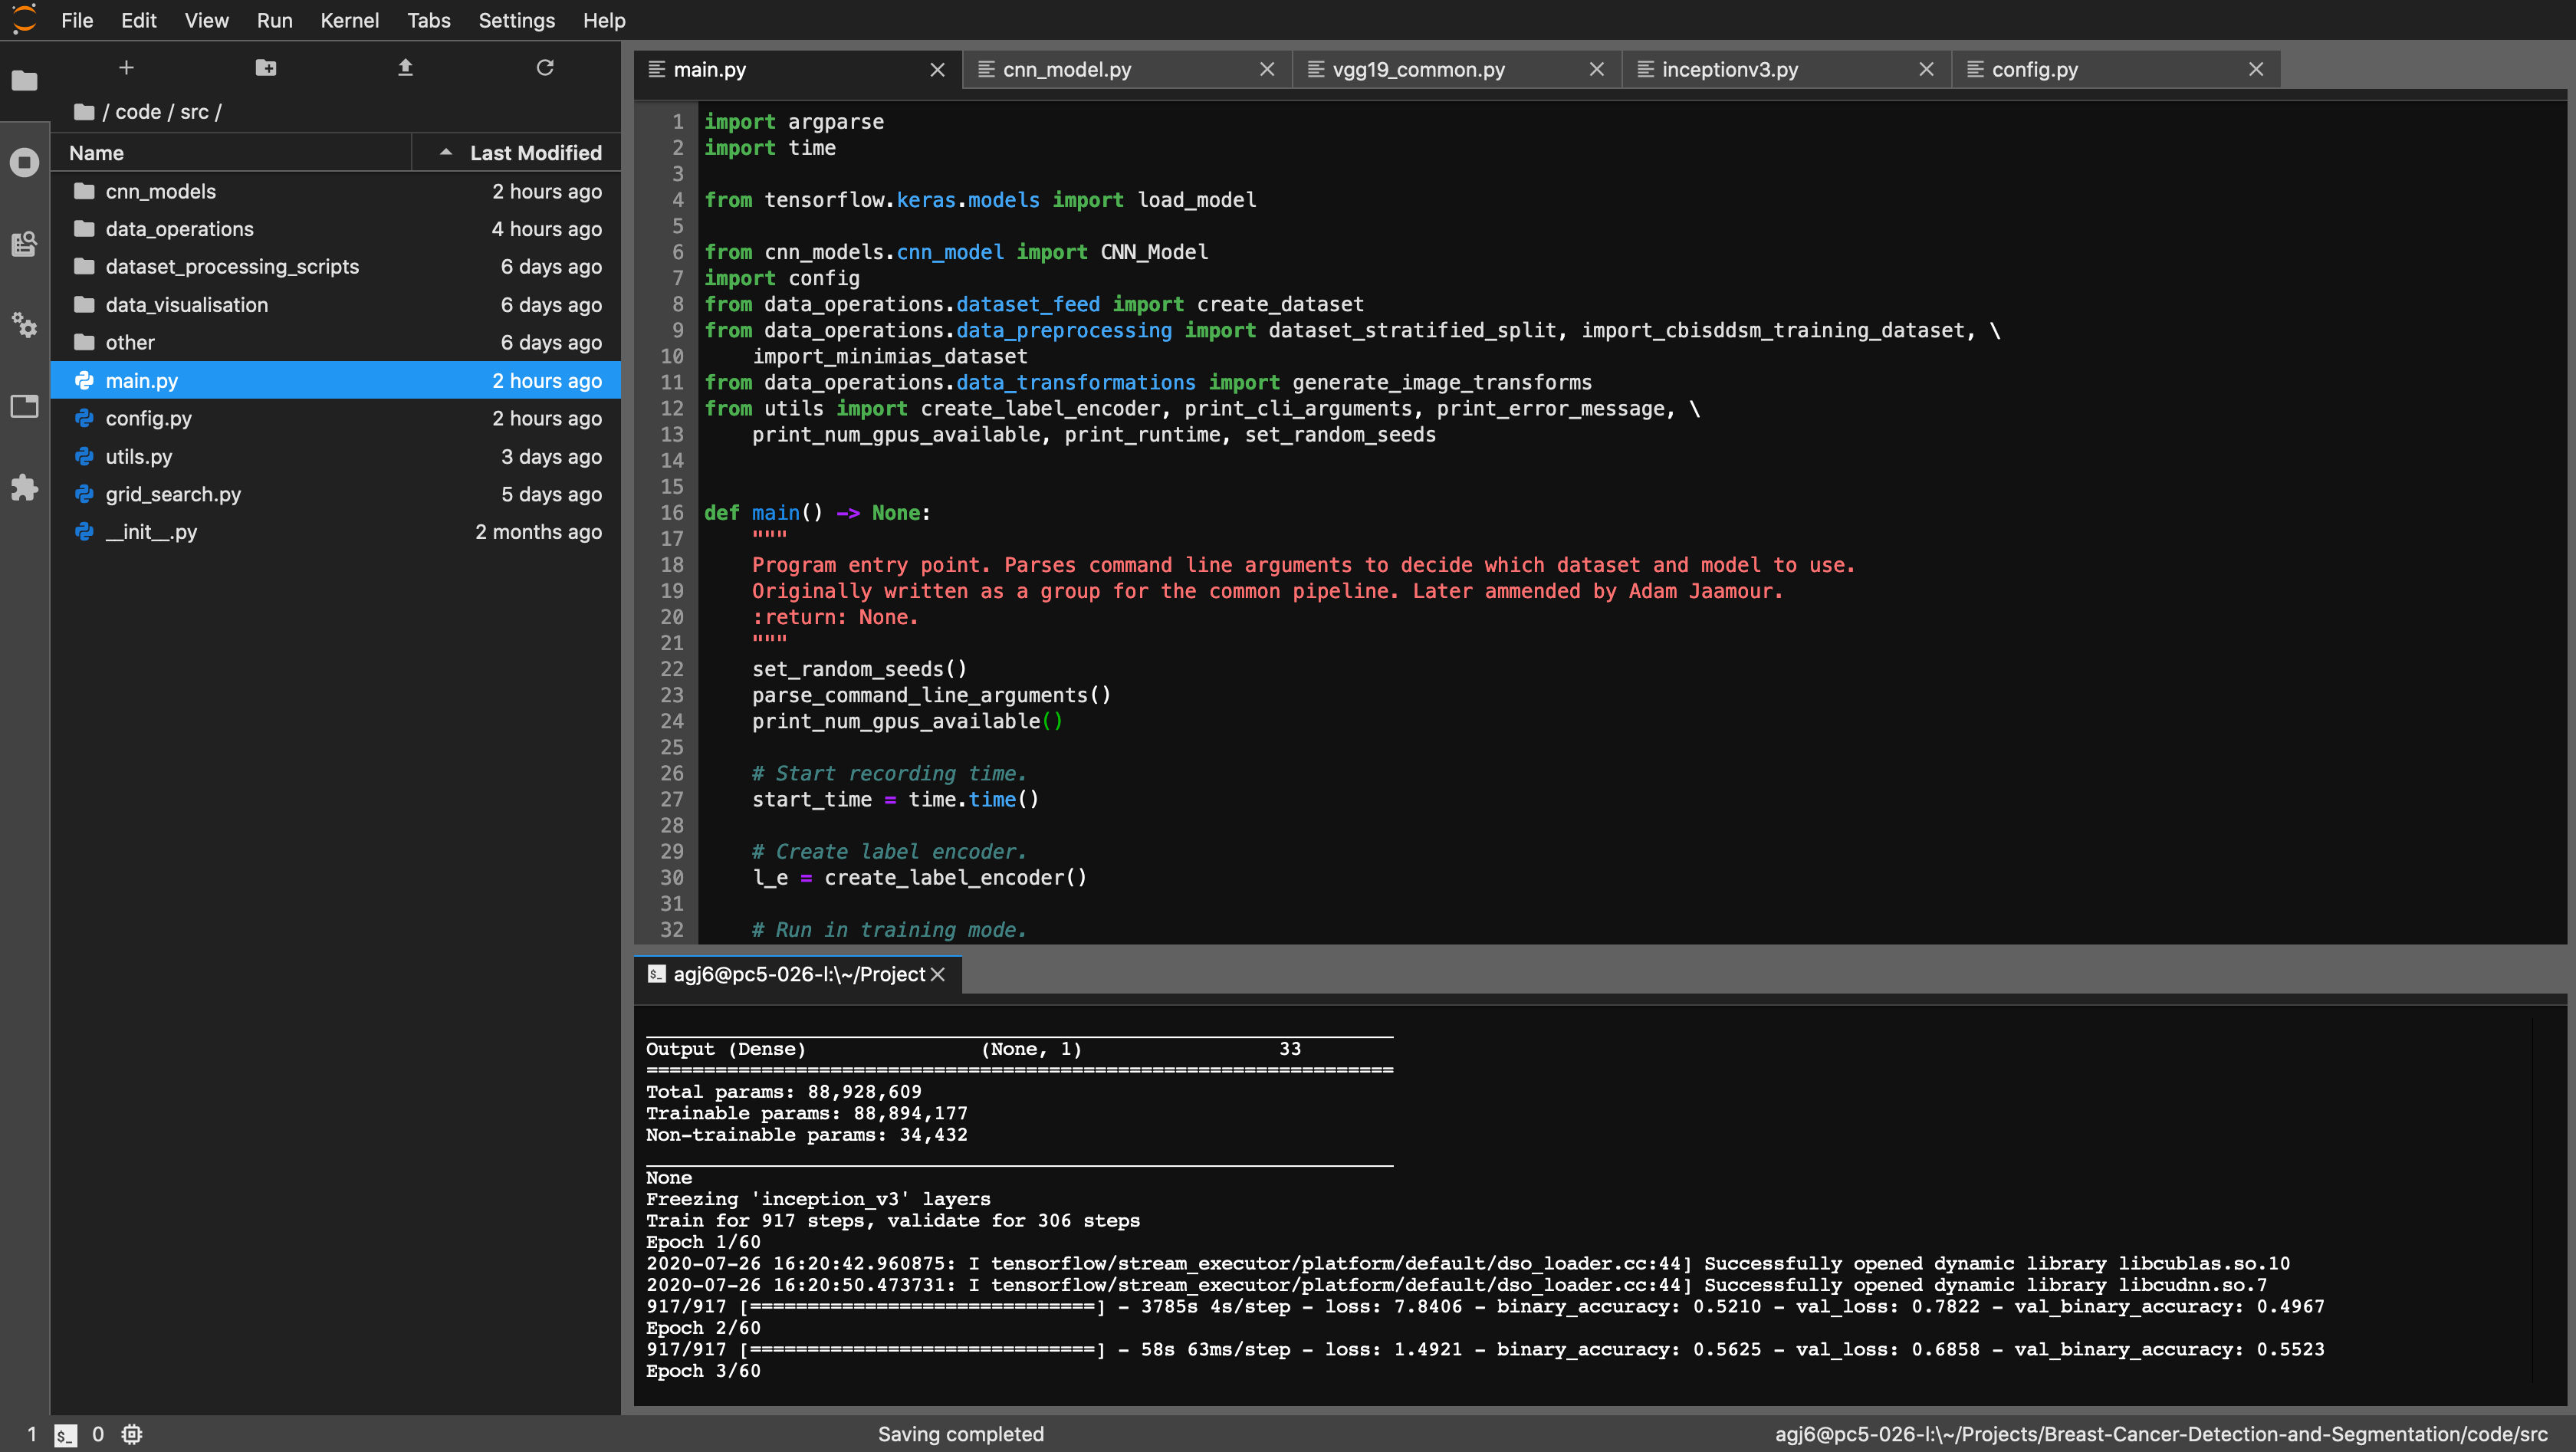
\includegraphics[width=\textwidth]{figures/appendix/jupyter_interface.png}}
\caption{\label{fig:appendix-jupyter_interface}Screenshot of the Jupyter Lab interface used to implement the project.}
\end{figure}

\section{Code collaboration}

For the group work part of the project, the code was collaboratively written and version controlled using GitHub, making use of the pull requests and merging features to combine code written by each group member. The code developed as a group can be found online at the following URL: \url{https://github.com/Adamouization/Breast-Cancer-Detection-Code}.

\section{Supervisor meetings}

Weekly video meetings with the project supervisor, Dr David Harris-Birtill, and the project co-supervisor, Lewis McMillan, were planned once per week via Microsoft Teams. Additional meetings with the other group members, Ashay Patel and Shuen-Jen Chen, were conducted via Microsoft Teams as well.

\chapter{Team Meeting Summaries}
\label{ch:appendix-team-meeting-summaries}
This appendix contains the summary of the team meetings carried out during the development of the common deep learning pipeline from 24/06/2020 to 09/07/2020. They include the attendance, the matters discussed and the tasks set for the next meeting, 

\clearpage
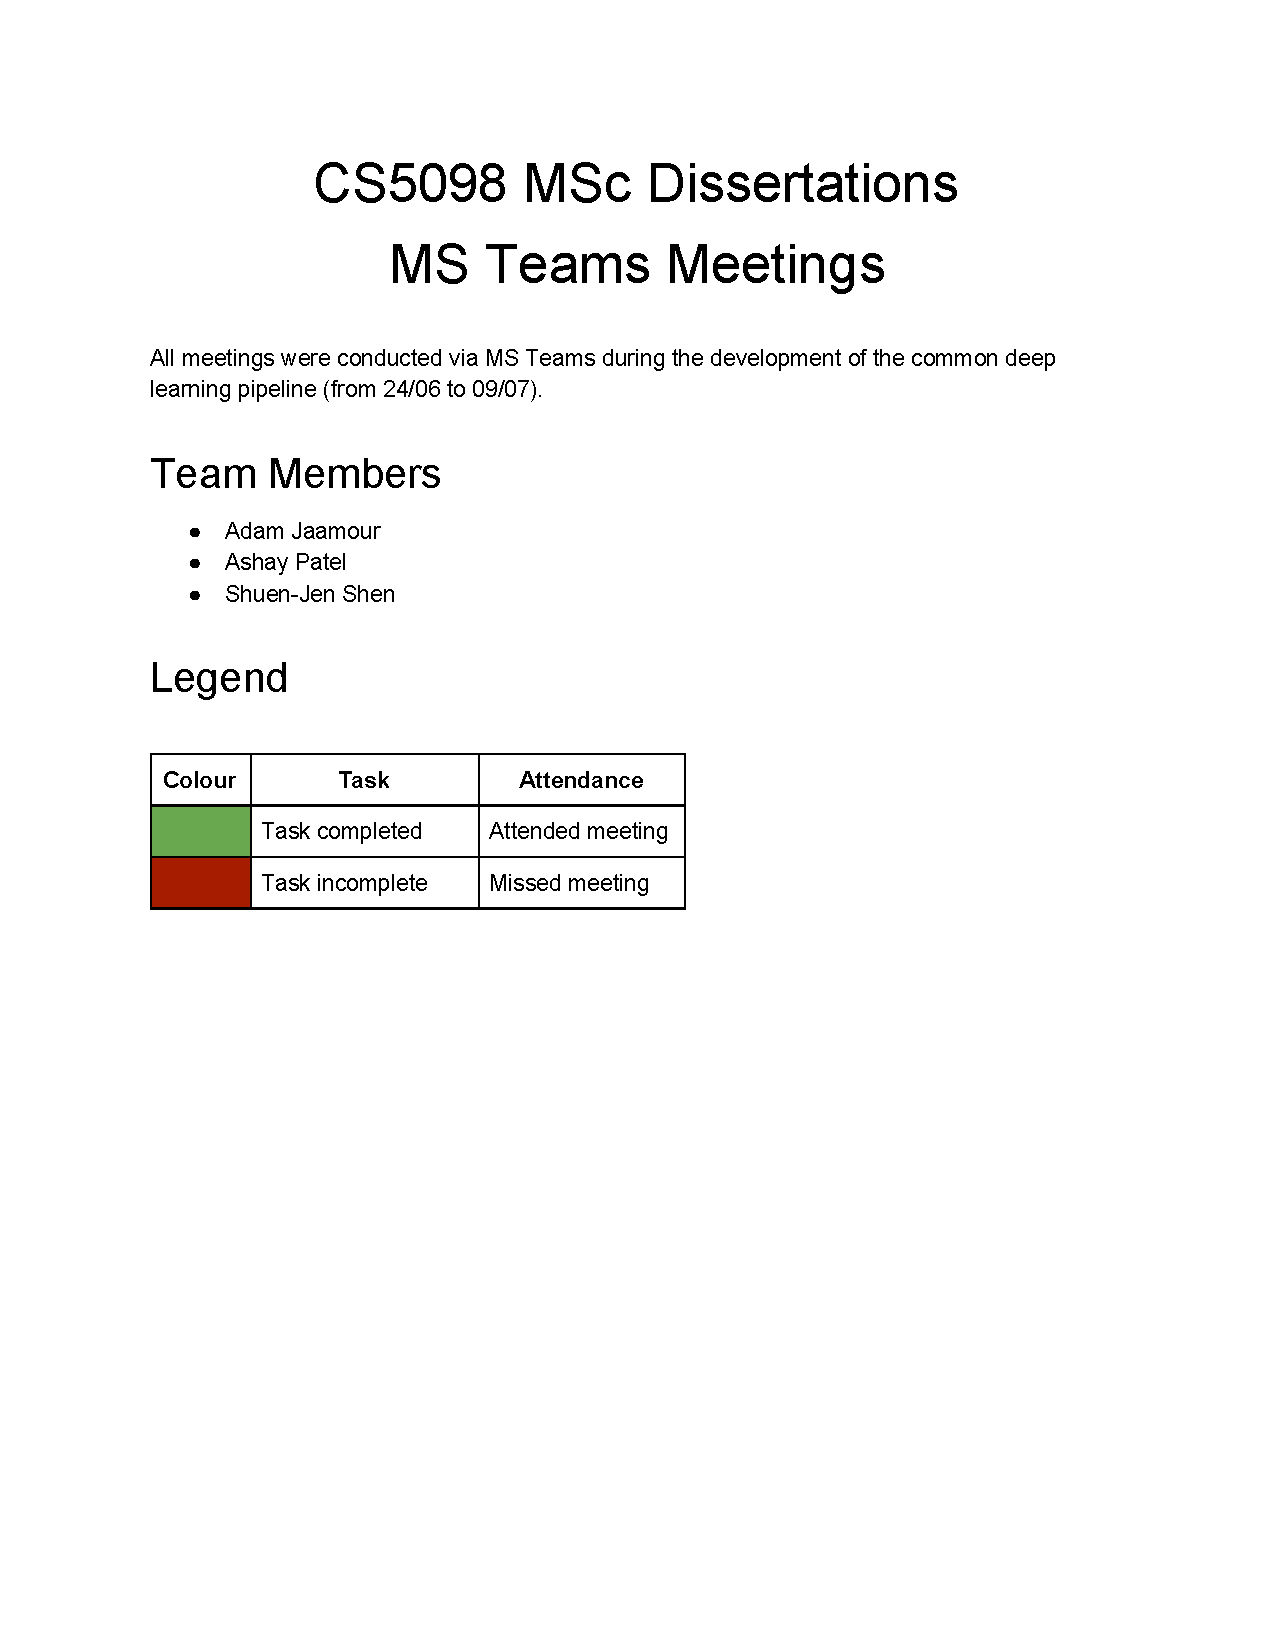
\includepdf[pages={1,2,3,4,5,6,7,8,9},pagecommand={},scale=0.88]{figures/appendix/team_meetings.pdf}

\chapter{Coding Project Structure}
\label{ch:appendix-coding-project-structure}
%%TC:ignore
Structure of the individual implementation  found in Figure~\ref{fig:appendix-project_structure}.

\begin{figure}[h]
\centerline{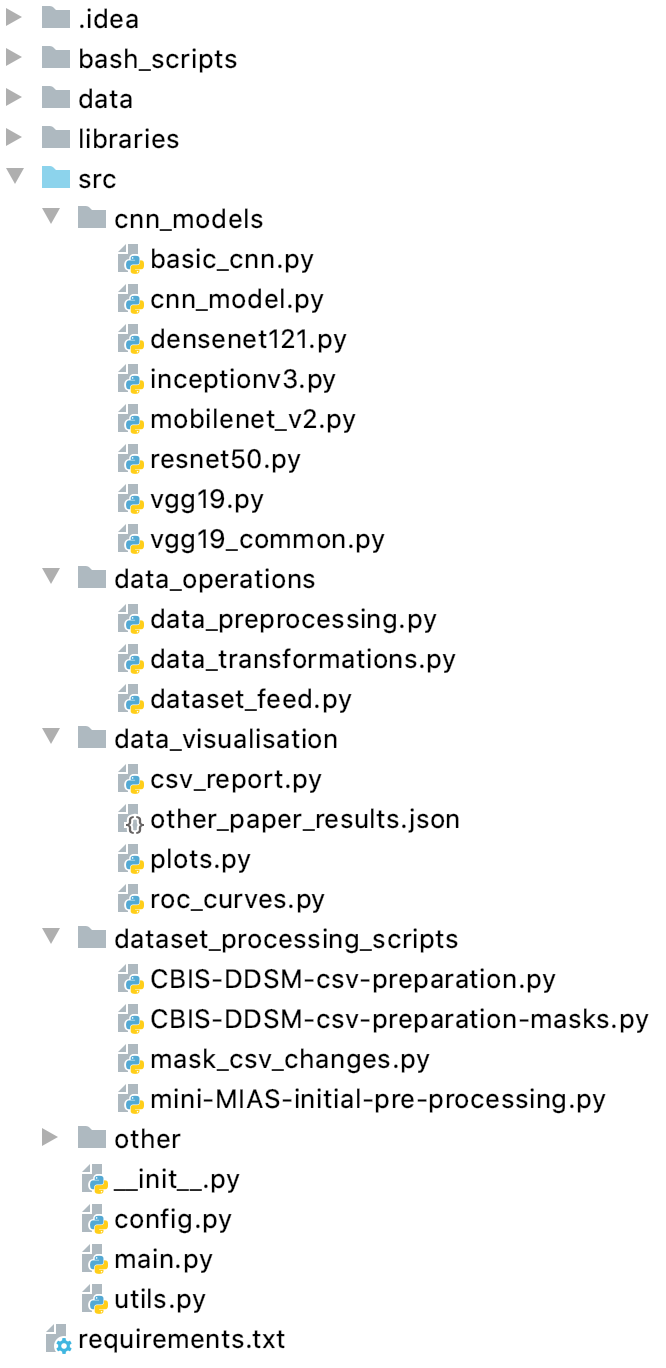
\includegraphics[width=0.70\textwidth]{figures/appendix/project_structure.png}}
\caption{\label{fig:appendix-project_structure}Screenshot of the project structure.}
\end{figure}
%%TC:endignore

\end{document}